\documentclass[10pt]{amsart}
\usepackage[a4paper,margin=23mm]{geometry}
\usepackage{amsmath,amssymb,amsthm,mathtools,hyperref,graphicx,xspace,letltxmacro,xpatch}
\usepackage[english]{babel}
\newtheorem{theo}{Theorem}[section]
\newtheorem{lemm}[theo]{Lemma}\newtheorem{prop}[theo]{Proposition}\newtheorem{coro}[theo]{Corollary}\newtheorem{conj}[theo]{Conjecture}
\theoremstyle{definition}\newtheorem{defi}[theo]{Definition}\newtheorem{rema}[theo]{Remark}\newtheorem{exam}[theo]{Example}\newtheorem{exem}[theo]{Example}\newtheorem{nota}[theo]{Notation}
\newcommand{\ie}{i.e.}\newcommand{\eg}{e.g.}\newcommand{\resp}{resp.}\newcommand{\skpt}{\par\smallskip\noindent}
\emergencystretch=3em\pagestyle{plain}
%~Mouliné par MaN_auto v.0.27.3 2023-07-31 10:11:49

\usepackage{mathrsfs}



\makeatletter
\def\editors#1{%
\def\editor@name{#1}
\if@francais
\def\editor@string{Recommand\'e par les \'editeurs \editor@name.}
\else
\def\editor@string{Recommended by Editors \editor@name.}
\fi}   
\makeatother
\newcommand{\noopsort}[1]{}






%\AtBeginDocument{
%\newtheorem{myname}[cdrthm]{My beautiful theorem} }


\newcommand*\p{\partial}
\newcommand*\R{\mathbb R}
\newcommand*\N{\mathbb N}
\newcommand*\C{\mathbb C}
\newcommand{\bbM}{\mathbb{M}}

\newcommand*\ddef{\stackrel{\rm def}{=}}
\renewcommand{\sc}{\mathrm{sc}}
\newcommand{\amm}{\mathrm{am}}
\newcommand{\EK}{\mathrm{EK}}
\newcommand{\FP}{\mathrm{FP}}
\newcommand{\phl}{\mathrm{ph}}
\newcommand{\Err}{\mathrm{Err}}
\newcommand{\Imm}{\mathrm{Im}}
\newcommand{\Rel}{\mathrm{Re}}
\newcommand{\locc}{\mathrm{loc}}
\newcommand{\divv}{\mathrm{div}}
\newcommand{\Span}{\mathrm{Span}}

\newcommand*\BE{\mathcal{E}}
\newcommand*\BO{\mathcal{O}}
\newcommand*\BC{\mathcal{C}}
\newcommand*\BA{\mathcal{A}}
\newcommand*\BH{\mathcal{H}}
\newcommand*\BI{\mathcal{I}}
\newcommand*\BN{\mathcal{N}}
\newcommand*\BK{\mathcal{K}}
\newcommand*\BS{\mathcal{S}}
\newcommand*\BT{\mathcal{T}}
\newcommand*\BW{\mathcal{W}}
\newcommand*\BX{\mathcal{X}}
\newcommand*\BY{\mathcal{Y}}

\newcommand{\bfun}{\mathbf{1}}

\newcommand*\be{\begin{equation}}
\newcommand*\ee{\end{equation}}
\newcommand*\ds{\displaystyle}
\newcommand*\ex{{\sf e}}

\newcommand*\Fou{\mathscr{F}}
\newcommand*\Sch{\mathscr{S}}

\newcommand*\cs{{\mathfrak c}}
\renewcommand*\u{\mathfrak{u}}
\newcommand{\fkL}{\mathfrak{L}}

\newcommand*\ii{\infty}
\newcommand*\gs{\geqslant }
\newcommand*\ls{\leqslant }
\newcommand*\e{\varepsilon}
\newcommand*\ep{\epsilon}
\newcommand*\lne{\lvert \ln \varepsilon \rvert}
\newcommand*\fin{\hfill $\lrcorner$}
\renewcommand*\t{\tilde}
\renewcommand*\a{\alpha}
\newcommand*\s{\sigma}
\newcommand*\G{\Gamma}
\newcommand*\vp{\varphi}

\newcounter{stepcount}
%\newenvironment{step}{\refstepcounter{stepcount}\begin{proof}[Step~\thestepcount]}{\let\qed\relax\end{proof}}


\newenvironment{step}[1]{\refstepcounter{stepcount}\begin{proof}[{Step~\thestepcount}{\;(#1)}]}{\let\qed\relax\end{proof}}
%%%%%%%%%%%%%%%%%%%%%%%%%%%%%%%%%%%%%%%%%%%%%%%%%%%%%%%%%%%%%%%%


\graphicspath{{./figures/}}

\newcommand*{\mk}{\mkern -1mu}
\newcommand*{\Mk}{\mkern -2mu}
\newcommand*{\mK}{\mkern 1mu}
\newcommand*{\MK}{\mkern 2mu}

%\hypersetup{urlcolor=purple, linkcolor=blue, citecolor=red}
\newcommand*{\relabel}{\renewcommand{\labelenumi}{(\theenumi)}}
\newcommand*{\romanenumi}{\renewcommand*{\theenumi}{\roman{enumi}}}
\newcommand*{\Romanenumi}{\renewcommand*{\theenumi}{\Roman{enumi}}}
\newcommand*{\alphenumi}{\renewcommand*{\theenumi}{\alph{enumi}}}
\newcommand*{\Alphenumi}{\renewcommand*{\theenumi}{\Alph{enumi}}}
\newcommand*{\romenumi}{\renewcommand*{\theenumi}{\roman{enumi}'}\relabel}

\let\oldtilde\tilde
\renewcommand*{\tilde}[1]{\mathchoice{\widetilde{#1}}{\widetilde{#1}}{\oldtilde{#1}}{\oldtilde{#1}}}
\let\oldhat\hat
\renewcommand*{\hat}[1]{\mathchoice{\widehat{#1}}{\widehat{#1}}{\oldhat{#1}}{\oldhat{#1}}}
\let\oldforall\forall
\renewcommand*{\forall}{\mathrel{\oldforall}}
%%%%%%%%%%%%%%%%%%%%%%%%%%%%%%%%%%%%%%%%%%%%%%%%%%%%%%%%%%

\title{Smooth transonic branch of rarefaction pulses for two-dimensional nonlinear Schrodinger equations}
\author{Chiron, David}
\date{doi:10.5802/ahl.178; CC BY 4.0}
\begin{document}
\maketitle
\noindent\textit{Editorial note.} Only selected author result counted; complete original mathematical body and bibliography retained. Native PDF vector Forms and original raster/soft mask retained; class frontmatter and web-only definitions omitted from rendering preamble.\par\medskip
\noindent\textit{Editorial note.} A native line break immediately after begin proof is preceded by leavevmode in the rendering copy, preserving author proof text and source line count.\par\medskip
\noindent\textit{Editorial note.} One blank paragraph inside the native array in equation syst\_absurde\_disk2 is replaced by an empty TeX comment in the rendering copy. All formula tokens and line counts remain unchanged.\par\medskip
\noindent\textit{Editorial note.} Single literal curly apostrophe after sigma at original line3636 is rendered as the TeX mathematical prime glyph, retaining the original marked variable.\par\medskip
\noindent\textit{Allowed standard prerequisites (editorial).}\begin{itemize}
\item Standard functional analysis, measure theory and the author-cited classical theorems. Standard prior results stay cited; complete source-local proofs and definitions retained.
\end{itemize}\medskip

\section{Introduction}

The nonlinear Schr\"odinger equation (NLS)
\begin{equation}
\tag{NLS} i \frac{\p \Psi}{\p t} + \Delta \Psi = \Psi f\left(|\Psi|^2\right)
\end{equation}
in $\R^d $ with nonzero condition at infinity appears in a variety of physical problems: condensed matter physics (see~\cite{Pismen}), Bose--Einstein condensates and superfluidity (cf.~\cite{AHMNPTB:03,RB}), as well as nonlinear Optics (see~\cite{KL}). Depending on the physical problem, several nonlinearities may be of interest (see the examples and references quoted in~\cite{C1d, ChiSch15}). The most popular one is of cubic type and leads to the equation sometimes called the Gross--Pitaevskii equation:
\begin{equation*}
i \frac{\p \Psi}{\p t} + \Delta \Psi = \Psi \left(|\Psi|^2 - 1\right).
\end{equation*}
At spatial infinity, we impose $ | \Psi | \to \rho_0 $, where $ \rho_0 > 0 $ is a constant such that $ f (\rho_0) = 0 $. Without loss of generality, we may scale so that $ \rho_0 =1 $. At least formally, NLS is a hamiltonian flow, associated with the energy
\[
\BE (v) \ddef \frac{1}{2} \int_{\R^d} \lvert \nabla v \rvert^2 + F\left(| v |^2\right) \, dx,
\]
where $ F(\rho) \ddef \int_1^\rho f(\varrho) \, d \varrho $.

If $\Psi$ is a solution of NLS which does not vanish, we may use the Madelung transform
\[
\Psi = A \exp(i \phi)
\]
and rewrite NLS as an hydrodynamical system with an additional quantum pressure
\begin{equation}\label{Madelo}
\begin{cases}
\ds{ \p_t A + 2 \nabla \phi \cdot \nabla A + A \Delta \phi } = 0 \\ \ \\
\ds{ \p_{t} \phi + |\nabla \phi|^2 + f (A^2) - \frac{ \Delta A }{A} } = 0,
\end{cases}
\end{equation} or
\[
\begin{cases}
\ds{ \p_t \rho + 2 \nabla \cdot (\rho U) } = 0 \\ \ \\
\ds{ \p_{t} U + 2 U \cdot \nabla U + \nabla (f (\rho)) - \nabla \left(\frac{ \Delta \sqrt{\rho} }{\sqrt{\rho}} \right) } = 0
\end{cases}
\]
with $(\rho,U) \ddef (A^2,\nabla \phi)$. When neglecting the quantum pressure and linearizing this Euler type system around the particular trivial solution $\Psi = 1$ (or $(A,U)= (1,0)$), we obtain the free wave equation
\[
\begin{cases}
\ds{ \p_t \bar{A} + \nabla \cdot \bar{U} } = 0 \\ \ \\
\ds{ \p_{t} \bar{U} + 2 f'(1) \nabla \bar{A} } = 0
\end{cases}
\]
with associated speed of sound
\[
\cs \ddef \sqrt{ 2 f'(1)} > 0
\]
provided $f'(1) > 0 $, which we will assume throughout the paper. This means that the Euler system is hyperbolic in the region $ \rho \simeq 1$, or that NLS is defocusing at least near $ \rho \simeq 1$.

In this paper, we work only in space dimension two. We shall be interested in the construction of travelling waves for NLS, that is particular solutions of the form
\[
\Psi (t,x) = u (x_1 -c t,x_2)
\]
that should play some important role in the dynamics of NLS. The profile $ u $ then solves the elliptic PDE
\begin{equation}
\tag{TW$_c$} - i c \frac{\p u}{\p x_1} + \Delta u = u f\left(|u|^2\right),
\end{equation}
with the condition $ |u | \to 1 $ for $ |x| \to +\ii $. In the papers~\cite{JR,JPR}, a study of the travelling waves for NLS (with cubic nonlinearity) is carried on, through numerical and formal computations.

Since then, several mathematical results have been established through variational methods:~\cite[(2d)]{BS99}, \cite[(3d and higher)]{BetOrlSme}, \cite[(3d and higher)]{Cvortexring}, \cite[(2d and 3d)]{BGS2}, \cite{M_exist}, \cite[(2d and higher)]{CM1}, \cite[(2d and 3d)]{Bel_Rui}. On the other hand, the paper~\cite{ChiSch15} provides some numerical study of travelling waves (in 2d) for general nonlinearities, exhibiting some cusps, self-intersections of curves in the energy-momentum diagram, etc., and in~\cite{ChiSch_Morse}, some excited states have been put forward (in 2d, cubic nonlinearity).



\subsection{The KP-I limit for the travelling waves}

The formal convergence to the (KP-I) solitary wave in dimensions $d= 2$ or $d=3$ is given in~\cite{JR} (see also~\cite{Ior_Smi}, and~\cite{Kiv-Pel} in the context of nonlinear optics) for the Gross--Pitaevskii equation (i.e. NLS with $ f(\varrho)= \varrho - 1 $), where the speed of sound is $ \cs = \sqrt{2} $. This limit arises for speeds $c$ close to the speed of sound $ \cs $. The argument is as follows. For some small parameter $ \e $, we define the speed $ c = c(\e) $ by the relation
\[
c(\e) \ddef \sqrt{\cs^2 - \e^2} \in (0, \cs)
\]
and then insert the ansatz
\begin{equation}\label{ansatzKP}
u(x) = \big(1 + \e^2 A_\e (z) \big)
\exp \big(i\e \phi_\e (z) \big) \qquad \quad z_1 \ddef \e x_1, \quad z_2 \ddef \e^2 x_2
\end{equation}
in (TW$_{c(\e)}$), cancel the phase factor and separate real and imaginary parts to obtain the system
\begin{equation}\label{MadTW}
\left\{
\begin{array}{ll}
\ds{ - c(\e) \p_{1} A_\e + 2 \e^2 \p_{1} \phi_\e \p_{1} A_\e + 2 \e^4 \p_{2} \phi_\e \p_{2} A_\e }
\\ \ \\ \quad \quad \ds{ + \left(1 + \e^2 A_\e\right) \left(\p_{1}^2 \phi_\e +
\e^2 \p^2_{2} \phi_\e \right)} = 0 \\ \ \\
\ds{ - c(\e) \p_{1} \phi_\e + \e^2 (\p_{1} \phi_\e)^2 + \e^4 (\p_{2} \phi_\e)^2 + \frac{1}{\e^2} f\left(\left(1 +\e^2 A_\e\right)^2 \right) }
\\ \ \\ \quad \quad \ds{ - \e^2 \frac{ \p_{1}^2 A_\e + \e^2 \p_{2}^2 A_\e}{1+\e^2 A_\e}} = 0.
\end{array}\right.
\end{equation}
On the formal level, if $A_\e \to A$ and $\phi_\e \to \phi $ as $\e \to 0$ in some reasonable sense, then, to leading order, we obtain $ - \cs \p_{z_1} A +\p^2_{z_1} \phi = 0 $ for the first equation of~\eqref{MadTW}, and, using the Taylor expansion
\[
f\left(\left(1 +\e^2 A_\e\right)^2 \right) = f(1) + \cs^2 \e^2 A_\e + \BO(\e^4)
\]
with $f(1)=0$, the second one implies $ - \cs \p_{1} \phi + \cs^2 A = 0$. In both cases, we obtain the constraint
\begin{equation}\label{prepar}
\cs A = \p_{z_1} \phi.
\end{equation} We now add $c(\e) / \cs^2 $ times the first equation of~\eqref{MadTW} and $\p_{1}/\cs^2 $ times the second one. Using the Taylor expansion
\begin{equation}\label{Taylor_NL}
f\left((1+ \a)^2 \right) = \cs^2 \a + \left(\frac{\cs^2}{2} + 2 f''(1) \right) \a^2 + f_3(\a),
\end{equation}
with $ f_3(\a) = \BO(\a^3) $ as $\a \to 0 $, this gives
\begin{multline}\label{desing}
\frac{\cs^2 - c^2(\e) }{\e^2 \cs^2} \, \p_{z_1} A_\e - \frac{1}{\cs^2} \, \p_{z_1} \left(
\frac{\p_{z_1}^2 A_\e + \e^2 \p^2_{z_2} A_\e}{1 + \e^2 A_\e} \right) + \frac{c(\e) }{\cs^2} \left(1 + \e^2 A_\e\right) \Delta_{z_\perp} \phi_\e
\\ 
\begin{aligned}
& +
\left\{ 2 \frac{c(\e)}{\cs^2} \p_{z_1} \phi_\e \p_{z_1} A_\e + \frac{c(\e)}{\cs^2}\, A_\e \p^2_{z_1} \phi_\e + \frac{1}{\cs^2} \, \p_{z_1} \left[(\p_{z_1} \phi_\e)^2\right] + \left[\frac{1}{2} + 2 \frac{f''(1)}{\cs^2} \right]
\p_{z_1} \left(A_\e^2\right) \right\} \\
& = - 2 \e^2 \frac{c(\e)}{\cs^2} \p_{z_2} \phi_\e \p_{z_2} A_\e - \frac{\e^2}{\cs^2} \p_{z_1} \left[\, (\p_{z_2} \phi_\e)^2\right] - \frac{1}{\cs^2 \e^4}\, \p_{z_1} \left[f_3\left(\e^2 A_\e\right)\right].
\end{aligned}
\end{multline}
It then follows that if $A_\e \to A$ and $\phi_\e \to \phi $ as $\e \to 0$ in a suitable sense, we can infer from~\eqref{prepar} that $\p_{z_1}^{-1} A = \phi/\cs$, and since $\cs^2 - c^2(\e) = \e^2$, \eqref{desing} gives the solitary waves equation for the KP-I equation
\begin{equation}
\tag{SW}
\frac{1}{\cs^2}\, \p_{z_1} A - \frac{1}{\cs^2} \, \p^3_{z_1} A + \G A \p_{z_1} A + \p_{z_2}^2 \p_{z_1}^{-1} A = 0.
\end{equation} Here, the coefficient $\G$ depends on $f$ through the formula
\[
\G \ddef 6 + \frac{4}{\cs^2} f''(1).
\]

For mathematical results (variational characterization, decay at infinity) on the solitary waves of KP-I, see~\cite{dBSIHP} and~\cite{dBS}, as well as~\cite{WangWillem96}. Complete justifications of the KP-I solitary wave limit for the travelling waves of GP have been given in~\cite{BGStranso2d} for the two-dimensional cubic NLS equation and in~\cite{CMraref} (for a general nonlinearity and in dimensions two and three). A weak version of the convergence results in space dimension two is the following. It relies on the existence of travelling waves shown in~\cite{BGS2} and~\cite{CM1} respectively by means of variational methods. By definition, a ground state for KP-I is a nontrivial solution $ \BW_* $ of SW which minimizes the action among all such nontrivial solution of SW. It has been shown in~\cite[Lemma~2.1]{dBS} that the KP-I equation possesses at least one ground state.



\begin{theo}[\cite{BGStranso2d,CMraref}]\label{res1}
Assume that the nonlinearity $f$ is of class~$ \BC^3 $ near $ \varrho = 1 $ and that $ \G \neq 0$. Then, there exists a sequence $ (\e_j) $ tending to zero, a sequence $ (U_j) $ of travelling waves for NLS with speed $ c (\e_j) = \sqrt{ \cs ^2 - \e_j^2} $, and a ground state $ \BW_* $ for KP-I such that
\[
U_j (x) = \big(1 + \e_j^2 A_j (z) \big)
\exp \big(i \e_j \phi_j (z) \big), \qquad  \text{ where } \quad z_1 = \e_j x_1, \quad z_2 = \e_j^2 x_2,
\]
and, as $ j \to + \ii $ and for any $1 < p < \ii $,
\[
A_j \to \BW_*, \qquad
\p_{z_1} A_j \to \p_{z_1} \BW_*, \qquad
\p_{z_1} \phi_j \to \cs \BW_* \quad \text{and} \quad
\p_{z_1} ^2 \phi_j \to \cs \p_{z_1} \BW_*
\]
in $ W^{1,p}(\R^2) $.
\end{theo}



\subsection{A smooth branch of travelling waves associated with the Lump}

The KP-I equation is integrable in space dimension~2, and explicit solitary waves solutions are then known. Due to their algebraic decay at infinity, they are called Lumps, and~\cite{MZBM} gives the first explicit Lump, expected to be the ground state:
\[
\BW_1 (z) \ddef - 24 \frac{3 - z_1^2 + z_2^2}{\left(3 + z_1^2 + z_2^2\right)^2} = - 24 \p_{z_1} \left(\frac{z_1}{3 + z_1^2 + z_2^2 } \right) = \p_{z_1} \phi_1,
\]
which solves the adimensionnalized version of SW
\[
\p_{z_1} \BW_1 - \p^3_{z_1} \BW_1 + \BW_1 \p_{z_1} \BW_1 + \p_{z_2}^2 \p_{z_1}^{-1} \BW_1 = 0.
\]
Using the scaling properties of the KP-I equation, we then see that
\begin{equation}\label{Wsc_NLS}
\BW_1^{\sc} (z) \ddef \frac{1}{\cs^2 \G} \BW_1 \left(z_1, \frac{z_2}{\cs} \right)
\end{equation} solves SW.

Up to our knowledge, the conjecture that $ \BW_1 $ is the unique ground state of KP-I is not proved yet. The article~\cite{Liu_Wei_Lump} has made a substantial progress in this direction, by showing that $ \BW_1 $ is a non-degenerate solution of Morse index $1$.



\begin{theo}[\cite{Liu_Wei_Lump}]\label{Lump_nondege}
Suppose $w$ is a smooth solution to the equation
\[
\p_{z_1}^2 w - \p^4_{z_1} w + \p_{z_1}^2 (w \BW_1) + \p_{z_2}^2 w = 0
\]
satisfying $ w \to 0 $ at infinity. Then, there exists $ \nu_1 $, $ \nu_2 \in \R $ such that
\[
w = \nu_1 \p_{z_1} \BW_1 + \nu_2 \p_{z_2} \BW_1.
\]
Furthermore, the linearized operator
\[
\fkL : w \mapsto w - \p^2_{z_1} w + w \BW_1 + \p_{z_2}^2 \p_{z_1}^{-2} w
\]
as an operator on the energy space $ \BH $ has exactly one negative eigenvalue. The energy space $ \BH $ is defined as the completion (in $ L^2 $) of $ \p_{z_1} \BC_c^\ii(\R^2) $ for the norm
\[
\| w \|_{\BH}^2 = \int_{\R^2} w^2 + (\p_{z_1} w)^2 + \left(\p_{z_2} \p_{z_1}^{-1} w\right)^2 \, dz.
\]
\end{theo}



In the numerical computations in~\cite{JR} (and also~\cite{ChiSch15}), when we approach the speed of sound $ \cs $, the KP-I solitary wave we observe is always the $ \BW_1 $ Lump, in agreement with the fact that $ \BW_1 $ is presumably the unique ground state for KP-I (up to space translations). In~\cite{ChiSch_Morse}, it has been numerically computed that the only negative eigenvalue of $ \fkL $ is $ \approx - 2.3539 $.

In the opposite limit $ c \to 0 $, where we expect travelling waves with vortices, several results of existence have been established {\it via} a Liapounov--Schmidt type reduction. This approach has originated in~\cite{delPino_variational} for the construction of stationary solutions to the Ginzburg--Landau model in a bounded domain, and relies on the nondegeneracy of the vortex of degree one shown in~\cite{delPino_vortex}. This has been extended in~\cite{Chi_Pac_2} and~\cite{Chi_Pac_1}, where a smooth branch of travelling waves is constructed, in~\cite{Liu_Wei-multi}, where the existence of travelling waves of small
speed with several vortices is shown, in~\cite{Dav_delPi_Med_Rod}, where travelling waves with several vortex helices are constructed, and finally by J. Wei et al. to other Schr\"odinger type models.



Let us now state our main result. For $ 1 < p \ls \ii $, the Sobolev space
\[
W^{1,p} \ddef \left\{ u \in L^p (\R^2) \text{ s.t. } \nabla u \in L^{p} (\R^2) \right\}
\]
is naturally endowed with the norm
\[
\| u \|_{ W^{1,p} } \ddef
\| u \|_{ L^p (\R^2) } + \| \nabla u \|_{ L^{p} (\R^2) }.
\]



\begin{theo}\label{mainTH}
We assume that $f$ is of class $ \BC^3 $ near $1 $, with $ \Gamma \neq 0 $, and let~$ \BW_1^{\sc} $ be defined by~\eqref{Wsc_NLS}. Let $ 1 < p \ls \ii $ be given. There exist $ \e_* (p) > 0 $ small and a $ \BC^1 $ mapping
\[
\left] 0, \e_*(p)\right] \ni \e \mapsto (A_\e, \phi_\e) \in W^{1,p} \times W^{1,p+1}
\]
such that:
\begin{enumerate}\romanenumi
\item\label{theo1.3.1} for every $ 0 < \e \ls \e_*(p) $,
\[
U_{c(\e)} (x) \ddef \big(1 + \e^2 A_\e (z) \big) \exp \big(i \e \phi_\e (z) \big),
\qquad \text{ where } \quad z_1 = \e x_1, \quad z_2 = \e^2 x_2,
\]
is a travelling wave for NLS of speed $ c(\e) = \sqrt{ \cs^2 - \e^2 } $ tending to $1$ at infinity;

\item\label{theo1.3.2} when $ \e \to 0 $, there holds
\[
\left\| A_\e - \BW_1^{\sc} \right\|_{ W^{1,p} } + \left\| \phi_\e - \cs \p_{z_1}^{-1} \BW_1^{\sc} \right\|_{ W^{1,p+1} }
\ls C(p) \e^2 \lne^2 \to 0 ;
\]
\item\label{theo1.3.3} for $ c \in] c(\e_*(p)), \cs [$, we have the Hamilton group relation
\[
\frac{d}{dc} E(U_c) = c \frac{d}{dc} P(U_c)
\]
with
\[
P(U_c) \ddef \frac{1}{2} \int_{\R^2} \frac{ \lvert U_c \rvert^2 - 1 }{ \lvert U_c \rvert^2 } \left\langle i U_c | \p_{x_1} U_c \right\rangle \, dx = \frac{1}{2} \int_{\R^2} \left\langle i (U_c - 1) \middle| \p_{x_1} U_c \right\rangle \, dx,
\]
where $ \langle \cdot | \cdot \rangle $ denotes the real scalar product in $ \C $;

\item\label{theo1.3.4} when $ \e \to 0 $, there holds
\begin{align*}
E\left(U_{c(\e)}\right) \sim \cs P \left(U_{c(\e)}\right) &\sim \frac{\e}{\cs \Gamma^2} \int_{\R^2} \BW_1^2 \, dz = \e \frac{96 \pi}{\cs \Gamma^2},
\\
E\left(U_{c(\e)}\right) - c(\e) P \left(U_{c(\e)}\right)
&\sim \frac{\e^3}{3 \cs^3 \Gamma^2} \int_{\R^2} \BW_1^2 \, dz = \e^3 \frac{32\pi}{\cs^3 \Gamma^2}
\\
\intertext{and}
E\left(U_{c(\e)}\right) - \cs P \left(U_{c(\e)}\right)
&\sim - \frac{\e^3}{6 \cs^3 \Gamma^2} \int_{\R^2} \BW_1^2 \, dz = - \e^3 \frac{16 \pi}{\cs^3 \Gamma^2}.
\end{align*}
\end{enumerate}
\end{theo}



Let us make a few remarks on this result.

\begin{rema}
Actually, we shall not work with $L^p $ estimates but with weighted $ L^\ii $ estimates. In particular, we have the stronger statements, for any $\s \in]0,1 [$,
\begin{multline*}
\left\| (1+|z|)^{1+\s} \left(A_\e - \BW_1^{\sc}\right) \right\|_{ L^\ii (\R^2)} + \left\|(1+|z|)^{\s} \left(\phi_\e - \cs \p_{z_1}^{-1} \BW_1^{\sc}\right)\right\|_{ L^\ii (\R^2)}
\\
\ls C (\s) \e^2 \lne^2
\end{multline*}
and
\begin{multline*}
\left\| (1+|z|)^{2+\s} \nabla (A_\e - \BW_1^{\sc}) \right\|_{ L^\ii (\R^2)} + \left\| (1+|z|)^{1+\s} \nabla \left(\phi_\e - \cs \p_{z_1}^{-1} \BW_1^{\sc}\right) \right\|_{ L^\ii (\R^2)}\\
\ls C (\s) \e^2 \lne^2.
\end{multline*}
\end{rema}

\begin{rema}
If $ 1 < p < p^\dag \ls \ii $ are arbitrary exponents, it will follow form our arguments that, as expected, the mappings $] 0, \e_*(p)] \ni \e \mapsto (A_\e, \phi_\e)
\in W^{1,p} \times W^{1,p+1 }$ and $] 0, \e_*(p^\dag)] \ni \e \mapsto (A_\e, \phi_\e) \in W^{1,p^\dag} \times W^{1,p^\dag+1 } $ coincide on $] 0, \min(\e_*(p), \e_*(p^\dag))] $.
\end{rema}

\begin{rema}
The quantity $ P (U_c) $ is the momentum of the travelling wave $ U_c $. This is also, formally, a conserved quantity by the NLS flow. Its precise definition requires however some care when we deal with general functions on the energy space and not only travelling waves: see~\cite{M_exist} in dimension three and higher, \cite{CM1} in dimension two. The first integral defining $ P(U_c) $ is well defined since $ |U_c (x)| = 1 + \e^2 A_\e(z) $ is uniformly close to $1$ as $ \e \to 0 $.
\end{rema}


\begin{rema}
The proof of Theorem~\ref{mainTH} works as well for any solitary wave $ \BW $ of KP-I, that is any nontrivial smooth solution of SW such that, on the one hand, $ \BW (z) = \BO(1/ |z|^2) $ and $ \nabla \BW (z) = \BO(1/ |z|^3) $ at infinity and on the other hand that the only smooth solution $ w \in \BH $ of
\[
w - \p^2_{z_1} w + w \BW + \p_{z_2}^2 \p_{z_1}^{-2} w = 0
\]
which is even in $z_1 $ and in $z_2 $ is trivial. The decay at infinity is immediate if $ \BW $ belongs to the energy space $ \BH $, thanks to the results in~\cite[Theorem~1.11]{Gravos} (with $ N= 2 = p+1 $).
\end{rema}



\subsection{Extension to the Euler--Korteweg model}

The Euler--Korteweg model
\begin{equation}
\tag{EK}
\begin{cases}
\ds{ \p_t \rho + \nabla \cdot (\rho \u) } = 0 \\ \ \\
\ds{ \p_{t} \u + (\u \cdot \nabla) \u + \nabla (g (\rho)) = \nabla \Big(\kappa(\rho) \Delta \rho + \frac12 \kappa'(\rho) |\nabla \rho |^2 \Big) } \,,
\end{cases}
\end{equation}
is a dispersive perturbation of the Euler equations which includes capillary effects through the capillarity coefficient $ \kappa $, which depends smoothly on the density and is positive. When writing the Madelung transform $ \Psi = \BA \ex^{ i \vp } $, the NLS equation becomes EK with
\[
\rho = \BA^2,
\quad \quad
\u = 2 \nabla \vp,
\quad \quad g(\rho) = 2 f(\rho),
\quad \quad
\kappa(\rho) = \frac{1}{ \rho }.
\]
The EK system then includes NLS as this particular case. We shall consider the condition $ \rho \to \rho_0 $ at infinity, and we may rescale so that $ \rho_0 = 1 $. The speed of sound reads now
\[
\cs_{\EK} \ddef\sqrt{ g'(1) },
\]
under the hypothesis that $ g'(1) > 0 $. The energy and the momentum are defined by
\[
\BE_{\EK} (\rho, \u) = \frac{1}{2} \int_{\R^d} \rho \lvert \u \rvert^2 + \kappa (\rho) \lvert \nabla \rho \rvert^2 + 2 G(\rho) \, dx,
\]
where $ G(\rho) \ddef \int_1^\rho g(\varrho) \, d \varrho $, and
\[
P_{\EK} (\rho, \u) = \int_{\R^d} (\rho -1) \u_1 \, dx.
\]

The travelling waves for EK are less studied than for NLS. We may quote~\cite{Ben_TWEK} in 1D and~\cite{Audiard_OP-TW} in 2d (and in Appendix B there, a result for nonlinear instability in 1d). In~\cite{Audiard_OP-TW}, the existence of nontrivial travelling waves of small energy to EK has been shown in 2d, in the case where the flow is potential. The approach relies on the minimization of a modified energy under constraint of fixed, small, momentum, hence yielding nontrivial travelling waves of small energy to EK. Indeed, since then $ \rho $ is uniformly close to $1 $, the modified energy is the EK energy. The stability properties (analogous to~\cite{CM1}) are then more difficult to recover. The KP-I limit of these travelling waves (that is the analog of~\cite{BGStranso2d} for the EK system) has been recently investigated in~\cite{Vassenet}.


In order to keep the same notations as for NLS, we insert in EK the ansatz
\[
\rho (t, x) = \big(1 + \e^2 A_\e (z) \big)^2,
\quad \quad
\u (t, x) = 2 \e \big(\p_1 \phi_\e (z), \e \p_2 \phi_\e (z) \big),
\]
where
\[
z_1 = \e \big(x_1 - c(\e) t \big), \ z_2 = \e^2 x_2,
\]
and with, as before $ c(\e)^2 + \e^2 = \cs^2 $, which implies
\begin{equation}\label{MadTW_EK}
\left\{
\begin{array}{ll}
\ds{ - c(\e) \p_{1} A_\e + 2 \e^2 \p_{1} \phi_\e \p_{1} A_\e + 2 \e^4 \p_{2} \phi_\e \p_{2} A_\e }
\\ \quad
\ds{ + \left(1 + \e^2 A_\e\right) \big(\p_{1}^2 \phi_\e +
\e^2 \p^2_{2} \phi_\e \big)} = 0 \\ \ \\
\ds{ - c(\e) \p_{1} \phi_\e + \e^2 (\p_{1} \phi_\e)^2 + \e^4 (\p_{2} \phi_\e)^2 + \frac{1}{2 \e^2} g\big(\left(1 +\e^2 A_\e\right)^2 \big) }
\\ \quad
\ds{ =
\e^2 \left(1+\e^2 A_\e\right) \kappa \big(\left(1+\e^2 A_\e\right)^2 \big) \big(\p_{1}^2 A_\e + \e^2 \p_{2}^2 A_\e \big) }
\\ \quad \quad
\ds{ + \e^4 \t\kappa \big(\left(1+\e^2 A_\e\right)^2 \big) \big((\p_{1} A_\e)^2 + \e^2 (\p_{2} A_\e)^2 \big), }
\end{array}\right.
\end{equation} 
with
\[
\t\kappa (\varrho) \ddef
\kappa (\varrho) + \varrho \kappa' (\varrho) = \frac{d}{d \varrho} \big(\varrho \kappa (\varrho) \big),
\]
and we see that this quantity vanishes in the NLS case $ \kappa (\varrho) = 1/ \varrho $. Then, computations similar to those above yield
\begin{equation}
\tag{SW$_{\EK}$}
\frac{1}{\cs_{\EK}^2}\, \p_{z_1} A - \frac{\kappa(1)}{\cs_{\EK}^2} \, \p^3_{z_1} A + \G_{\EK} A \p_{z_1} A + \p_{z_2}^2 \p_{z_1}^{-1} A = 0,
\end{equation} where the coefficient $ \G_{\EK} $ depends on $ g$ through the formula
\[
\G_{\EK} \ddef 6 + \frac{2}{\cs_{\EK}^2} g''(1).
\]
The scaling corresponding to~\eqref{Wsc_NLS} is then
\begin{equation}\label{Wsc_EK}
\BW_1^{\sc, EK} (z) \ddef \frac{1}{\cs_{\EK}^2 \G_{\EK}} \BW_1 \left(z_1, \frac{z_2}{\cs_{\EK}} \right).
\end{equation}


\begin{theo}\label{mainTH_EK}
We assume that $g$ is of class $ \BC^3 $ near $1 $, with $ \Gamma_{\EK} \neq 0 $, and let $ \BW_1^{\sc, EK} $ be defined by~\eqref{Wsc_EK}. Let $ 1 < p \ls \ii $ be given. There exist $ \e_* (p) > 0 $ small and a $ \BC^1 $ mapping
\[
\left] 0, \e_*(p)\right] \ni \e \mapsto (A_\e, \phi_\e) \in W^{1,p} \times W^{1,p+1}
\]
such that:
\begin{enumerate}\romanenumi
\item\label{theo.18.1} for every $ 0 < \e \ls \e_*(p) $, $ (\rho_{c(\e)}, \u_{c(\e)}) $, where
\[
\rho_{c(\e)} (x) \ddef \left(1 + \e^2 A_\e (z) \right)^2,
\qquad 
\u_{c(\e)} (x) \ddef 2 \e \big(\p_1 \phi_\e (z), \e \p_2 \phi_\e (z) \big),
\]
with
\[
z_1 = \e x_1, \quad z_2 = \e^2 x_2,
\]
is a travelling wave for EK of speed $ c(\e) = \sqrt{ \cs_{\EK}^2 - \e^2 } $ with density $ \rho_{c(\e)} $ tending to $1$ at infinity;

\item\label{theo.18.2} when $ \e \to 0 $, there holds
\[
\left\| A_\e - \BW_1^{\sc, EK} \right\|_{ W^{1,p} } + \left\| \phi_\e - \cs_{\EK} \p_{z_1}^{-1} \BW_1^{\sc,EK} \right\|_{W^{1,p+1} }
\ls C (p) \e^2 \lne^2 \to 0 ;
\]
\item\label{theo.18.3} for $ c \in] c(\e_*(p)), \cs_{\EK} [$, we have the Hamilton group relation
\[
\frac{d}{dc} E_{\EK} (U_c) = c \frac{d}{dc} P_{\EK}(U_c) ;
\]
\item\label{theo.18.4} when $ \e \to 0 $, there holds
\begin{align*}
E_{\EK} \left(\rho_{c(\e)}, \u_{c(\e)}\right)
\sim \cs_{\EK} P_{\EK} \left(\rho_{c(\e)}, \u_{c(\e)}\right)
\sim \frac{ 4 \e}{\cs_{\EK} \Gamma_{\EK}^2} \int_{\R^2} \BW_1^2 \, dz &= \e \frac{384 \pi}{\cs_{\EK} \Gamma_{\EK}^2},
\\
E_{\EK}\left(\rho_{c(\e)}, \u_{c(\e)}\right) - c(\e) P_{\EK} \left(\rho_{c(\e)}, \u_{c(\e)}\right)
\sim \frac{4 \e^3}{3 \cs_{\EK}^3 \Gamma_{\EK}^2} \int_{\R^2} \BW_1^2 \, dz &= \e^3 \frac{128\pi}{\cs_{\EK}^3 \Gamma_{\EK}^2}
\\
\intertext{and}
E_{\EK}\left(\rho_{c(\e)}, \u_{c(\e)}\right) - \cs_{\EK} P_{\EK} \left(\rho_{c(\e)}, \u_{c(\e)}\right)
\sim - \frac{2 \e^3}{3\cs_{\EK}^3 \Gamma_{\EK}^2} \int_{\R^2} \BW_1^2 \, dz &= - \e^3 \frac{64 \pi}{\cs_{\EK}^3 \Gamma_{\EK}^2}.
\end{align*}
\end{enumerate}
\end{theo}



Concerning the approximation of NLS by the KP-I equation (for the time dependent problem), we refer to~\cite{Chi-Rou,Cerror} (with error bounds when comparing to some weakly transverse Boussinesq system), and~\cite{Ben_Chi} for the Euler--Korteweg system.


%\bigbreak

During the completion of our work, we have learned that~\cite{LWWY} had the same kind of result. Their result also relies on suitable estimates on the kernel $ \BK^\e $ appearing in the linearization at infinity of the equation (see~\eqref{defkernel} below). Our estimates, given in Proposition~\ref{noyaux} below, are much sharper than those given in~\cite[Lemmas~3.1 and 3.2]{LWWY}, and are, as we show, optimal up to some logarithmic factors. This has the advantage of giving simpler spaces and norms, which are much more in the spirit of the works~\cite{BGStranso2d,CM1}. Furthermore, our approach allows to derive $ \BO (\e^2 \lne^2) $ bounds on the error $ \phi_\e - \cs \BW_1^{\sc} $ and its gradient (resp. $ A_\e - \BW_1^{\sc} $ and its gradient) in weighted $ L^\ii $ spaces corresponding to a decay like $ r^{-1+0} $ and $ r^{-2+0} $ for the gradient (resp. $ r^{-2+0} $ and $ r^{-3+0} $ for the gradient). The result in~\cite{LWWY} gives, for the phase $ \phi_\e - \cs \BW_1^{\sc} $, the decay $ r^{-1+0} $ but they have the weaker decay $ r^{-3/2 + 0 } $ for the gradient (and an additional loss in $ \e $ for the $ \p_2 $-derivative); and for the amplitude, the decay seems to be $ r^{-1+0} $ and $ r^{-3/2 + 0 } $ for the gradient (and an additional loss in $ \e $ for the $ \p_2 $-derivative). Our methods include more complicated model, such as the Euler--Korteweg system.



\section{The scheme of the proof}


\subsection{A fix point problem}

We look for $ (\phi_\e, A_\e)$ under the form
\[
\phi_\e = \phi^{(0)} + \phi^{(1)},
\quad \quad \quad A_\e = A^{(0)} + A^{(1)},
\]
where
\begin{equation}\label{choixA-phi}
A^{(0)} (z) \ddef \frac{1}{\cs^2 \G} \BW_1 \Big(z_1, \frac{z_2}{\cs} \Big),
\quad \quad \quad \phi^{(0)} = \cs \p_{z_1}^{-1} A^{(0)}.
\end{equation} Then, we shall recast~\eqref{MadTW}, written under the form
\begin{equation*}
\left\{
\begin{array}{ll}
\ds{
\frac{ c(\e) \p_{1} A_\e - 2 \e^2 \p_{1} \phi_\e \p_{1} A_\e - 2 \e^4 \p_{2} \phi_\e \p_{2} A_\e }{ 1 + \e^2 A_\e } - \left(\p_{1}^2 + \e^2 \p^2_{2}\right) \phi_\e } = 0 \\ \ \\
\ds{ \left(1+\e^2 A_\e\right) \times \Big(- c(\e) \p_{1} \phi_\e + \e^2 (\p_{1} \phi_\e)^2 + \e^4 (\p_{2} \phi_\e)^2 + \frac{1}{\e^2} f \big(\left(1 +\e^2 A_\e\right)^2 \big) \Big)}
\\ \ \\ \qquad \ds{ - \e^2 \left(\p_{1}^2 + \e^2 \p_{2}^2\right) A_\e = 0}.
\end{array}\right.
\end{equation*}
First, we define the consistency type errors for the phase
\[
- \Err_{\phl}
\ddef c(\e) \p_{1} A^{(0)} - \e^2 c (\e) A^{(0)} \p_{1} A^{(0)} - 2 \e^2 \p_{1} \phi^{(0)} \p_{1} A^{(0)} - \left(\p_{1}^2 + \e^2 \p^2_{2}\right) \phi^{(0)}
\]
and the amplitude
\begin{multline*}
- \Err_{\amm} \ddef - c(\e) \p_{1} \phi^{(0)} + \e^2 \left(\p_{1} \phi^{(0)}\right)^2 - \e^2 c(\e) A^{(0)} \p_{1} \phi^{(0)} + \cs^2 A^{(0)}
\\+ \e^2 \frac{\cs^2}{2} (\Gamma -3) \left[A^{(0)}\right]^2 - \e^2 \p_{1}^2 A^{(0)}.
\end{multline*}
Then, we consider, for the phase, the quantity
\begin{multline}\label{def:sourceA}
\BN_{\phl} (A, \phi) \ddef - c(\e) \e^2 A \p_1 A - c(\e) \e^4 \frac{ \left(A^{(0)} + A\right)^2 }{ 1 + \e^2 A^{(0)} + \e^2 A } \p_{1} \left(A^{(0)} + A\right)
\\
\begin{aligned}
& + 2 \e^2 \p_1 \phi \p_1 A - 2 \e^4 \left(A^{(0)} + A\right) \frac{ \p_{1} \left(\phi^{(0)} + \phi\right) \p_{1} (A^{(0)} + A) }{ 1 + \e^2 A^{(0)} + \e^2 A }
\\ & + 2 \e^4 \p_2 \phi \p_2 A^{(0)} - 2 \e^4 \frac{ \p_{2} \left(\phi^{(0)} + \phi\right) \p_{2} (A^{(0)} + A) }{ 1 + \e^2 A^{(0)} + \e^2 A }
\end{aligned}
\end{multline}
gathering the nonlinear terms and the terms that are $ \BO(\e^4) $ formally\footnote{The term $ 2 \e^4 \p_2 \phi \p_2 A^{(0)} $ could be in the right-hand side: we have left it in the left-hand side only to preserve some self-adjointness structure, see Subsection~\ref{sec:injectif}.}, and similarly for the amplitude:
\begin{equation}\label{def:sourcephi}
\begin{split}
\BN_{\amm} (A, \phi)
& =\e^2 c (\e) A \p_1 \phi - \e^4 \left(A^{(0)} + A\right) \left(\p_{1} \phi^{(0)} + \p_1 \phi\right)^2 - \e^2 (\p_1 \phi)^2
\\ & \quad - \e^4 \left(1+ \e^2 A^{(0)} + \e^2 A\right) \left(\p_{2} \phi^{(0)} + \p_2 \phi\right)^2
\\ & \quad - \e^2 \frac{\cs^2}{2} (\Gamma-3) A^2 - \e^4 \frac{\cs^2}{2} (\Gamma-5) (A^{(0)} + A)^3
\\ & \quad - \frac{1}{\e^2} \left(1+ \e^2 A^{(0)} + \e^2 A) f_3(\e^2 A^{(0)} + \e^2 A\right),
\end{split}
\end{equation}
where (see~\eqref{Taylor_NL})
\[
f \big((1+ \a)^2 \big) = \cs^2 \a + \frac{\cs^2}{2} (\Gamma - 5) \a^2 + f_3(\a), \qquad \text{with} \ f_3(\a) = \BO(\a^3)
\; \text{as} \ \a \to 0.
\]
Finally, we set
\begin{align*}
\Sigma_{\phl} (A, \phi)
\ddef \Err_{\phl} + \BN_{\phl} (A, \phi),
\quad \quad \quad
\Sigma_{\amm} (A, \phi)
\ddef \Err_{\amm} + \BN_{\amm} (A, \phi).
\end{align*}
With these notations, \eqref{MadTW} becomes
\begin{equation}\label{MadTW_1}
\left\{
\begin{array}{ll}
c(\e) \p_{1} A^{(1)} - \e^2 c(\e) \p_1 \left(A^{(0)} A^{(1)}\right) - \left(\p_{1}^2 + \e^2 \p^2_{2}\right) \phi^{(1)}
\\[0.2em]
- 2 \e^2 \p_{1} \phi^{(0)} \p_{1} A^{(1)} - 2 \e^2 \p_{1} \phi^{(1)} \p_{1} A^{(0)} - 2 \e^4 \p_{2} \phi^{(1)} \p_{2} A^{(0)}
\\
= \Sigma_{\phl} \left(A^{(1)}, \phi^{(1)}\right)
\\ \ \\
- c(\e) \p_{1} \phi^{(1)} - \e^2 c(\e) A^{(0)} \p_{1} \phi^{(1)} - \e^2 c(\e) A^{(1)} \p_{1} \phi^{(0)} + 2 \e^2 \p_{1} \phi^{(0)} \p_{1} \phi^{(1)}
\\
+ \cs^2 A^{(1)} + \e^2 \cs^2 (\Gamma- 3) A^{(0)} A^{(1)} - \e^2 \left(\p_{1}^2 + \e^2 \p_{2}^2\right) A^{(1)}
\\ = \Sigma_{\amm} (A^{(1)}, \phi^{(1)}).
\end{array}\right.
\end{equation}



When using the hydrodynamical form of the equation, we obviously assume that $ 1 + \e^2 A_\e $ never vanishes. Since, clearly, $ \e^2 A^{(0)} \gs -1/4 $ for $ \e $ small enough, we shall then require
\begin{equation}\label{farwest}
\e^2 A^{(1)} \gs - 1/4.
\end{equation}


We now define the Banach spaces we shall use. For $ \mu \in \R_+ $, we set
\[
X_{\mu } \ddef \left\{ v \in \BC \left(\R^2, \R\right) \text{ s.t. } z \mapsto (1 + |z|)^\mu v(z) \in L^\ii (\R^2) \right\}
\]
equipped with the norm
\[
\| v \|_{X_\mu} \ddef \left\| (1 + |z|)^\mu v(z) \right\|_{ L^\ii (\R^2) }.
\]
We also set
\[
X^1_\mu \ddef \left\{ v \in \BC^1 \left(\R^2, \R\right) \text{ s.t. } v \in X_\mu \text{ and } \nabla v \in X_{\mu +1 } (\R^2) \right\},
\]
equipped with the norm
\[
\| v \|_{X^1_{\mu}} \ddef
\| (1 + |z|)^\mu v(z) \|_{ L^\ii (\R^2) } + \left\| (1 + |z|)^{\mu+1} \nabla v(z) \right\|_{ L^\ii (\R^2) } = \| v \|_{X_\mu} + \| \nabla v \|_{X_{ \mu +1}}.
\]
We shall impose some symmetries on the functions, namely that they are always even in $ z_2 $ and odd/even in $z_1$. We therefore define
\begin{align*}
X_{\mu, a} &\ddef \left\{ v \in X_\mu \text{ s.t. } \forall z \in \R^2, \quad - v(-z_1,z_2) = v(z_1, z_2) = v(z_1, - z_2) \right\},
\\
X_{\mu, s} &\ddef \left\{ v \in X_\mu \text{ s.t. } \forall z \in \R^2, \quad v(- z_1,z_2) = v(z_1, z_2) = v(z_1, - z_2) \right\}
\end{align*}
and
\[
X^1_{\mu, a} \ddef X_{\mu, a} \cap X^1_{\mu },
\quad \quad \quad X^1_{\mu, s} \ddef X_{\mu, s} \cap X^1_{\mu }
\]
and finally
\begin{multline*}
\dot{X}^1_{\mu, a } \ddef
\left\{ \phi \in \BC^2 (\R^2) \text{ s.t. } \nabla \phi \in X^1_\mu\right.
\\
\left.\text{ and }
\forall z \in \R^2, \quad - \phi (- z_1, z_2) = \phi (z_1, z_2) = \phi (z_1, - z_2)
\right\}.
\end{multline*}

We define, for $ \mu > 1 $, the operator $ \BI $ on $ X_{\mu,a} $ by
\begin{equation}\label{def_I}
\BI w (z)
\ddef \int_{-\ii}^{z_1} w (\zeta, z_2) \, d\zeta = - \int_{z_1}^{+\ii} w (\zeta, z_2) \, d\zeta,
\end{equation} the equality coming from the fact that $ w \in X_{\mu,a} $, hence $ \int_\R w (\zeta, z_2) \, d\zeta = 0 $ for any $ z_2 \in \R $.



\begin{prop}\label{primit}
Let $ \mu > 1 $. Then, $ \BI $ maps continuously $ X_{\mu,a} $ into $ X_{\mu -1 } $: there exists $ C(\mu) $ such that, for any $ w \in X_{\mu,a} $,
\[
\| \BI w \|_{X_{\mu-1}} \ls C(\mu) \| w \|_{X_{\mu}}.
\]
\end{prop}

\begin{proof}
It suffices to write, for $ z_1 \gs 0 $,
\begin{align*}
\left\lvert \int_{z_1}^{+\ii} w (\zeta, z_2) \, d\zeta \right\rvert & \ls \int_{z_1}^{+\ii} \frac{ \| w\|_{X_\mu} }{ (1 + \zeta + | z_2|)^\mu } \, d\zeta
\\ & = \frac{\| w\|_{X_\mu} }{ (\mu-1) (1 + z_1 + | z_2|)^{\mu-1} }
\\ &
\ls \frac{\| w\|_{X_\mu} }{ (\mu-1) (1 + | z|)^{\mu-1} }.
\end{align*}
For $z_1 \ls 0 $, we use the first formula in~\eqref{def_I} and argue similarly.
\end{proof}


As a first step, we provide a consistency estimate.
\begin{prop}\label{consistance}
There exists $ C > 0 $, depending on the lump $ \BW_1 $, such that, for $ 0 < \e <1 $, we have
\[
\left\| {\Err}_{\amm} \right\|_{X^1_2} \ls C \e^2
\qquad  \text{and} \qquad
\left\| {\Err}_{\phl} \right\|_{X^1_3} \ls C \e^2.
\]
Moreover,
\[
\left\| \cs \BI {\Err}_{\phl} - {\Err}_{\amm} \right\|_{X^1_2} \ls C \e^4.
\]
\end{prop}



In order to solve the fix point problem, one natural approach would be to use a standard implicit function theorem near $ \e = 0 $. However, this shall not work. Indeed, the KP-I limit for the solitary wave (as well as for the time dependent problem) is formally shown in~\cite{JR} (see also~\cite{BerRob:04}) and in~\cite{Kiv-Pel} by expansion in powers of $ \e $ ($ A_\e = A_0 + \e A_1 + \dotsc $, $ \phi_\e = \phi_0 + \e \phi_1 + \dotsc $), whereas it has been put forward in~\cite[Section~1.3]{Cerror} that this is not formally correct since some terms (such as $ \p_{z_2}^2 \p_{z_1}^{-2} A_0 $ or $ \p_{z_2}^4 \p_{z_1}^{-3} A_0 $) become meaningless. Actually, in~\cite{Cerror}, the issue was the derivation of the time dependent KP-I, but the argument remains valid for the SW equation. Similar issues for the consistency estimate (for the time-dependent problem) of KP-I with some fluid systems have been studied in~\cite{Lan_KPconsist}. This is related to logarithmic divergences estimates for the kernel $ \BK^\e $ (see Proposition~\ref{noyaux} below). Therefore, we need to use the well-preparedness assumption~\eqref{prepar}, and this forces us to employ $ \e $-dependent norms.



\subsection{Properties of the kernel}

In our analysis, the kernel associated with the linearized problem at infinity will play a crucial role. The linearization of the system~\eqref{MadTW} at infinity is
\begin{equation*}
\left\{
\begin{array}{ll}
\ds{ - \left(\p_{1}^2 + \e^2 \p^2_{2}\right) \phi + c(\e) \p_{1} A } = 0 \\ \ \\
\ds{ - c(\e) \p_{1} \phi + \cs^2 A - \e^2 \left(\p_{1}^2 + \e^2 \p_{2}^2\right) A = 0.}
\end{array}\right.
\end{equation*}
The determinant of the underlying operator matrix is, since $ \cs^2 = c(\e)^2 + \e^2 $,
\[
c(\e)^2 \p_{1}^2 - \left(\p_{1}^2 + \e^2 \p_{2}^2\right) \left(\cs^2 - \e^2 \left(\p_{1}^2 + \e^2 \p_{2}^2\right) \right) = \e^2 \left(- \p_1^2 - \cs^2 \p_{2}^2 + \left(\p_{1}^2 + \e^2 \p_{2}^2\right)^2 \right),
\]
which yields us to define in the sense of tempered distributions the kernel (FP stands for the Finite Part)
\begin{equation}\label{defkernel}
\BK^\e \ddef \Fou^{-1} \left(
\FP \frac{1}{ \xi_1^2 + \cs^2 \xi_2^2 + \left(\xi_1^2 + \e^2 \xi_2^2\right)^2 } \right)
\in \Sch'(\R^2).
\end{equation}
Here, $ \Fou $ stands for the Fourier transform with the following normalizations: for $ u \in L^1 (\R^2) $, then $ \Fou (u) (\xi) = \int_{\R^2} u(x) \ex^{-i x\cdot \xi } \, dx $ ($\xi \in \R^2 $). When $ \e = 0 $, $ \p_1^2 \BK^\e $ is the kernel $ K_0 $ studied in~\cite{Gravos}.


\begin{prop}\label{noyaux}
The kernel $ \BK^\e $ is a real valued function, even in $z_1 $ and in~$ z_2 $.
\begin{enumerate}\romanenumi
\item\label{prop2.3.1} There exists $ C > 0 $ such that, for $ \e \in]0, \min(\cs,\cs^{-1}) /2] $ and $ z \in \R^2 $ with $ | z | \gs 1 $, we have
\[
|z| \times \left|\nabla \BK^\e (z) \right| + |z|^2 \left|\nabla^2 \BK^\e (z) \right| + |z|^3 \left|\nabla^3 \BK^\e (z)\right| + \frac{\left| \BK^\e (z)\right|}{1 + \ln |z|}
\ls C.
\]
\item\label{prop2.3.2} There exists $ C > 0 $ such that, for $ \e \in] 0,1/2 [$, we have
\[
\int_{D(0,1)} \left\lvert \nabla \BK^\e (z) \right\rvert + \left\lvert \p_1^2 \BK^\e (z) \right\rvert + \left\lvert \p_1\p_2 \BK^\e (z) \right\rvert + \frac{1}{ \lne^2 } \left\lvert \p_2^2 \BK^\e (z) \right\rvert \, dz
\ls C
\]
and
\[
\int_{D(0,1)} \left\lvert \p_1^3 \BK^\e (z) \right\rvert + \frac{1}{ \lne^2} \left\lvert \p_1^2 \p_2 \BK^\e (z) \right\rvert + \frac{\e }{ \lne } \left\lvert \p_1 \p_2^2 \BK^\e (z) \right\rvert + \frac{\e^2}{ \lvert \ln \e \rvert } \left\lvert \p_2^3 \BK^\e (z) \right\rvert \, dz
\ls C.
\]
\end{enumerate}
\end{prop}

\begin{rema}
Since, for any $ \alpha \in \N^2 $ with $ \alpha_1 + \alpha_2 = 4 $, the function
\[
\xi^\alpha \Fou \BK^\e = \xi_1^{\alpha_1} \xi_2^{\alpha_2} \Fou \BK^\e = \frac{\xi_1^{\alpha_1} \xi_2^{\alpha_2}}{ \xi_1^2 + \cs^2 \xi_2^2 + \left(\xi_1^2 + \e^2 \xi_2^2\right)^2 }
\]
does not tend to $ 0 $ at infinity, we can not have $ \p_\xi^\alpha \BK^\e \in L^1 (\R^2) $ (by Riemann--Lebesgue's lemma). In the same way, since
\begin{align*}
\xi_2^2 \Fou \BK^0 &= \frac{\xi_2^2}{ \xi_1^2 + \cs^2 \xi_2^2 + \xi_1^4 },
\quad \xi_1^2 \xi_2 \Fou \BK^0 = \frac{\xi_1^2 \xi_2}{ \xi_1^2 + \cs^2 \xi_2^2 + \xi_1^4 },
\\
\xi_1 \xi_2^2 \Fou \BK^0 &= \frac{\xi_1 \xi_2^2}{ \xi_1^2 + \cs^2 \xi_2^2 + \xi_1^4 }, \quad\;\;\;
\xi_2^3 \Fou \BK^0 = \frac{ \xi_2^3}{\xi_1^2 + \cs^2 \xi_2^2 + \xi_1^4}
\end{align*}
do not tend to $ 0 $ at infinity (take, respectively, ($ \xi_1 = 1 $ and $ \xi_2 \to \ii $), $ \xi_2 = \xi_1^2 \to + \ii $, $ \xi_2 = \xi_1^{2} \to + \ii $ and ($ \xi_1 = 1 $ and $ \xi_2 \to +\ii $)) we must have, as $ \e \to 0 $,
\begin{align*}
\left\| \p_2^2 \BK^\e \right\|_{ L^1 (\R^2) } &\to + \ii,
\quad \left\| \p_1^2 \p_2 \BK^\e \right\|_{ L^1 (\R^2) } \to + \ii,
\\
\left\| \p_1 \p_2^2 \BK^\e \right\|_{ L^1 (\R^2) } &\to + \ii,
\qquad \left\| \p_2^3 \BK^\e \right\|_{ L^1 (\R^2) } \to + \ii.
\end{align*}
As a matter of fact,
\begin{align*}
\left\| \p_1 \p_2^2 \BK^\e \right\|_{ L^1 (\R^2) } & \gs \left\| \Fou \left(\p_1 \p_2^2 \BK^\e\right) \right\|_{ L^\ii (\R^2) }
\\ &
\gs \frac{\xi_1 \xi_2^2}{ \xi_1^2 + \cs^2 \xi_2^2 + \left(\xi_1^2 + \e^2 \xi_2^2\right)^2 }_{|\xi = (\e^{-1}, \e^{-2})}
\sim \frac{ \e^{-1} }{ \cs^2 + 4 }
\end{align*}
and
\[
\left\| \p_2^3 \BK^\e \right\|_{ L^1 (\R^2) }
\gs \left\| \Fou \left(\p_2^3 \BK^\e\right) \right\|_{ L^\ii (\R^2) }
\gs \frac{\xi_2^3}{ \xi_1^2 + \cs^2 \xi_2^2 + \left(\xi_1^2 + \e^2 \xi_2^2\right)^2 }_{|\xi = \left(1, \e^{-2}\right)}
\sim \frac{ \e^{-2} }{ \cs^2 + 1 }.
\]
It then follows from~\eqref{prop2.3.1} that the estimates for $ \p_1 \p_2^2 \BK^\e $ and $ \p_2^3 \BK^\e $ in $ L^1 (D(0,1)) $ in~\eqref{prop2.3.2} are optimal up to logarithmic factors.
\end{rema}

\begin{rema}
The above estimates are of course in agreement with the asymptotic behaviors obtained in~\cite{Gravos} for the kernel $ \p_1^2 \BK^0 $ (denoted $ K_0 $ there).
\end{rema}



\subsection{Mapping properties of the convolution kernel \texorpdfstring{$ \BK^\e $}{BK e }}

The next Proposition gives some estimates between $ X_\mu $ spaces for the convolution with the kernels $ \p^\alpha \BK^\e $. Some of them depend whether the second factor of the convolution has vanishing integral over $ \R^2 $ or not (note that $ X_\mu \subset L^1 $ when $ \mu > 2 $).

\begin{prop}\label{mapp}
The following estimates hold.
\begin{enumerate}\romanenumi
\item\label{prop2.6.1} $ \forall 1 < \mu < 2 $, $ \forall v \in X_{\mu +1 } $ such that $ \int_{\R^2} v \, dz = 0 $,
\[
\left\| \p_1 \BK^\e \star v \right\|_{ X_\mu} + \left\| \p_2 \BK^\e \star v \right\|_{X_\mu}
\ls C(\mu) \| v \|_{X_{\mu+1 }} ;
\]
\item\label{prop2.6.2} $ \forall 0 < \mu' <\mu < 2 $, $\forall v \in X_{\mu } $,
\[
\left\| \p_1^2 \BK^\e \star v \right\|_{ X_{\mu'}} + \left\| \p_1 \p_2 \BK^\e \star v \right\|_{X_{\mu'}} + \lvert \ln \e\rvert^{-2} \left\| \p_2^2 \BK^\e \star v \right\|_{X_{\mu'}}
\ls C(\mu, \mu') \| v \|_{X_{\mu} } ;
\]
\end{enumerate}
\begin{enumerate}\romenumi
\setcounter{enumi}{1}
%\noindent $(ii)' $
\item\label{prop2.6.2'} $ \forall 2 < \mu' < \mu < 3 $, $ \forall v \in X_{\mu } $ such that $ \int_{\R^2} v \, dz = 0 $,
\[
\left\| \p_1^2 \BK^\e \star v \right\|_{ X_{\mu'}} + \left\| \p_1 \p_2 \BK^\e \star v \right\|_{X_{\mu'}} + \lvert \ln \e\rvert^{-2} \left\| \p_2^2 \BK^\e \star v \right\|_{X_{\mu'}}
\ls C(\mu, \mu') \| v \|_{X_{\mu} } ;
\]
\end{enumerate}
\begin{enumerate}\romanenumi
\setcounter{enumi}{2}
\item\label{prop2.6.3} $ \forall 0 < \mu < 3 $, $ \forall v \in X_{\mu } $,
\begin{multline*}
 \left\|
\p_1^3 \BK^\e \star v \right\|_{ X_{\mu}} + \lvert \ln \e\rvert^{-2} \left\| \p_1^2 \p_2 \BK^\e \star v \right\|_{X_{\mu}}
\\
+ \e \lvert \ln \e\rvert^{-1} \left\| \p_1 \p_2^2 \BK^\e \star v \right\|_{X_{\mu}} + \e^2 \lvert \ln \e\rvert^{-1} \left\| \p_2^3 \BK^\e \star v \right\|_{X_{\mu}}
\ls C(\mu) \| v \|_{ X_{\mu} }.
\end{multline*}
\end{enumerate}
\end{prop}


\begin{rema}
The estimate in~\eqref{prop2.6.1} is not expected to hold if $ \int_{\R^2} v (z) \, d z \neq 0 $. Indeed, in this case, we should have $ \nabla \BK^\e \star v (z) \approx \frac{z}{|z|^2} \int_{\R^2} v $ at infinity, which does not belong to $ X_\mu $ when $ \mu > 1 $.
\end{rema}



Let us now consider the linear system with source term
\begin{equation}\label{eq_infini}
\left\{
\begin{array}{ll}
\ds{ c(\e) \p_{1} A - \left(\p_{1}^2 + \e^2 \p^2_{2}\right) \phi = S_{\phl} }\\ \ \\
\ds{ - c(\e) \p_{1} \phi + \left(\cs^2 - \e^2 \left(\p_{1}^2 + \e^2 \p_{2}^2\right)\right) A = S_{\amm}}
\end{array}\right.
\end{equation} which is associated with~\eqref{MadTW_1} at spatial infinity. When we impose the symmetries, its solution is given, as we shall see, by
\begin{equation}\label{sol_eq_infini}
\left\{
\begin{array}{ll}
\ds{ A = - \frac{1}{\e^2} \big(\left(\p_1^2 + \e^2 \p_2^2\right) \BK^\e \star S_{\amm} - c(\e) \p_1 \BK^\e \star S_{\phl} \big) }\\ \ \\
\ds{ \phi = - \frac{1}{\e^2} \left(c(\e) \p_1 \BK^\e \star S_{\amm} - \left(\cs^2 - \e^2 \left(\p_1^2 + \e^2 \p_2^2\right)\right) \BK^\e \star S_{\phl} \right) }.
\end{array}\right.
\end{equation}
Assuming $ S_{\phl} \in X_{2+\s, a} $ and $ S_{\amm} \in X_{1+\s',s } $ for some $ 0 < \s' < 1 $, the crude estimate coming from Proposition~\ref{mapp} on $(A, \nabla \phi) $ is, for $ 0 < \s < \s' $,
\[
\e^2 \| A \|_{X_{1+\s}} + \e^2 \| \nabla \phi \|_{ X_{1+\s}}
\ls C (\s,\s') \left(\| S_{\phl} \|_{ X_{2+\s}} + \| S_{\amm} \|_{X_{1+\s'}}\right).
\]
Notice that Proposition~\ref{mapp}$\MK$\eqref{prop2.6.1} does not apply to $ \p_1 \BK^\e \star S_{\amm} $, since $ S_{\amm} $ is not odd, thus there is no decay estimate claimed on $ \phi $. The estimate below shall then rely on suitable cancellation properties imposed on the source terms $ S_{\amm} $ and $ S_{\phl} $.



\begin{prop}\label{esti-noyau-infini}
Let $ 0 < \s < \s' < 1 $ be given. Then, there exists a positive constant $ C (\s, \s') > 0 $ such that, if $ (\BS_{\phl}, \BS_{\amm})
\in X^{1}_{2+\s', a} \times X^{1}_{1+\s', s} $ and $ 0 < \e < 1/2 $, then~\eqref{eq_infini} has a unique weak solution $(\phi,A) $ in $ \dot{X}^1_{ 1 + \s, a } \times X^{1}_{ 1+ \s, s} $, and it is given by~\eqref{sol_eq_infini}. In addition, $ A \in X^2_\s $ and
\begin{align*}
\| A \|_{ X^{1}_{ 1+\s} } & + \| \nabla \phi \|_{ X^{1}_{ 1 +\s} } + \left\| \p_1^2 A \right\|_{ X_{2 +\s} } + \e \| \p_1 \p_2 A \|_{ X_{2 +\s} } + \e^2 \left\| \p_2^2 A \right\|_{ X_{2+\s} }
\\ & \ls C (\s, \s') \lne^2
\left(
\left\| \BS_{\phl} \right\|_{ X^{1}_{2+\s' } } + \| \BS_{\amm} \|_{ X^{1 }_{ 1+ \s'} } + \frac{1}{\e^2} \left\| \cs \BI \BS_{\phl} - \BS_{\amm} \right\|_{ X^{1}_{ 1 + \s' } }
\right).
\end{align*}
Moreover, if $ \BS_{\amm} = 0 $, then we have
\begin{align*}
\| A \|_{ X^{1}_{ 1+\s} } & + \| \nabla \phi \|_{ X^{1}_{ 1 +\s} } + \left\| \p_1^2 A \right\|_{ X_{2 +\s} } + \e \| \p_1 \p_2 A \|_{ X_{2 +\s} } + \e^2 \left\| \p_2^2 A \right\|_{ X_{2+\s} }
\\& \ls C (\s, \s') \lne^2
\left(
\left\| \BS_{\phl} \right\|_{ X^{1}_{2+\s' } } + \frac{1}{\e^2} \left\| \BS_{\phl} \right\|_{ X_{ 2 + \s' } } + \frac{1}{\e^2} \left\| \p_1 \BS_{\phl} \right\|_{ X_{ 2 + \s' } }
\right).
\end{align*}
\end{prop}

\begin{rema}
The second estimate is adapted to source terms with $ \p_2 $-derivatives, since we do not want to loose too much through a bound involving $ \p_2 \BS_{\phl} $. This will be the case of the term $ \p_2 \phi^{(0)} \p_2 A^{(1)} $.
\end{rema}



\subsection{Invertibility for the linear problem}


Proposition~\ref{esti-noyau-infini} allows to solve the linear problem at infinity. We shall now state our invertibility result for the linear problem on the plane, with non constant coefficient.


\begin{prop}\label{esti-apriori}
Let $ 0 < \s < \s' < 1 $ be given. Then, there exists positive constants $ \ep (\s, \s') \in]0,1[$ and $ C (\s, \s') > 0 $ such that, if $ 0 < \e < \ep(\s, \s') $, for any $ (\BS_{\phl}, \BS_{\amm})
\in X^{1}_{2+\s', a} \times X^{1}_{1+\s', s} $, then the linear system
\begin{equation}\label{Mad_lineaire}
\left\{
\begin{array}{ll}
c(\e) \p_{1} A - \left(\p_{1}^2 + \e^2 \p^2_{2}\right) \phi - 2 \e^2 \p_{1} \phi \p_{1} A^{(0)} - 2 \e^4 \p_{2} \phi \p_{2} A^{(0)}
\\
\quad - \e^2 c(\e) \p_1 \left(A^{(0)} A)\right) - 2 \e^2 \p_{1} \phi^{(0)} \p_{1} A = \BS_{\phl} \\ \ \\
- c(\e) \p_{1} \phi - \e^2 c(\e) A^{(0)} \p_1 \phi - \e^2 c(\e) A \p_1 \phi^{(0)} + 2 \e^2 \p_{1} \phi^{(0)} \p_{1} \phi
\\
\quad + \cs^2 A + \e^2 \cs^2 (\Gamma -3) A^{(0)} A - \e^2 \left(\p_{1}^2 A + \e^2 \p_{2}^2 A\right) = \BS_{\amm},
\end{array}\right.
\end{equation}
has a unique weak solution $ (\phi, A) \in \dot{X}^{1}_{ 1+\s,a} \times (X^{1}_{ 1+ \s, s} \cap X^2_\s) $, and
\begin{align*}
\| A \|_{ X^{1}_{ 1+ \s} } & + \| \nabla \phi \|_{ X^{1}_{1 + \s} } + \left\| \p_1^2 A \right\|_{ X_{2 +\s} } + \e \| \p_1 \p_2 A \|_{ X_{2 +\s} } + \e^2 \left\| \p_2^2 A \right\|_{ X_{2+\s} }
\\ & \ls C (\s,\s') \lne^2
\left(
\left\| \BS_{\phl} \right\|_{ X^{1}_{ 2+\s'} } + \| \BS_{\amm} \|_{ X^{ 1}_{1+ \s'} } + \frac{1}{\e^2} \left\| \cs \BI \BS_{\phl} - \BS_{\amm} \right\|_{ X^{1}_{1+\s'} }
\right).
\end{align*}
Moreover, if $ \BS_{\amm} = 0 $, then we have
\begin{align*}
\| A \|_{ X^{1}_{ 1+\s} } & + \| \nabla \phi \|_{ X^{1}_{ 1 +\s} } + \left\| \p_1^2 A \right\|_{ X_{2 +\s} } + \e \| \p_1 \p_2 A \|_{ X_{2 +\s} } + \e^2 \left\| \p_2^2 A \right\|_{ X_{2+\s} }
\\& \ls C (\s, \s') \lne^2
\left(
\left\| \BS_{\phl} \right\|_{ X^{1}_{2+\s' } } + \frac{1}{\e^2} \left\| \BS_{\phl} \right\|_{ X_{ 2 + \s' } } + \frac{1}{\e^2} \left\| \p_1 \BS_{\phl} \right\|_{ X_{ 2 + \s' } }
\right).
\end{align*}
\end{prop}

This result contains an a priori estimate as well as an existence result. The a priori estimate shall follow from the nondegeneracy of the lump $ \BW_1 $ (see~\cite[Theorem~\ref{Lump_nondege}]{Liu_Wei_Lump}), and assuming the symmetries will guarantee that there is no kernel. The existence part shall rely on solving the same problem on a large disk in a standard $ H^1_0$ Hilbert space and showing that the adjoint problem is injective.



\subsection{Solving the fix point problem}


We now fix $ 0 < \s < \s' < 1 $ arbitrarily and define the spaces
\[
\BY^{\e}_{\s' } \ddef X^{1}_{ 2+\s', a} \times X^1_{ 1+ \s', s }
\qquad\text{and} \qquad
\BX^{\e}_{\s} \ddef \dot{X}^1_{1+\s, a} \times \left(X^1_{1+\s, s} \cap X^2_{\s, s} \right)
\]
endowed with the norms
\begin{align*}
\left\| \left(\BS_{\phl}, \BS_{\amm}\right) \right\|_{ \BY^{\e}_{\s'} }
&\ddef \left\| \BS_{\phl} \right\|_{X^1_{2+\s'}} + \| \BS_{\amm} \|_{X^1_{1+\s'}} + \frac{1}{\e^2} \left\| \cs \BI \BS_{\phl} - \BS_{\amm} \right\|_{X^1_{1+\s'}}
\\
\intertext{and}
\| (\phi, A) \|_{ \BX^\e_{\s} }
&\ddef \| A \|_{X^{1}_{ 1+\s}} + \| \nabla \phi \|_{X^{1}_{ 1+ \s}} + \left\| \left(\p_1^2 A, \e \p_1\p_2 A, \e^2 \p_2^2 A\right)\right\|_{X_{ 2+\s}}
\end{align*}
respectively. The parameter $ \e $ does not appear in the definition of the vector spaces, but only in the norms. The result of Proposition~\ref{esti-apriori} then allows us to define the operator
\[
\bbM : \BY^\e_{\s'} \to \BX^\e_{\s}
\]
by
\[
\bbM
\begin{pmatrix} \BS_{\phl} \\ \BS_{\amm}
\end{pmatrix}
\ddef
\begin{pmatrix} A \\ \phi
\end{pmatrix},
\]
where $ (\phi, A) \in \BX^\e_{\s} $ is the solution to~\eqref{Mad_lineaire}; in addition,
\[
\| \bbM \|_{ \BY^\e_{\s'} \to \BX^\e_{\s} } \ls C (\s, \s') \lne^2
\]
with $ C (\s, \s') $ independent of $ \e $.


Then, the system~\eqref{MadTW_1} may be recast into
\begin{align}\label{patafix}
\begin{pmatrix}
\phi^{(1)} \\ A^{(1)}
\end{pmatrix}
& = \bbM
\begin{pmatrix}
{\Err}_{\phl} \\ {\Err}_{\amm}
\end{pmatrix}
+ \bbM
\begin{pmatrix}
\BN_{{\phl}} \left(A^{(1)}, \phi^{(1)}\right) \\ \BN_{{\amm} } \left(A^{(1)}, \phi^{(1)}\right)
\end{pmatrix}.
\end{align}
We then fix $ \s \in]0,1 [$, pick some $ \s' \in] \s, 1 [$ such that $ \s' < 2\s $, and define the mapping
\begin{align*}
\Upsilon : \bar{B}_{ \BX^\e_{\s} } (0, 1) \to & \ \BX^\e_{\s }
\\ (A, \phi) \mapsto & \
\bbM
\begin{pmatrix}
{\Err}_{\phl} \\ {\Err}_{\amm}
\end{pmatrix}
+ \bbM
\begin{pmatrix}
\BN_{{\phl} } (A, \phi) \\ \BN_{{\amm} } (A, \phi)
\end{pmatrix}.
\end{align*}
It is well-defined for $\e $ sufficiently small so that $ \e^2 A \gs - \e^2 \| A \|_{L^\ii(\R^2)}
\gs -1/4 $ (see~\eqref{farwest}).


\begin{prop}\label{contraction}
Let $ 0 < \s < 1 $ be given. Then, there exists $ \ep (\s) \in]0,1[$ and $ C_3 (\s) \gs 1 $ such that, if $ 0 < \e < \ep(\s) $, then
\begin{enumerate}\romanenumi
\item\label{prop2.11.1} $ \Upsilon (\bar{B}_{ \BX^\e_{\s} } (0, C_3 (\s) \e^2 \lne^2) )
\subset \bar{B}_{ \BX^\e_{\s} } (0, C_3 (\s) \e^2 \lne^2 ) $;

\item\label{prop2.11.2} the mapping $ \Upsilon $ is $1/2$-Lipschitz continuous.
\end{enumerate}
As a consequence, $\Upsilon $ has a unique fix point $ (\phi^{(1)}_\e, A^{(1)}_\e) $ in $ \bar{B}_{ \BX^\e_{\s} } (0, C_3 (\s) \e^2 \lne^2) $. It follows that we have $ \| (A^{(1)}_\e, A^{(1)}_\e) \|_{ \BX^\e_{\s} } \ls C_3 (\s) \e^2 \lne^2 $.
\end{prop}

\begin{rema}
As already seen in~\cite{Cerror}, we do not expect the estimate $ \| (A^{(1)}_\e, \phi^{(1)}_\e) \|_{ \BX^\e_{\s} } \ls C_3 (\s) \e^2 $ to hold.
\end{rema}



\section{Estimates on the kernel}



\subsection{Properties and partial integration of the kernels}

The kernel $ \BK^\e $ is the tempered distribution defined by
\[
\BK^\e = \Fou^{-1} \left(
\FP \frac{1}{ \cs^2 \xi_1^2 + \xi_2^2 + \left(\xi_1^2 + \e^2 \xi_2^2\right)^2 } \right)
\in \Sch'(\R^2).
\]
It is easily checked that for $ \e > 0 $ and $ j =1 $ or $2$, then $ \xi_j \Fou \BK^\e \in L^1(\R^2) $.

At fixed $ \xi_1 \in \R $, we shall use the Cauchy residue theorem in order to compute the integrals in $ \xi_2 $. We set
\[
\Xi_\e^\pm (\xi_1) \ddef \frac{1}{\e^2 \sqrt{2} }
\sqrt{ 1+ 2\e^2 \xi_1^2
\pm \sqrt{\left(1+ 2\e^2 \xi_1^2\right)^2 - 4 \e^4 \left(\cs^2 \xi_1^2 + \xi_1^4\right) } }.
\]
Notice that
\[
\left(1+ 2\e^2 \xi_1^2\right)^2
\gs \left(1+ 2\e^2 \xi_1^2\right)^2 - 4 \e^4 \left(\cs^2 \xi_1^2 + \xi_1^4\right) = 1 + 4 \e^2 \xi_1^2 \left(1 - \e^2 \cs^2\right)
\gs 1
\]
since $ \e \cs < 1 $, hence all the roots are roots of nonnegative real numbers. Moreover, we have $ \Xi_\e^+ (\xi_1) > \Xi_\e^- (\xi_1) \gs 0 $, and $ \Xi_\e^- (\xi_1) = 0 $ if and only if $ \xi_1 = 0 $. Then, we may factorize the polynomial in $ \xi_2 $ on the denominator:
\begin{multline*}
\cs^2 \xi_1^2 + \xi_2^2 + \left(\xi_1^2 + \e^2 \xi_2^2\right)^2 \\
= \e^4 \left(\xi_2 - i \Xi_\e^+ (\xi_1)\right) \times \left(\xi_2 - i \Xi_\e^- (\xi_1)\right)
\times \left(\xi_2 + i \Xi_\e^+ (\xi_1)\right) \times \left(\xi_2 + i \Xi_\e^- (\xi_1)\right).
\end{multline*}
Except if $ \xi_1 = 0 $, these roots are simple and nonzero. Notice that $ \Xi_\e^+ $ is everywhere positive and smooth, whereas $ \Xi_\e^- $ vanishes at the origin and is smooth except at $ \xi_1 = 0 $.



\begin{prop}\label{pepin_1}
The function $ \BK^\e $ is of class $ \BC^1 $ in $ \R^2 $. Moreover, we have
\begin{align*}
4 \pi \p_1 \BK^\e (z) &= i
\int_{\R} \sum_{s\,\in\,\{ \pm \} } \frac{ s \xi_1 \ex^{- |z_2| \Xi_\e^s (\xi_1)} \ex^{i z_1 \xi_1} }{\Xi_\e^s (\xi_1)
\sqrt{1 + 4\e^2 \xi_1^2 \left(1 - \cs^2 \e^2\right)}} \, d\xi_1
\\
\intertext{and}
4 \pi \p_2 \BK^\e (z) &=
\int_{\R} \sum_{s\,\in\,\{ \pm \} } \frac{ s \ex^{- |z_2| \Xi_\e^s (\xi_1)} \ex^{i z_1 \xi_1} }{ \sqrt{1 + 4\e^2 \xi_1^2 \left(1 - \cs^2 \e^2\right) } } \, d\xi_1.
\end{align*}
When $ z_2 \neq 0 $, each function $ \xi_1 \mapsto \frac{ s \xi_1 \ex^{- |z_2| \Xi_\e^s (\xi_1)} \ex^{i z_1 \xi_1} }{\Xi_\e^s (\xi_1)
\sqrt{1 + 4\e^2 \xi_1^2 (1 - \cs^2 \e^2) } } $, $ s = \pm $, is integrable over $ \R $. For $ z_2 = 0 $, none of these functions is integrable over $ \R $, but they have an improper convergent integral; moreover, the sum in $s \in \{ \pm \} $ is integrable over $\R $.
\end{prop}

\begin{proof}
For fixed $ \e> 0 $, we have
\[
\frac{ \lvert \xi \rvert}{ \cs^2 \xi_1^2 + \xi_2^2 + (\xi_1^2 + \e^2 \xi_2^2)^2 }
\in L^1 (\R^2),
\]
thus $ \p_1 \BK^\e $ and $ \p_2 \BK^\e $ are (distributions associated with) continuous functions tending to zero at infinity (by Riemann--Lebesgue lemma). This implies that $ \BK^\e \in \BC^1 (\R^2) $. Furthermore, by Fubini's theorem, we then have, for $z \in \R^2 $,
\[
(2\pi)^2 \p_1 \BK^\e (z) = \int_\R \int_\R \frac{ i \xi_1 \ex^{i z_1 \xi_1 + i z_2 \xi_2} }{ \cs^2 \xi_1^2 + \xi_2^2 + \left(\xi_1^2 + \e^2 \xi_2^2\right)^2 } \, d\xi_2 d\xi_1.
\]
At fixed $ \xi_1 $, we may use the Cauchy residue theorem (see~\cite[Chap.~VI, \S~2, Theorem~2.2 p.~194]{Lang} or~\cite[Chap. 9, Theorem~9.1 p.~154]{Howie}) for rational functions (in $ \xi_2 $) and get
\begin{align*}
(2\pi)^2 \p_1 \BK^\e (z) &= i \pi \int_{\R} \sum_{s\,\in\,\{ \pm \} } \frac{ s \xi_1 \ex^{- |z_2| \Xi_\e^s (\xi_1)} \ex^{i z_1 \xi_1} }{\Xi_\e^s (\xi_1) \sqrt{1 + 4\e^2 \xi_1^2\left(1 - \cs^2 \e^2\right) } } \, d\xi_1
\\
\intertext{and}
(2\pi)^2 \p_2 \BK^\e (z) &= \pi
\int_{\R} \sum_{s\,\in\,\{ \pm \} } \frac{ s \ex^{- |z_2| \Xi_\e^s (\xi_1)} \ex^{i z_1 \xi_1} }{\left(1 + 2\e^2 \left(\xi_1^2 - \e^2 \Xi_\e^s (\xi_1)^2\right)\right)} \, d\xi_1.\qedhere
\end{align*}
\end{proof}



In a similar way, we may wish to integrate at fixed $ \xi_2 \in \R $. Therefore, we let, for $ s = \pm $,
\[
T^s \ddef
\left\{
\begin{array}{ll}
\ds{ \frac{1}{2} \left(- \cs^2 - 2 \e^2 \xi_2^2 - s \sqrt{ \cs^4- 4 \xi_2^2 \left(1 - \e^2 \cs^2\right) } \right)} & \quad \text{ if } 4 \xi_2^2 \left(1 - \e^2 \cs^2\right) \ls \cs^4
\\ \ \\
\ds{ \frac{1}{2} \left(- \cs^2 - 2 \e^2 \xi_2^2 - i s \sqrt{ 4 \xi_2^2 \left(1 - \e^2 \cs^2\right) - \cs^4 } \right)} & \quad \text{ if } 4 \xi_2^2 \left(1 - \e^2 \cs^2\right) \gs \cs^4
\end{array}\right.
\]
be the two roots of the polynomial
\[
\cs^2 T + \xi_2^2 + \left(T + \e^2 \xi_2^2\right)^2 = T^2 + T \left(\cs^2 + 2 \e^2 \xi_2^2\right) + \xi_2^2 + \e^4 \xi_2^4.
\]
For $ 4 \xi_2^2 (1 - \e^2 \cs^2) < \cs^4 $, the roots are real and we have $ T^+ < T^- \ls 0 $ (and $ T^- = 0 $ only for $ \xi_2 = 0 $). For $ 4 \xi_2^2 (1 - \e^2 \cs^2) > \cs^4 $, the roots are complex conjugate with negative real part. We further define
\[
\t\Xi_\e^s (\xi_2) \ddef \sqrt{ - T^s } \in \{ \Rel > 0 \},
\]
where $ \sqrt{\cdot } $ is the principal square root of complex numbers. Clearly, denoting
\[
\xi_2^\e \ddef \frac{\cs^2}{2} \sqrt{ 1 - \e^2 \cs^2 },
\]
we see that $ \t\Xi_\e^- $ is not smooth at $ \xi_2 = \pm \xi_2^\e $, but is continuous and piecewise smooth. Then, we have the factorization
\begin{multline*}
\cs^2 \xi_1^2 + \xi_2^2 + \left(\xi_1^2 + \e^2 \xi_2^2\right)^2\\
= \left(\xi_1 - i \t\Xi_\e^+ (\xi_2)\right) \times \left(\xi_1 - i \t\Xi_\e^- (\xi_2)\right)
\times \left(\xi_1 + i \t\Xi_\e^+ (\xi_2)\right) \times \left(\xi_1 + i \t\Xi_\e^- (\xi_2)\right),
\end{multline*}
where $ {\Imm} (i \t\Xi_\e^\pm (\xi_2)) > 0 $.


\begin{prop}\label{pepin_2}
The function $ \BK^\e $ is of class $ \BC^1 $ in $ \R^2 $. Moreover, we have
\begin{multline*}
4 \pi \p_1 \BK^\e (z)=
 \int_{\left\{ |\xi_2 | \,\ls\,\xi_2^\e \right\} } \sum_{s\,\in\,\{ \pm \} }
\frac{ s \ex^{- |z_1| \t\Xi_\e^s (\xi_2) + i z_2 \xi_2} }{
\sqrt{ \cs^4 - 4 \xi_2^2 \left(1 - \e^2 \cs^2\right)}} \, d\xi_2\\
 - \int_{\left\{ |\xi_2 |\,\gs\,\xi_2^\e \right\} } \sum_{s\,\in\,\{ \pm \} } \frac{i s \ex^{- |z_1| \t\Xi_\e^s (\xi_2) + i z_2 \xi_2} }{\sqrt{ 4 \xi_2^2 \left(1 - \e^2 \cs^2\right) - \cs^4 } } \, d\xi_2
\end{multline*}
and
\begin{multline*}
4 \pi \p_2 \BK^\e (z)  =
-i \int_{\left\{ |\xi_2 |\,\ls\,\xi_2^\e \right\}}
\frac{ s \xi_2 \ex^{- |z_1| \t\Xi_\e^s (\xi_2) + i z_2 \xi_2}}{\t\Xi_\e^s (\xi_2) \sqrt{ \cs^4 - 4 \xi_2^2 \left(1 - \e^2 \cs^2\right)}} \, d\xi_2\\
- \int_{\left\{ |\xi_2 |\,\gs\,\xi_2^\e \right\} } \sum_{s\,\in\,\{ \pm \}}
\frac{s \xi_2 \ex^{- |z_1| \t\Xi_\e^s (\xi_2) + i z_2 \xi_2}}{\t\Xi_\e^s (\xi_2) \sqrt{ 4 \xi_2^2 \left(1 - \e^2 \cs^2\right) - \cs^4}} \, d\xi_2.
\end{multline*}
When $ z_2 \neq 0 $, each function $ \xi_1 \mapsto \frac{ s \xi_1 \ex^{- |z_2| \t{\Xi}_\e^s (\xi_1)} \ex^{i z_1 \xi_1} }{\t{\Xi}_\e^s (\xi_1)
\sqrt{1 + 4\e^2 \xi_1^2 (1 - \cs^2 \e^2) } } $, $ s = \pm $ is integrable over $ \R $. For $ z_2 = 0 $, none of these functions is integrable over $ \R $, but they have an improper convergent integral; moreover, the sum in $s \in \{ \pm \} $ is integrable over $\R $.
\end{prop}

\begin{proof} 
The proof is very similar to the one of Proposition~\ref{pepin_1} and therefore is omitted.
\end{proof}


In order to prove our estimates on the kernel, we shall need the following Propositions on the behaviors of $ \Xi_\e^{\pm} $ and of $ \tilde{\Xi}_\e^{\pm} $.

\begin{prop}\label{asym_Z}
There exist $ C $ and $ C_0 $ such that we have the following inequalities.
\begin{enumerate}\romanenumi
\item\label{prop3.3.1} If $ \e \lvert \xi_1 \rvert \gs C_0 $, then
\[
\frac{| \xi_1|} {C \e } \ls \Xi_\e^\pm (\xi_1) \ls C \frac{| \xi_1|} {\e }
\quad \quad and \quad \quad 0 \ls \Xi_\e^+ (\xi_1) - \Xi_\e^- (\xi_1)
\ls \frac{ C} {\e^2 }.
\]

\item\label{prop3.3.2} If $ 0 < \e \lvert \xi_1 \rvert \ls C_0 $, then
\[
\frac{1}{C\e^2} \ls \lvert \Xi_\e^+ (\xi_1) \rvert \ls \frac{C}{\e^2},
\qquad
\frac{1}{C} \left(| \xi_1 | + \xi_1^2\right) \ls \lvert \Xi_\e^- (\xi_1) \rvert \ls C \left(| \xi_1 | + \xi_1^2\right).
\]
\end{enumerate}
\end{prop}

\begin{proof}\leavevmode\\*[0.2em]
\noindent\eqref{prop3.3.1} We write, for $ \xi_1 \neq 0 $,
\begin{equation}\label{eq:asym_Z1}
\begin{split}
\Xi_\e^s (\xi_1) & = \frac{1}{\e^2 \sqrt{2} } \sqrt{ 1+ 2\e^2 \xi_1^2 + s \sqrt{1 + 4 \e^2 \xi_1^2 \left(1 - \e^2 \cs^2\right) } }
\\
& = \frac{|\xi_1|}{\e } \sqrt{ 1+ \frac{1}{2\e^2 \xi_1^2} + \frac{s}{\e |\xi_1|} \sqrt{1 - \e^2 \cs^2 + \frac{1}{4 \e^2 \xi_1^2} } }
\end{split}
\end{equation}
and the result follows by choosing a suitably large constant $ C_0 $.

We also have
\begin{align*}
0 \ls \Xi_\e^+ (\xi_1) - \Xi_\e^- (\xi_1) = \frac{\Xi_\e^+ (\xi_1)^2 - \Xi_\e^- (\xi_1)^2 }{\Xi_\e^+ (\xi_1) + \Xi_\e^- (\xi_1) } = \frac{ \sqrt{1 + 4 \e^2 \xi_1^2 \left(1 - \e^2 \cs^2\right) } }{ \e^4 \left(\Xi_\e^+ (\xi_1) + \Xi_\e^- (\xi_1)\right)}
\ls \frac{ C} {\e^2 }.
\end{align*}

\noindent\eqref{prop3.3.2} Recalling
\[
\Xi_\e^+ (\xi_1) = \frac{1}{\e^2 \sqrt{2} }
\sqrt{ 1+ 2\e^2 \xi_1^2 + \sqrt{ 1+ 4 \e^2 \xi_1^2 \left(1 - \e^2 \cs^2\right) } },
\]
the inequalities for $ \Xi_\e^+ $ and $ \e |\xi_1| \ls C_ 0 $ are immediate.

Then, the expression
\begin{align*}
\Xi_\e^- (\xi_1) & = \frac{1}{\e^2 \sqrt{2} }
\sqrt{ 1+ 2\e^2 \xi_1^2 - \sqrt{ 1+ 4 \e^2 \xi_1^2 \left(1 - \e^2 \cs^2\right) } }
\\
& =
\frac{|\xi_1| \sqrt{2\cs^2 + 2 \xi_1^2} }{ \sqrt{ 1+ 2\e^2 \xi_1^2 + \sqrt{ 1+ 4 \e^2 \xi_1^2 \left(1 - \e^2 \cs^2\right) } } }
\end{align*}
yields easily the conclusion for $ 0 \ls \e \xi_1 \ls C_0 $.
\end{proof}


\begin{prop}\label{asym_Ztilde}
There exist $ C $ and $ C_1 $ such that we have the following inequalities.
\begin{enumerate}\romanenumi
\item\label{prop3.4.1} If $ \e^2 \lvert \xi_2 \rvert \gs C_1 $, then
\begin{align*}
\frac{\e | \xi_2|} {C } \ls \Rel \left(\t{\Xi}_\e^\pm (\xi_2) \right)
&\ls \left\lvert \t{\Xi}_\e^\pm (\xi_2) \right\rvert
\ls C \e | \xi_2|
\qquad \text{and} \qquad
\left\lvert {\Imm} \t{\Xi}_\e^\pm (\xi_2) \right\rvert \ls 1/\e,
\\
\frac{\e } {C } &\ls \Rel \left(\p_2 \t{\Xi}_\e^\pm (\xi_2) \right)
\ls \left\lvert \p_2 \t{\Xi}_\e^\pm (\xi_2) \right\rvert
\ls C \e,
\\
\frac{1 } {C \e^3 | \xi_2|^3 } &\ls \Rel \left(\p_2^2 \t{\Xi}_\e^\pm (\xi_2) \right)
\ls \left\lvert \p_2^2 \t{\Xi}_\e^\pm (\xi_2) \right\rvert
\ls \frac{C } { \e^3 | \xi_2|^3 }
\end{align*}
and
\begin{gather*}
\left\lvert \p_2 \t\Xi_\e^s (\xi_2) - \e \right\rvert
\ls \frac{ C}{ \e^3 \xi_2^2 },
\\
\left\lvert \p_2 \left(\xi_2 / \t{\Xi}_\e^\pm (\xi_2) \right) \right\rvert
\ls \frac{C } { \e^3 | \xi_2|^2 },
\qquad
\left\lvert \p_2 \left(\xi_2^2 / \t{\Xi}_\e^\pm (\xi_2) \right) - \e^{-1} \right\rvert
\ls \frac{C }{ \e^5 | \xi_2|^2 }.
\end{gather*}

\item\label{prop3.4.2} If $ \cs^2 < \lvert \xi_2 \rvert^2 \ls C_1 / \e^2 $, then
\begin{align*}
\frac{\xi_2^{1/2}}{C} &\ls \Rel \left(\t{\Xi}_\e^+ (\xi_2) \right)
\ls \left\lvert \t{\Xi}_\e^+ (\xi_2) \right\rvert \ls C \xi_2^{1/2},
\\
\frac{1}{C \xi_2^{1/2} } &\ls \Rel \left(\p_2 \t{\Xi}_\e^+ (\xi_2) \right)
\ls \left\lvert \p_2 \t{\Xi}_\e^+ (\xi_2) \right\rvert \ls \frac{C }{ \xi_2^{1/2} },
\\
\intertext{and}
\frac{1}{C \xi_2^{3/2} } &\ls \Rel \left(\p_2^2 \t{\Xi}_\e^+ (\xi_2) \right)
\ls \left\lvert \p_2^2 \t{\Xi}_\e^+ (\xi_2) \right\rvert \ls \frac{C }{ \xi_2^{3/2} }.
\end{align*}

\item\label{prop3.4.3} If $ \lvert \xi_2 \rvert^2 \ls \cs^2 $, then
\[
\frac{1}{C} \ls \frac{\lvert \xi_2 \rvert}{ \left\lvert \t\Xi_\e^- (\xi_2) \right\rvert } \ls C.
\]
\end{enumerate}
\end{prop}


\begin{proof}
We work for $ \xi_2 > 0 $.

\noindent\eqref{prop3.4.1}  There holds
\begin{align*}
- 2 T^s & = \cs^2 + 2 \e^2 \xi_2^2 + i s \sqrt{ 4 \xi_2^2 \left(1 - \e^2 \cs^2\right) - \cs^4 }
\\ & = 2 \e^2 \xi_2^2 \left(1 + \frac{\cs^2}{2 \e^2 \xi_2^2} + \frac{i s}{ 2\e^2 \xi_2} \sqrt{ 4 \left(1 - \e^2 \cs^2\right) - \cs^4 /\xi_2^2} \right),
\end{align*}
thus
\begin{align*}
\Rel \left(\t\Xi_\e^s (\xi_2) \right) & = \Rel \left(\sqrt{ - T^s } \right) \\
&= \e \xi_2 \Rel \sqrt{ 1 + \frac{\cs^2}{2 \e^2 \xi_2^2} + \frac{i s}{ 2\e^2 \xi_2} \sqrt{ 4\left(1 - \e^2 \cs^2\right) - \cs^4 /\xi_2^2}}
\gs \frac{\e \xi_2 }{2},
\end{align*}
and
\[
{\Imm} \left(\t\Xi_\e^s (\xi_2) \right) \ls \frac{C}{\e}
\]
provided $ \e^2 \lvert \xi_2 \rvert \gs C_1 $, with $ C_1 $ sufficiently large (but absolute). Moreover, from its definition, we have
\[
\left\lvert \t\Xi_\e^s (\xi_2) \right\rvert = \sqrt{\left\lvert T^s\right\rvert }
\ls C \left(1 + \e^2 \xi_2^2 + \lvert \xi_2 \rvert\right)^{1/2}
\ls C \e \xi_2.
\]

We now differentiate:
\begin{multline*}
\p_2 \t\Xi_\e^s (\xi_2) = \e \sqrt{ 1 + \frac{\cs^2}{2 \e^2 \xi_2^2} + \frac{i s}{ 2\e^2 \xi_2} \sqrt{ 4 \left(1 - \e^2 \cs^2\right) - \cs^4 /\xi_2^2 } }\\
+ \e \xi_2 \frac{ - \frac{\cs^2}{ \e^2 \xi_2^3} - \frac{i s}{ 2 \e^2 \xi_2^2} \sqrt{ 4\left(1 - \e^2 \cs^2\right) - \cs^4 /\xi_2^2 } + \frac{i s \cs^4}{\e^2 \xi_2^4 } \left(4 \left(1 - \e^2 \cs^2\right) - \cs^4 /\xi_2^2\right)^{-1/2}}{2 \sqrt{1 + \frac{\cs^2}{2 \e^2 \xi_2^2} + \frac{i s}{2\e^2 \xi_2} \sqrt{4\left(1 - \e^2 \cs^2\right) - \cs^4 /\xi_2^2}}}
\end{multline*}
and deduce
\[
\left\lvert \p_2 \t\Xi_\e^s (\xi_2) \right\rvert
\ls C \e,
\qquad
\left\lvert \p_2 \t\Xi_\e^s (\xi_2) - \e \right\rvert
\ls \frac{C}{\e^3 \xi_2^2}
\]
and, for $ \e $ small enough (depending on $C_1$),
\begin{align*}
\Rel \left(\p_2 \t\Xi_\e^s (\xi_2) \right)
\gs \frac{\e }{4}.
\end{align*}


Differentiating once again and noticing the cancellation of the terms
\[
\frac{- \frac{i s}{\e \xi_2^2} \sqrt{4\left(1 - \e^2 \cs^2\right) - \cs^4 /\xi_2^2}}{\sqrt{1 + \frac{\cs^2}{2 \e^2 \xi_2^2} + \frac{i s}{2\e^2 \xi_2} \sqrt{4\left(1 - \e^2 \cs^2\right) - \cs^4 /\xi_2^2}}},
\]
we obtain
\[
\left\lvert \p_2^2 \t\Xi_\e^s (\xi_2) \right\rvert
\ls \frac{C}{ \e^3 \xi_2^3 }
\qquad \text{and} \qquad \Rel \left(\p_2^2 \t\Xi_\e^s (\xi_2) \right)
\gs \frac{1 }{4 \e^3 \xi_2^3}.
\]
In addition,
\begin{align*}
\left\lvert \p_2 \left(\xi_2 / \t{\Xi}_\e^\pm (\xi_2) \right) \right\rvert & = \frac{1}{\e} \left\lvert \p_2 \left(1 + \frac{\cs^2}{2 \e^2 \xi_2^2} + \frac{i s}{ 2\e^2 \xi_2} \sqrt{ 4\left(1 - \e^2 \cs^2\right) - \cs^4 /\xi_2^2 } \right)^{-1/2} \right\rvert
\ls \frac{C }{ \e^3 \xi_2^2 }.
\end{align*}

\noindent\eqref{prop3.4.2} The estimates in the region $ \cs^2 \ls \xi_2 \ls C_1 / \e^2 $ are analogous.

\noindent\eqref{prop3.4.3} For $ 0 \ls \xi_2 \ls \cs^2 $ and $s =- $, we use the expression, when $ 4 \xi_2^2 (1 - \e^2 \cs^2) \ls \cs^4 $,
\[
- 2 T^- = \cs^2 + 2 \e^2 \xi_2^2 - \sqrt{ \cs^4- 4 \xi_2^2 \left(1 - \e^2 \cs^2\right)} = \frac{4 \xi_2^2 \left(1 + \e^2 \xi_2^2\right)} {\cs^2 + 2 \e^2 \xi_2^2 + \sqrt{ \cs^4- 4 \xi_2^2 (1 - \e^2 \cs^2)}},
\]
which yields, for $ | \xi_2 | \ls \cs^2 $,
\[
\frac{1}{C} \ls \frac{\lvert \xi_2 \rvert}{\left\lvert \t\Xi_\e^- (\xi_2) \right\rvert} \ls C,
\]
and a similar inequality holds if $ 4 \xi_2^2 (1 - \e^2 \cs^2) \gs \cs^4 $.
\end{proof}



\subsection{Proof of Proposition~\ref{noyaux}$\MK$\eqref{prop2.3.1} (behaviors at infinity)}


\subsubsection{Estimates in the region \texorpdfstring{$ \{ |z_2| \gs \max (1, |z_1|) \} $}{{ |z2| gs max(1, |z1|) } }}

In this region, $ 1 \ls |z_2| \ls |z| \ls 2 |z_2 |$. By parity, we may assume $ z_2 > 0 $. Thanks to the exponential decay at infinity in $ \xi_1 $ coming from $ \Xi^s_\e $, we may use rough estimates. We shall use that, for $k \gs 0 $, $ |z_2 | \gs 1 \gs \e^2 $ and $ \alpha \in \R $, we have
\begin{multline}\label{tool2_far}
\int_{C_0 /\e}^{+\ii} \xi_1^\alpha \ex^{- |z_2| \xi_1/ (C \e)} \, d\xi_1 =\\
\left(\frac{C \e}{|z_2|} \right)^{\alpha+1} \int_{ \frac{C_0 |z_2|}{C \e^2}}^{+\ii} t^\alpha \ex^{- t} \, dt
\ls \frac{ C(\alpha)}{|z_2| \e^{\alpha-1}} \ex^{- C_0 |z_2| / (C \e^2)}
\ls \frac{C_k \e^k }{ z_2^k },
\end{multline}
\begin{equation}\label{tool1_far}
\int_0^1 \xi_1^{k} \ex^{- z_2 \xi_1 / C } \, d\xi_1
\ls \int_0^{+\ii} \xi_1^{k} \ex^{- z_2 \xi_1 / C } \, d\xi_1
\ls \frac{C_k}{ z_2^{k+1}},
\end{equation}
and
\begin{multline}\label{tool3_far}
\int_{ 1}^{+\ii} \xi_1^\alpha \ex^{- |z_2| \xi_1^2/ C} \, d\xi_1  =\\
\frac{1}{2 |z_2|^{(\alpha+1)/2} } \int_{ |z_2| }^{+\ii} t^{(\alpha -1)/2 } \ex^{- t / C } \, dt \ls \frac{ C(\alpha)}{|z_2| } \ex^{- |z_2| / C }\ls \frac{C_k }{ z_2^k }.
\end{multline}


Let us fix $ \beta \in \N^2 $. Then, using the formula in Proposition~\ref{pepin_1} and applying Proposition~\ref{asym_Z}, we obtain, by separating the contributions ($ \xi_1 \gs C_0 /\e $ and $s = \pm $), then ($ \xi_1 \ls C_0 /\e $ and $s = + $), then ($ \xi_1 \ls 1 $ and $s = - $) and finally ($ 1 \ls \xi_1 \ls C_0 /\e $ and $s = - $),
\begin{align*}
\left\lvert \p_1 \p_z^\beta \BK^\e (z) \right\rvert & \ls C \sum_{s\,\in\,\{ \pm \} } \int_{0}^{+\ii}
\frac{ \xi_1^{1+\beta_1} \Xi_\e^s (\xi_1)^{\beta_2} \ex^{- |z_2| \Xi_\e^s (\xi_1)} }{\Xi_\e^s (\xi_1) \sqrt{1 + 4\e^2 \xi_1^2\left(1 - \cs^2 \e^2\right)}} \, d\xi_1
\\ &
\ls C \int_{ C_0 /\e }^{+\ii} \frac{\xi_1^{\beta_1 + \beta_2 -1}}{\e^{\beta_2} }\ex^{- z_2 \xi_1/ (C \e)} \, d\xi_1 + C \e^{2 -2 \beta_2} \int_0^{ C_0 / \e } \xi_1^{1+\beta_1} \ex^{- z_2 / (C \e^2) } \, d\xi_1
\\ & \quad + C \int_0^{1} \xi_1^{\beta_1 +\beta_2} \ex^{- z_2 \xi_1 / C } \, d\xi_1 + C \int_1^{ C_0 / \e} \xi_1^{2\beta_2 + \beta_1 -1} \ex^{- z_2 \xi_1^2 / C } \, d\xi_1
\\ &
\ls \frac{C}{|z|^{\beta_1+\beta_2 +1}},
\end{align*}
by~\eqref{tool1_far}, \eqref{tool2_far} and~\eqref{tool3_far}. The estimates for $ \p_2 \p_z^\beta $ are similar:
\begin{align*}
\left\lvert \p_2 \p_z^\beta \BK^\e (z) \right\rvert & \ls C \sum_{s\,\in\,\{ \pm \} } \int_{0}^{+\ii}
\frac{ \xi_1^{\beta_1} \Xi_\e^s (\xi_1)^{\beta_2} \ex^{- |z_2| \Xi_\e^s (\xi_1)} }{ \sqrt{1 + 4\e^2 \xi_1^2\left(1 - \cs^2 \e^2\right) } } \, d\xi_1
\\ &
\ls C \int_{ C_0 /\e }^{+\ii} \frac{ \xi_1^{\beta_1 + \beta_2 } }{ \e^{\beta_2 } }
\ex^{- z_2 \xi_1/ (C \e)} \, d\xi_1 + C \e^{ -2 \beta_2} \int_0^{ C_0 / \e } \xi_1^{\beta_1} \ex^{- z_2 / (C \e^2) } \, d\xi_1
\\ & \quad + C \int_0^{1} \xi_1^{\beta_1 +\beta_2} \ex^{- z_2 \xi_1 / C } \, d\xi_1 + C \int_1^{ C_0 / \e} \xi_1^{\beta_1 + 2\beta_2 } \ex^{- z_2 \xi_1^2 / C } \, d\xi_1
\\ &
\ls \frac{C}{|z|^{\beta_1+\beta_2 +1}}.
\end{align*}



\subsubsection{Estimates in the region \texorpdfstring{$\{ |z_1 | \gs \max(1, |z_2|) \} $}{{ |z1 | gs max(1, |z2|) } }}

This time, we shall take the expressions given in Proposition~\ref{pepin_2}. As in the previous case, where $ |z_2 | \gs \max(1, |z_1|) $, we see that the contributions associated with the intervals $ [C_1/ \e^2, +\ii [$ are exponentially small. This comes from the inequalities, for $ \alpha \in \R $ and $ k \in \N $,
\begin{align*}
\int_{C_1/\e^2 }^{+\ii} \xi_2^\alpha \ex^{- |z_1| \e \xi_2 / C} \, d\xi_2
&\ls C_{\alpha,k} \frac{\e^k}{z_1^k},
\\
\int_{\cs^2}^{C_1/\e^2 } \xi_2^\alpha \ex^{- |z_1| \xi_2^{1/2} / C} \, d\xi_2
&\ls \frac{C}{|z_1|^{2+2\alpha} } \int_{|z_1| \cs / C }^{+\ii} t^{2\alpha+1} \ex^{- t} \, dt
\ls C_{\alpha,k} \frac{\e^k}{z_1^k}
\\
\intertext{and}
\int_0^{\cs^2} \xi_2^\alpha \ex^{- |z_1| / C} \, d\xi_2
&\ls C_\alpha \ex^{- |z_1| / C}
\ls \frac{C_{\alpha,k} }{z_1^k}.
\end{align*}
Therefore,
\begin{align*}
\left\lvert \p_1 \p_z^\beta \BK^\e (z) \right\rvert &
\ls C \int_{0}^{+\ii} \sum_{s\,\in\,\{ \pm \} }
\frac{\left\lvert \t\Xi_\e^s (\xi_2) \right\rvert^{\beta_1} \xi_2^{\beta_2} \ex^{- |z_1| \Rel \t\Xi_\e^s (\xi_2) } }{ \sqrt{\left \lvert 4 \xi_2^2 \left(1 - \e^2 \cs^2\right) - \cs^4\right\rvert}} \, d\xi_2
\\ &
\ls C \e^{\beta_1} \int_{ C_1 /\e^2 }^{+\ii} \xi_2^{\beta_1 + \beta_2 - 1} \ex^{- |z_1| \e \xi_2 / C} \, d \xi_2 + C \int_{\cs^2}^{ C_1 /\e^2 } \xi_2^{\beta_1 /2 + \beta_2 - 1} \ex^{- |z_1| \xi_2^{1/2} / C} \, d \xi_2
\\ & \quad + C \int_0^{\cs^2} \frac{ \xi_2^{\beta_2} \ex^{- |z_1| / C} }{ \sqrt{ \left\lvert 4 \xi_2^2 \left(1 - \e^2 \cs^2\right) - \cs^4\right\rvert } } \, d\xi_2 + C \int_0^{\cs^2} \frac{ \xi_2^{\beta_1 + \beta_2} \ex^{- |z_1| \xi_2 / C} }{ \sqrt{ \left\lvert 4 \xi_2^2\left(1 - \e^2 \cs^2\right) - \cs^4\right\rvert } } \, d\xi_2
\\ & \ls
\frac{C}{|z|^{\beta_1+\beta_2 +1} }
\end{align*}
and, similarly,
\begin{align*}
\left\lvert \p_2 \p_z^\beta \BK^\e (z)\right\rvert &
\ls C \int_{0}^{+\ii} \sum_{s\,\in\,\{ \pm \} }
\frac{\left\lvert \t\Xi_\e^s (\xi_2) \right\rvert^{\beta_1-1} \xi_2^{\beta_2+1} \ex^{- |z_1| \Rel \t\Xi_\e^s (\xi_2) } }{ \sqrt{ \left\lvert 4 \xi_2^2 \left(1 - \e^2 \cs^2\right) - \cs^4\right\rvert } } \, d\xi_2
\\ &
\ls C \e^{\beta_1-1} \int_{ C_1 /\e^2 }^{+\ii} \xi_2^{\beta_1 + \beta_2 - 1} \ex^{- |z_1| \e \xi_2 / C} \, d \xi_2
\\ & \quad + C \int_{\cs^2}^{ C_1 /\e^2 } \xi_2^{\beta_1 /2 + \beta_2 - 1/2} \ex^{- |z_1| \xi_2^{1/2} / C} \, d \xi_2
\\ & \quad + C \int_0^{\cs^2} \frac{ \xi_2^{\beta_2+1} \ex^{- |z_1| / C} }{ \sqrt{ \left\lvert 4 \xi_2^2 \left(1 - \e^2 \cs^2\right) - \cs^4\right\rvert } } \, d\xi_2 + C \int_0^{\cs^2} \frac{ \xi_2^{\beta_1 + \beta_2} \ex^{- |z_1| \xi_2 / C} }{ \sqrt{ \left\lvert 4 \xi_2^2\left(1 - \e^2 \cs^2\right) - \cs^4 \right\rvert } } \, d\xi_2
\\ & \ls
\frac{C}{|z|^{\beta_1+\beta_2 +1} }.
\end{align*}



\subsection{Proof of Proposition~\ref{noyaux}$\MK$\eqref{prop2.3.2} (behaviors at the origin)}

In this region, the estimates are more delicate and we shall use either compensations between the signs $s =\pm $, either integration by parts, either both.


\subsubsection{Estimates in the region \texorpdfstring{$\{ |z_1 | \ls |z_2| \ls 1 \} $}{{ |z1 | ls |z2| ls 1 } }}

We have to replace~\eqref{tool2_far} by the following inequality, for $ |z_2 | \ls 1 $ and $ \alpha > - 1 $,
\[
\int_{ C_0 /\e }^{+\ii} \xi_1^\alpha \ex^{- |z_2| \xi_1/ (C \e)} \, d\xi_1 = \left(\frac{C \e}{|z_2|} \right)^{\alpha+1} \int_{ \frac{C_0 |z_2|}{C \e^2}}^{+\ii} t^\alpha \ex^{- t} \, dt
\ls \frac{ C(\alpha)}{|z_2| \e^{\alpha-1}} \ex^{- C_0 |z_2| / (C \e^2)}
\]
as before, when $ |z_2 | \gs \e^2 $, and if $ |z_2 | \ls \e^2 $, then the integral in $t$ is $ \ls C(\alpha) $ since $ \alpha > -1 $. Therefore,
\begin{multline}\label{tool2_zero}
\int_{ C_0 / \e }^{+\ii} \xi_1^\alpha \ex^{- |z_2| \xi_1/ (C \e)} \, d\xi_1\\
\ls \frac{ C(\alpha)}{|z_2| \e^{\alpha-1}} \ex^{- C_0|z_2| / (C \e^2)} \bfun_{ 1\,\gs\,|z_2|\,\gs\,\e^2} + C (\e/ |z_2|)^{\a+1} \bfun_{|z_2|\,\ls\,\e^2}.
\end{multline}
For $ \alpha > -1 $, we have
\begin{equation}\label{tool3_zero}
\begin{split}
\int_0^{ C_0 /\e } \xi_1^\alpha \ex^{- |z_2| \xi_1^2/ C } \, d\xi_1 & = \frac{1}{|z_2|^{(1+\a)/2}} \int_0^{C_0 \sqrt{|z_2|/ \e^2 } } t^\alpha \ex^{- t^2 /C} \, dt\\
&
\ls \frac{C}{ |z_2|^{(1+\a)/2} } \bfun_{|z_2| \gs \e^2 } + \frac{C(\alpha)}{ |z_2|^{ (1+\a)/2} } (\sqrt{|z_2|} /\e)^{\a+1} \bfun_{|z_2|\,\ls\,\e^2 }\\
&\ls \frac{C(\alpha)}{ (|z_2| + \e^2)^{(1+\a)/2} }.
\end{split}
\end{equation}
Furthermore, we shall use the exponential integral function $ E_1 : \R_+^* \to \R $ given by
\[
E_1 (y) = \int_y^{+\ii} \frac{\ex^{-z}}{z} \, dz.
\]
It is known (see for instance~\cite{Abr-Steg}) that
\begin{equation}\label{asymp_E1}
E_1 (y) \sim_{y \to +\ii} \frac{\ex^{-y}}{y},
\quad \quad \quad E_1 (y) \sim_{y \to 0} - \ln y.
\end{equation}
$ \bullet $ \emph{Estimate for $ \p_1 \BK^\e $.} From proposition~\ref{pepin_1}, we have
\[
- 4 i \pi \p_1 \BK^\e (z) =
\int_{\R} \sum_{s\,\in\,\{ \pm \} } \frac{ s \xi_1 \ex^{- |z_2| \Xi_\e^s (\xi_1)} \ex^{i z_1 \xi_1} }{\Xi_\e^s (\xi_1)
\sqrt{1 + 4\e^2 \xi_1^2\left(1 - \cs^2 \e^2\right)}} \, d\xi_1.
\]
We first estimate the contributions for $ \lvert \xi_1 \rvert \gs C_0 / \e $ and $ s = \pm $:
\begin{align*}
\left\lvert \int_{\left\{\left\lvert \xi_1 \right\rvert\,\gs\,C_0/ \e \right\}}
\frac{ s \xi_1 \ex^{- |z_2| \Xi_\e^s (\xi_1)} \ex^{i z_1 \xi_1} }{\Xi_\e^s (\xi_1)
\sqrt{1 + 4\e^2 \xi_1^2 \left(1 - \cs^2 \e^2\right)}} \, d\xi_1 \right\rvert &\ls C \int_{C_0 / \e }^{+\ii} \frac{\ex^{- |z_2| \xi_1 / (C \e) }}{ \xi_1 } \, d\xi_1
\\&
\ls C \int_{|z_2|/(C\e^2)}^{+\ii} \frac{\ex^{-t}}{t} \, d t
\\& = C E_1 \left(|z_2|/ (C\e^2) \right).
\end{align*}

We now consider the case $ s= - $. By using Proposition~\ref{asym_Z}, we obtain
\begin{multline*}
\left\lvert \int_{\left\{\lvert \xi_1 \rvert \,\ls\,C_0 / \e \right\}}
\frac{ s \xi_1 \ex^{- |z_2| \Xi_\e^- (\xi_1)} \ex^{i z_1 \xi_1} }{\Xi_\e^- (\xi_1)
\sqrt{1 + 4\e^2 \xi_1^2\left(1 - \cs^2 \e^2\right)}} \, d\xi_1 \right\rvert
\\
\begin{aligned}
&\ls C \int_{0}^{1} \ex^{- |z_2| \xi_1 / C} \, d \xi_1 + C \int_{1}^{C_0/ \e} \frac{\ex^{- |z_2| \xi_1^2 /C}}{ \xi_1 } \, d \xi_1
\\ &
\ls C + C \int_{|z_2|/C}^{|z_2|/(C'\e^2)} \frac{\ex^{-t}}{t} \, d t
\\ &
\ls C \left(1 + \left\lvert \ln \left(|z_2| +\e^2\right) \right\rvert\right),
\end{aligned}
\end{multline*}
since, for $ |z_2| \ls \e^2 $, $ \frac{\ex^{-t}}{t} \ls \frac{1}{t} $, and for $ | z_2| \gs \e^2 $, the integral is $ \ls E_1 (|z_2|/C)\linebreak\ls C (1 - \ln |z_2|) $.

For the case $ s= + $, we have similarly
\begin{multline*}
\left\lvert  \int_{\left\{\lvert \xi_1 \rvert \,\ls\,C_0 /\e \right\}}
\frac{ s \xi_1 \ex^{- |z_2| \Xi_\e^+ (\xi_1)} \ex^{i z_1 \xi_1} }{\Xi_\e^+ (\xi_1)
\sqrt{1 + 4\e^2 \xi_1^2 \left(1 - \cs^2 \e^2\right)}} \, d\xi_1 \right\rvert
\\
\ls C \int_{0}^{C_0/ \e} \e^{2} \xi_1 \ex^{- |z_2| /(C\e^{2}) } \, d \xi_1
\ls C \ex^{- |z_2| /(C\e^{2})}.
\end{multline*}
As a consequence,
\begin{align*}
\left\lvert \p_1 \BK^\e (z) \right\rvert & \ls C E_1 \left(|z_2|/ (C\e^2)\right) + C \left(1 + \left\lvert \ln \left(|z_2| +\e^2\right) \right\rvert\right) + C \ex^{- |z_2| /(C\e^{2}) }
\\ &
\ls C (1 + \lvert \ln z_2 \rvert).
\end{align*}
$ \bullet $ \emph{Estimate for $ \p_1^2 \BK^\e $.} The differentiation under the integral sign is here again easily justified and yields
\begin{align}\label{K11_zero}
\lvert \p_1^2 \BK^\e (z) \rvert &
\ls C \int_{ C_0/ \e }^{+\ii} \ex^{- z_2 \xi_1/ (C \e)} \, d\xi_1 + C \e^2 \int_0^{ C_0/ \e } \xi_1^2 \ex^{- z_2 / (C \e^2) } \, d\xi_1
\nonumber \\ & \quad + C \int_0^{1} \xi_1 \ex^{- z_2 \xi_1 / C } \, d\xi_1 + C \int_1^{ C_0/ \e } \ex^{- z_2 \xi_1^2 / C } \, d\xi_1
\\ &
\ls \frac{C \e}{z_2} \ex^{- z_2 / (C \e^2) } + \frac{C }{\e} \ex^{- z_2 / (C \e^2) } + C + \frac{C}{ (z_2 + \e^2)^{1/2}}
\nonumber \\ &
\nonumber \ls
\frac{C \e \bfun_{z_2 \ls \e^2 }}{ z_2 } + \frac{C \bfun_{z_2 \gs \e^2 }}{ \sqrt{z_2} },
\end{align}
by~\eqref{tool3_zero} with $ \alpha = 0 > - 1 $.
\vspace*{4pt}

\noindent $ \bullet $ \emph{Estimate for $ \p_1 \p_2 \BK^\e $.} Similarly, by~\eqref{tool3_zero} with $ \alpha = 1 > - 1 $,
\begin{align*}
\left\lvert \p_1 \p_2 \BK^\e (z)\right\rvert &
\ls C \int_{C_0/ \e }^{+\ii}
\frac{ \ex^{- z_2 \xi_1/ (C \e)} }{ \e } \, d\xi_1 + C \int_0^{ C_0 /\e} \xi_1 \ex^{- z_2 / (C \e^2) } \, d\xi_1
\\ & \quad + C \int_0^{1} \xi_1 \ex^{- z_2 \xi_1 / C } \, d\xi_1 + C \int_1^{ C_0 / \e } \xi_1 \ex^{- z_2 \xi_1^2 / C } \, d\xi_1
\\ &
\ls \frac{C}{z_2} \ex^{- z_2 / (C \e^2) } + \frac{C}{\e^2} \ex^{- z_2 / (C \e^2) } + C + \frac{C}{ z_2 + \e^2}
\\ &
\ls \frac{C}{ z_2 }.
\end{align*}
$ \bullet $ \emph{Estimate for $ \p_2 \BK^\e $.} We use the formula in Proposition~\ref{pepin_1}. By Proposition~\ref{asym_Z}, we have
\begin{align*}
\left\lvert \p_2 \BK^\e (z) \right\rvert &
\ls C \int_{ C_0 /\e }^{+\ii}
\frac{ \ex^{- z_2 \xi_1/ (C \e)} }{\e \xi_1 } \, d\xi_1 + C \int_0^{ C_0/ \e } \ex^{- z_2 / (C \e^2) } \, d\xi_1
\\ & \quad + C \int_0^{1} \ex^{- z_2 \xi_1 / C } \, d\xi_1 + C \int_1^{ C_0 /\e} \ex^{- z_2 \xi_1^2 / C } \, d\xi_1
\\&
\ls \frac{C}{ \e } E_1 \left(z_2 / (C \e^2) \right) + \frac{ C}{\e} \ex^{- z_2 / (C \e^2) } + C + \frac{C}{\sqrt{z_2 + \e^2 } }
\\ &
\ls \frac{C \bfun_{\e^2\,\ls\,z_2} }{\sqrt{z_2 }} + \frac{C}{\e} \bfun_{\e^2 \gs z_2} \left(1 + \left\lvert \ln\left(z_2 / \e^2\right) \right\rvert\right),
\end{align*}
with~\eqref{asymp_E1} and $ \alpha= 0 > -1 $ for~\eqref{tool3_zero}.
\vspace*{4pt}

\noindent $ \bullet $ \emph{Estimate for $ \p_2^2 \BK^\e $}. By similar computations, we obtain, by~\eqref{tool3_zero} with $ \alpha = 2 > - 1 $,
\begin{align*}
\lvert \p_2^2 \BK^\e (z) \rvert &
\ls C \int_{C_0/ \e}^{+\ii}
\frac{ 1 }{ \e^2 } \ex^{- z_2 \xi_1/ (C \e)} \, d\xi_1 + \frac{ C}{\e^2} \int_0^{ C_0 /\e } \ex^{- z_2 / (C \e^2) } \, d\xi_1
\\ & \quad + C \int_0^{1} \xi_1 \ex^{- z_2 \xi_1 / C } \, d\xi_1 + C \int_1^{ C_0 /\e } \xi_1^2 \ex^{- z_2 \xi_1^2 / C } \, d\xi_1
\\ &
\ls \frac{C}{z_2 \e} \ex^{- z_2 / (C \e^2) } + \frac{C}{\e^3} \ex^{- z_2 / (C \e^2) } + C + \frac{C}{(z_2 + \e^2)^{3/2}}
\\ &
\ls \frac{C \bfun_{\e^2 \ls z_2} }{ z_2^{3/2} } + \frac{C \bfun_{ z_2 \ls \e^2 } }{\e z_2}.
\end{align*}


From all these estimates, we infer
\begin{multline*}
\int_{\left\{ |z_1 |\,\ls\,|z_2|\,\ls\,1\right\}} \left\lvert \p_1 \BK^\e (z)\right\rvert\, dz  \\
\ls C \int_0^1 \int_0^{z_2} (1+ \lvert \ln z_2 \rvert) \, dz_1 dz_2 = C \int_0^1 z_2 (1+ \lvert \ln z_2 \rvert) \, dz_2
\ls C,
\end{multline*}
\begin{multline*}
\int_{\left\{ |z_1 |\,\ls\,|z_2|\,\ls\,1\right\}} \lvert \p_2 \BK^\e (z) \rvert\, dz \\
\ls \frac{C}{\e} \int_0^{\e^2} z_2 \times \left(1 + \left\lvert \ln \left(z_2/\e^2\right) \right\rvert \right) \, dz_2 + C \int_{\e^2}^1 z_2 \times \frac{1}{\sqrt{z_2}} \, dz_2
\ls C
\end{multline*}
and
\begin{multline*}
\int_{\left\{ |z_1 |\,\ls\,|z_2|\,\ls\,1\right\}}
\left\lvert \p_1^2 \BK^\e (z)\right\rvert + \left\lvert \p_2^2 \BK^\e (z) \right\rvert + \left\lvert \p_1 \p_2 \BK^\e (z)\right\rvert \, dz
\\  \ls C \int_0^{\e^2} z_2 \left(\frac{\e}{z_2} + \frac{1}{\e z_2 } + \frac{1}{z_2} \right) \, dz_2 + C \int_{\e^2}^1 z_2 \left(\frac{1}{z_2^{1/2}} + \frac{1}{z_2^{3/2} } + \frac{1}{ z_2} \right) \, dz_2
\ls C.
\end{multline*}

We now turn to third order derivatives. Then, we have to be a little more careful for the contributions with $ \e \lvert \xi_1 \rvert \gs C_0 $, since applying~\eqref{tool2_zero} with $ \alpha \gs 1 $ yields an upper bound which shall not be integrable (for the measure $ z_2 d z_2 $).

\vspace*{4pt}
\noindent $ \bullet $ \emph{Estimate for $ \p_1 \p_2^2 \BK^\e $.} The estimates for $ \e \lvert \xi_1 \rvert \ls C_0 $ shall be similar to those previously used. We then consider, by parity, the case $ \xi_1 \gs C_0 / \e $ only. First, we have
\begin{multline*}
\sum_{ s = \pm} s \frac{ \xi_1 \Xi_\e^s (\xi_1)}{\sqrt{1 + 4 \e^2 \xi_1^2 \left(1 - \e^2 \cs^2\right)}}
\exp\left(iz_1 \xi_1 - |z_2| \Xi_\e^s (\xi_1) \right)
= \frac{ \xi_1 \ex^{ iz_1 \xi_1}}{\sqrt{1 + 4 \e^2 \xi_1^2\left(1 - \e^2 \cs^2\right)}}
\\ \times
\left(\left(\Xi_\e^+ (\xi_1) - \Xi_\e^- (\xi_1)\right) \ex^{ - |z_2| \Xi_\e^+ (\xi_1)} + \Xi_\e^- (\xi_1) \left(\ex^{ - |z_2| \Xi_\e^+ (\xi_1)} - \ex^{- |z_2| \Xi_\e^- (\xi_1)}\right) \right).
\end{multline*}
From Proposition~\ref{asym_Z}, we have
\begin{equation}\label{conf1}
0 \ls \Xi_\e^+ (\xi_1) - \Xi_\e^- (\xi_1) \ls \frac{C}{\e^2},
\end{equation} thus
\begin{multline}\label{conf2}
\left\lvert \ex^{ - |z_2| \Xi_\e^+ (\xi_1) } - \ex^{ - |z_2| \Xi_\e^- (\xi_1) }\right\rvert  =\\ \ex^{ - |z_2| \Xi_\e^- (\xi_1) } \left\lvert \ex^{ - |z_2| (\Xi_\e^+ (\xi_1) - \Xi_\e^- (\xi_1)) } - 1\right\rvert
\ls C \ex^{ - |z_2| \xi_1/ (C\e) }\left(1 - \ex^{ - C |z_2| /\e^2}\right).
\end{multline}
As a consequence, from~\eqref{tool2_zero} with $ \a = 1 > - 1$,
\begin{multline*}
\left\lvert \int_{ C_0 / \e }^{+\ii}
\sum_{ s = \pm} s \frac{ \xi_1 \Xi_\e^s (\xi_1)}{\sqrt{1 + 4 \e^2 \xi_1^2 \left(1 - \e^2 \cs^2\right) } }
\exp\left(iz_1 \xi_1 - z_2 \Xi_\e^s (\xi_1)\right) \, d \xi_1 \right\rvert\\
\begin{aligned}
& \ls C \int_{ C_0/ \e }^{+\ii} \frac{1}{\e^3} \ex^{ - z_2 \xi_1/ (C\e) } + \frac{\xi_1}{\e^2} \ex^{ - z_2 \xi_1/ (C\e) } \left(1 - \ex^{ - C z_2 /\e^2}\right) \, d \xi_1
\\ &
\ls\frac{C}{\e^2 z_2 } \ex^{ - z_2 / (C\e^2) } + C \left(1 - \ex^{ - C |z_2| /\e^2}\right) \left(\bfun_{ z_2\,\gs\,\e^2} \frac{ \ex^{- z_2 / (C' \e^2)} }{|z_2|} + \bfun_{z_2 \ls \e^2} \frac{\e^2 }{ z_2^2 } \right)
\\ & \ls
\frac{C}{\e^2 z_2 } \ex^{ - z_2 / (C\e^2) } + \frac{ C \bfun_{z_2\,\ls\,\e^2} }{ z_2 },
\end{aligned}
\end{multline*}
by the basic inequality $ 1 - \ex^{ - C |z_2| /\e^2} \ls C |z_2| /\e^2 $. We then infer
\begin{align*}
\left\lvert \int_{C_0/ \e }^{+\ii}
\sum_{ s = \pm} s \frac{ \xi_1 \Xi_\e^s (\xi_1)}{\sqrt{1 + 4 \e^2 \xi_1^2 \left(1 - \e^2 \cs^2\right) } }
\exp\left(iz_1 \xi_1 - |z_2| \Xi_\e^s (\xi_1)\right) \, d \xi_1 \right\rvert
\ls \frac{C}{\e^2 |z_2| } \ex^{ - |z_2| / (C\e^2) }.
\end{align*}



We then obtain, by~\eqref{tool3_zero} with $ \a = 3 > -1 $,
\begin{align*}
\left\lvert \p_1 \p_2^2 \BK^\e (z)\right\rvert &
\ls \frac{C}{\e^2 |z_2| } \ex^{ - |z_2| / (C\e^2) } + \frac{ C}{\e^2} \int_0^{ C_0 / \e } \xi_1 \ex^{- z_2 / (C \e^2) } \, d\xi_1
\\
& \quad + C \int_0^{1} \xi_1^2 \ex^{- z_2 \xi_1 / C } \, d\xi_1 + C \int_1^{ C_0 / \e } \xi_1^3 \ex^{- z_2 \xi_1^2 / C } \, d\xi_1
\\ &
\ls \frac{C}{\e^2 |z_2| } \ex^{ - |z_2| / (C\e^2) } + \frac{C}{\e^4} \ex^{- z_2 / (C \e^2) } + C + \frac{C}{\left(|z_2| + \e^2\right)^2 }
\\ &
\ls \frac{C}{ |z_2| \left(\e^2 + |z_2|\right) }.
\end{align*}
\noindent $ \bullet $ \emph{Estimate for $ \p_1^3 \BK^\e $.} Here again, we have to pay attention to the contributions with $ \e \lvert \xi_1 \rvert \gs C_0 $. We have
\begin{align*}
\sum_{ s = \pm} s \frac{ \exp(-|z_2| \Xi_\e^s (\xi_1)) }{ \Xi_\e^s (\xi_1) } & = \frac{ \Xi_\e^- (\xi_1) - \Xi_\e^+ (\xi_1) }{ \Xi_\e^- (\xi_1) \Xi_\e^+ (\xi_1) } \exp(-|z_2| \Xi_\e^+ (\xi_1))
\\ & \quad + \frac{ 1}{\Xi_\e^- (\xi_1) } \Big(\exp(-|z_2| \Xi_\e^+ (\xi_1)) - \exp(-|z_2| \Xi_\e^- (\xi_1)) \Big),
\end{align*}
hence, by~\eqref{conf1} and~\eqref{conf2},
\begin{align*}
\left\lvert \sum_{ s = \pm} s \frac{ \exp(- z_2 \Xi_\e^s (\xi_1)) }{ \Xi_\e^s (\xi_1) } \right\rvert & \ls \frac{ C}{ \xi_1^2 } \ex^{ - z_2 \xi_1/ (C\e) } + \frac{ C\e}{ \xi_1 } \ex^{ - z_2 \xi_1/ (C\e) }\left(1 - \ex^{ - C z_2 /\e^2}\right).
\end{align*}
Arguing as for $ \p_1\p_2^2 \BK^\e $, we then infer
\begin{align*}
& \left\lvert \int_{C_0 /\e }^{+\ii}
\sum_{ s = \pm} s \frac{ \xi_1^3 }{\Xi_\e^s (\xi_1) \sqrt{1 + 4 \e^2 \xi_1^2 \left(1 - \e^2 \cs^2\right) } }
\exp\left(i z_1 \xi_1 - z_2 \Xi_\e^s (\xi_1)\right) \, d \xi_1 \right\rvert
\\ & \ls C \int_{C_0/ \e}^{+\ii}
\frac{ 1}{ \e } \ex^{ - z_2 \xi_1/ (C\e) } + \xi_1 \ex^{ - z_2 \xi_1/ (C\e) } (1 - \ex^{ - z_2 / (C\e^2) })
\, d \xi_1
\\ & \ls
\frac{ C}{ z_2 } \ex^{ - z_2 / (C\e^2)} + \bfun_{ z_2 \gs \e^2} \frac{ \ex^{- z_2 / (C' \e^2)} }{ z_2} + \frac{C}{ z_2 } \bfun_{ z_2 \ls \e^2}
\\ & \ls
\frac{ C}{ z_2 } \ex^{ - z_2 / (C\e^2)},
\end{align*}
by~\eqref{tool2_zero} with $ \alpha = 1 > -1 $.

By computations similar to those for $ \p_1\p_2^2 \BK^\e $ and by~\eqref{tool3_zero} with $ \alpha = 1 $, we then obtain
\begin{align*}
\left\lvert \p_1^3 \BK^\e (z) \right\rvert &
\ls \frac{C}{ z_2 } \ex^{ - z_2 / (C\e^2) } + C \e^2 \int_0^{ C_0/ \e} \xi_1^3 \ex^{- z_2 / (C \e^2) } \, d\xi_1
\\ & \quad + C \int_0^{1} \xi_1^2 \ex^{- z_2 \xi_1 / C } \, d\xi_1 + C \int_1^{ C_0 /\e} \xi_1 \ex^{- z_2 \xi_1^2 / C } \, d\xi_1
\\ &
\ls \frac{C }{ z_2} \ex^{- z_2 / (C \e^2) } + \frac{C }{\e^2} \ex^{- z_2 / (C \e^2) } + C + \frac{C}{ z_2 + \e^2 }
\\ &
\ls \frac{C}{ z_2 }.
\end{align*}
$ \bullet $ \emph{Estimate for $ \p_2^3 \BK^\e $.} First, we write
\begin{multline*}
\sum_{ s = \pm} s \frac{ \left[\Xi_\e^s (\xi_1)\right]^2 }{\sqrt{1 + 4 \e^2 \xi_1^2 \left(1 - \e^2 \cs^2\right) } }
\exp\left(iz_1 \xi_1 - z_2 \Xi_\e^s (\xi_1)\right)
 = \frac{ \ex^{ iz_1 \xi_1 } }{\sqrt{1 + 4 \e^2 \xi_1^2 \left(1 - \e^2 \cs^2\right) } }
\\ \times \left(\left(\left[\Xi_\e^+ (\xi_1)\right]^2 - \left[\Xi_\e^- (\xi_1)\right]^2\right) \ex^{ - z_2 \Xi_\e^+ (\xi_1)} + \left[\Xi_\e^- (\xi_1)\right]^2 \left(\ex^{ - z_2 \Xi_\e^+ (\xi_1) } - \ex^{ - z_2 \Xi_\e^- (\xi_1) }\right) \right).
\end{multline*}
By using~\eqref{conf1}, we have
\[
\big\lvert \left[\Xi_\e^+ (\xi_1)\right]^2 - \left[\Xi_\e^- (\xi_1)\right]^2 \big\rvert = \big\lvert \Xi_\e^+ (\xi_1) + \Xi_\e^- (\xi_1) \big\rvert \times \big\lvert \Xi_\e^+ (\xi_1) - \Xi_\e^- (\xi_1) \big\rvert
\ls \frac{C\xi_1}{\e^3}
\]
and we deduce, by~\eqref{conf2},
\begin{multline*}
 \left\lvert \sum_{ s = \pm} s \frac{ \left[\Xi_\e^s (\xi_1)\right]^2 }{\sqrt{1 + 4 \e^2 \xi_1^2 \left(1 - \e^2 \cs^2\right) } }
\exp\left(iz_1 \xi_1 - z_2 \Xi_\e^s (\xi_1)\right) \right\rvert\\
\begin{aligned}
&\ls \frac{C}{\e \xi_1} \ex^{- z_2 \xi_1 / (C \e)}
\left(\frac{\xi_1}{\e^3} + \frac{\xi_1^2}{\e^2} \left(1 - \ex^{ - z_2 / (C\e^2)}\right) \right)
\\ & = C \ex^{- z_2 \xi_1 / (C \e)}
\left(\frac{1}{\e^4} + \frac{\xi_1}{\e^3} \left(1 - \ex^{ - z_2 / (C\e^2) }\right) \right).
\end{aligned}
\end{multline*}
As a consequence, by~\eqref{tool2_zero} with $ \a = 1 > -1 $,
\begin{multline*}
\left\lvert \int_{C_0/ \e}^{+\ii}
\sum_{ s = \pm} s \frac{\left[\Xi_\e^s (\xi_1)\right]^2 }{\sqrt{1 + 4 \e^2 \xi_1^2 \left(1 - \e^2 \cs^2\right)}}
\exp\left(iz_1 \xi_1 - z_2 \Xi_\e^s (\xi_1)\right) \, d \xi_1 \right\rvert\\
\begin{aligned} 
& \ls C \int_{C_0/ \e}^{+\ii} \frac{1}{\e^4} \ex^{ - z_2 \xi_1/ (C\e) } + \frac{\xi_1}{\e^3} \ex^{ - z_2 \xi_1/ (C\e) } \left(1 - \ex^{ - z_2 / (C\e^2)}\right) \, d \xi_1
\\ & \ls
\frac{C}{ \e^3 z_2 } \ex^{ - z_2 / (C\e^2) } + \frac{C}{ \e^3 z_2 } \ex^{ - z_2 / (C\e^2) } \bfun_{z_2\, \gs\,\e^2 } + \frac{C}{ \e^3 z_2 } \bfun_{z_2\,\ls\,\e^2 }
\\ & \ls
\frac{C}{ \e^3 z_2 } \ex^{ - z_2 / (C\e^2) }.
\end{aligned}
\end{multline*}

By similar computations, we then obtain
\begin{align*}
\left\lvert \p_2^3 \BK^\e (z) \right\rvert &
\ls \frac{C}{\e^3 z_2 } \ex^{ - z_2 / (C\e^2) } + \frac{ C}{\e^4} \int_0^{ C_0 / \e } \ex^{- z_2 / (C \e^2) } \, d\xi_1\\ 
& \quad + C \int_0^{1} \xi_1^2 \ex^{- z_2 \xi_1 / C } \, d\xi_1 + C \int_1^{ C_0 / \e } \xi_1^4 \ex^{- z_2 \xi_1^2 / C } \, d\xi_1
\\ &
\ls \frac{C}{\e^3 z_2 } \ex^{ - z_2 / (C\e^2) } + \frac{C}{\e^5} \ex^{- z_2 / (C \e^2) } + C + \frac{C}{\left(\e^2 + z_2\right)^{5/2} }
\\ &
\ls \frac{C}{ z_2 (\e^2 + z_2)^{3/2}}.
\end{align*}
$ \bullet $ \emph{Estimate for $ \p_1^2 \p_2 \BK^\e $.} In a similar way, we obtain, by~\eqref{conf1} and~\eqref{conf2},
\begin{multline*}
\int_{ C_0 / \e }^{+\ii}  \left\lvert \sum_{ s = \pm} s
\frac{ \xi_1^2 \exp\left(- iz_1 \xi_1 - z_2 \Xi_\e^s (\xi_1)\right)}{\sqrt{1 + 4 \e^2 \xi_1^2 \left(1 - \e^2 \cs^2\right)}} \right\rvert \, d\xi_1
\\
\begin{aligned}
& \ls \int_{ C_0 / \e }^{+\ii} \frac{ C\xi_1 }{ \e } \ex^{ - z_2 \xi_1/ (C\e) } \left(1 - \ex^{ - z_2 /(C\e^2) }\right) \, d\xi_1
\\ &
\ls \frac{C \bfun_{z_2\,\gs\,\e^2 } }{ \e z_2 } \ex^{ - z_2 / (C\e^2) } + \frac{C \bfun_{z_2 \ls \e^2 } }{ \e z_2 }
\\ &
\ls \frac{ C}{\e z_2 } \ex^{ - z_2 /(C\e^2) }.
\end{aligned}
\end{multline*}
Therefore,
\begin{align*}
\left\lvert \p_1^2 \p_2 \BK^\e (z) \right\rvert &
\ls \frac{ C}{\e (z_2 + \e^2) } \ex^{ - z_2 /(C\e^2) } + C \int_0^{ C_0 /\e } \xi_1^2 \ex^{- z_2 / (C \e^2) } \, d\xi_1
\\ & \quad + C \int_0^{1} \xi_1^2 \ex^{- z_2 \xi_1 / C } \, d\xi_1 + C \int_1^{ C_0 / \e } \xi_1^2 \ex^{- z_2 \xi_1^2 / C } \, d\xi_1
\\ &
\ls \frac{ C}{\e (z_2 + \e^2) } \ex^{ - z_2 /(C\e^2) } + \frac{C}{\e^3} \ex^{- z_2 / (C \e^2) } + C + \frac{C}{ (z_2 + \e^2)^{3/2} }
\\ &
\ls \frac{C}{ (z_2 + \e^2)^{3/2} }.
\end{align*}

From all these estimates, we infer
\begin{align*}
\int_{\left\{ |z_1 |\,\ls\,|z_2|\,\ls\,1\right\}} \left\lvert \p_1 \p_2^2 \BK^\e (z) \right\rvert \, dz
&\ls C \int_0^1 z_2 \frac{dz_2 }{ (z_2+\e^2)^{3/2}}
\ls C,
\\
\int_{\left\{ |z_1 |\,\ls\,|z_2|\,\ls\,1\right\}} \left\lvert \p_1^3 \BK^\e (z) \right\rvert \, dz
&\ls C \int_0^1 \frac{ z_2 dz_2 }{ z_2 }
\ls C,
\\
\int_{\left\{ |z_1 |\,\ls\,|z_2|\,\ls\,1\right\}} \left\lvert \p_2^3 \BK^\e (z) \right\rvert \, dz
&\ls C \int_0^1 \frac{ z_2 dz_2 }{ z_2 (\e^2 + z_2)^{3/2}}
\ls \frac{ C}{\e}
\\
\intertext{and finally}
\int_{\left\{ |z_1 |\,\ls\,|z_2|\,\ls\,1\right\}} \left\lvert \p_1^2 \p_2 \BK^\e (z) \right\rvert \, dz &\ls C \int_0^1 \frac{ z_2 \ex^{ - z_2 /(C\e^2) } \, dz_2}{ \e z_2 }
\ls C \e.
\end{align*}



\subsubsection{Estimates in the region \texorpdfstring{$\{ |z_2 | \ls |z_1| \ls 1 \} $}{{ |z2 | ls |z1| ls 1 } }}

This time, we shall take the expressions given in Proposition~\ref{pepin_2}.

First, we may use rough estimates for the low frequency part: for $\beta \in \N^2 $ with $ \beta_1 + \beta_2 \ls 2 $ and $ z \in D(0,1) $, we have
\begin{multline*}
 \left\lvert \p^\beta_z \int_{\left\{ |\xi_2 |\,\ls\,\xi_2^\e\right\} } \sum_{s\,\in\,\{ \pm \} }
\frac{ s \ex^{- |z_1| \t\Xi_\e^s (\xi_2) + i z_2 \xi_2} }{ \sqrt{ \cs^4 - 4 \xi_2^2 \left(1 - \e^2 \cs^2\right) } } \, d\xi_2
\right\rvert\\
+\left\lvert \p^\beta_z \int_{\left\{ \xi_2^\e \,\ls\,|\xi_2 |\,\ls\,\cs^2\right\} } \sum_{s\, \in\,\{ \pm \} } \frac{ i s \ex^{- |z_1| \t\Xi_\e^s (\xi_2) + i z_2 \xi_2} }{
\sqrt{ 4 \xi_2^2 \left(1 - \e^2 \cs^2\right) - \cs^4 } } \, d\xi_2 \right\rvert
\ls C.
\end{multline*}
Similarly, for the $ z_2 $ derivative of $ \BK^\e $, using the inequality (see Proposition~\ref{asym_Ztilde})
\[
\frac{\lvert \xi_2 \rvert}{ \left\lvert \t\Xi_\e^- (\xi_2) \right\rvert } \ls C,
\]
we have, for $ \beta \in \N^2 $ with $ \beta_1 + \beta_2 \ls 2 $ and $ z \in D(0,1) $,
\begin{multline*}
 \left\lvert \p^\beta_z \int_{\left\{ |\xi_2 | \,\ls\,\xi_2^\e \right\} } \sum_{s\,\in\,\{ \pm \} }
\frac{ s \xi_2 \ex^{- |z_1| \t\Xi_\e^s (\xi_2) + i z_2 \xi_2} }{ \t\Xi_\e^s (\xi_2) \sqrt{ \cs^4 - 4 \xi_2^2 \left(1 - \e^2 \cs^2\right) } } \, d\xi_2
\right\rvert\\
+
\left\lvert \p^\beta_z \int_{\left\{ \xi_2^\e \,\ls\,|\xi_2 |\,\ls\,\cs^2 \right\} } \sum_{s\,\in\,\{ \pm \} } \frac{ i s \xi_2 \ex^{- |z_1| \t\Xi_\e^s (\xi_2) + i z_2 \xi_2} }{
\t\Xi_\e^s (\xi_2) \sqrt{ 4 \xi_2^2 \left(1 - \e^2 \cs^2\right) - \cs^4 } } \, d\xi_2 \right\rvert
\ls C.
\end{multline*}
$ \bullet $ \emph{Estimate for $ \p_1 \BK^\e $.} We first easily estimate the contributions for $ \xi_2 \gs \e^{-2} $. For $ s = \pm $, we have
\begin{align*}
\left\lvert \int_{\left\{ |\xi_2 |\, \gs\,C_1 / \e^{2} \right\} } \frac{ s \ex^{- |z_1| \t\Xi_\e^s (\xi_2) + i z_2 \xi_2} }{
\sqrt{ 4 \xi_2^2 \left(1 - \e^2 \cs^2\right) - \cs^4 } } \, d\xi_2 \right\rvert & \ls C \int_{C_1/\e^{2}}^{+\ii } \frac{ \ex^{- \e z_1 \xi_2 / C } }{ \xi_2} \, d\xi_2 = C E_1 (z_1/ (C \e)).
\end{align*}
Moreover,
\begin{multline*}
\left\lvert \int_{\left\{ \cs^2\,\ls\,|\xi_2 | \,\ls\,C_1 / \e^{2} \right\} } \frac{ s \ex^{- |z_1| \t\Xi_\e^s (\xi_2) + i z_2 \xi_2} }{
\sqrt{ 4 \xi_2^2 \left(1 - \e^2 \cs^2\right) - \cs^4 } } \, d\xi_2 \right\rvert\\
\begin{aligned}
& \ls C \int_{\cs^2}^{C_1 / \e^{2}} \frac{ \ex^{- z_1 \sqrt{ \xi_2}/C } }{ \xi_2} \, d\xi_2
\\ & \ls C \int_{\cs z_1/C }^{z_1 \sqrt{C_1} / (C \e) } \frac{ \ex^{- t} }{ t } \, dt
\\ & \ls C (1+ \lvert \ln \e \rvert) \bfun_{z_1\,\ls\,C \e} + C (1+ \lvert \ln z_1 \rvert) \bfun_{z_1\,\gs\,C \e}.
\end{aligned}
\end{multline*}
$ \bullet $ \emph{Estimate for $ \p_2 \BK^\e $.} Similarly, for $ s = \pm $, we have
\begin{multline*}
\left\lvert \int_{\left\{ |\xi_2 |\, \gs\,\e^{-2} \right\} } \frac{ s \xi_2 \ex^{- |z_1| \t\Xi_\e^s (\xi_2) + i z_2 \xi_2} }{
\t\Xi_\e^s (\xi_2) \sqrt{ 4 \xi_2^2 \left(1 - \e^2 \cs^2\right) - \cs^4 } } \, d\xi_2 \right\rvert \ls C \int_{C_1 / \e^{2}}^{+\ii } \frac{ \ex^{- \e z_1 \xi_2 / C } }{ \e \xi_2} \, d\xi_2 \\
= \frac{C}{\e} E_1 (z_1/(C \e))
\end{multline*}
and
\begin{align*}
\left\lvert \int_{\left\{ \cs^2\,\ls\,|\xi_2 |\,\ls\,\e^{-2}\right\} } \frac{ s \xi_2 \ex^{- |z_1| \t\Xi_\e^s (\xi_2) + i z_2 \xi_2} }{
\t\Xi_\e^s (\xi_2) \sqrt{ 4 \xi_2^2 \left(1 - \e^2 \cs^2\right) - \cs^4 } } \, d\xi_2 \right\rvert & \ls C \int_{\cs^2}^{C_1 / \e^{2}} \frac{ \ex^{- z_1 \sqrt{ \xi_2} / C } }{\sqrt{ \xi_2} } \, d\xi_2
\\ & \ls C \frac{ \ex^{ - \cs z_1/ C } - \ex^{- z_1/(C \e) } }{z_1}
\ls C \frac{ \ex^{ - \cs z_1/ C } }{z_1}.
\end{align*}

This yields
\begin{multline*}
\int_{D(0,1)} \left\lvert \nabla \BK^\e (z) \right\rvert \, dz  \ls C + C \int_0^1 z_1 \frac{ E_1(z_1/ (C \e)) }{ \e} + \ex^{ - \cs z_1/C } \, d z_1
\\ + C \int_0^{C \e} z_1 (1 + \lvert \ln \e \rvert) \, d z_1 + C \int_{C\e}^1 z_1 (1 + \lvert \ln z_1 \rvert) \, d z_1
\ls C,
\end{multline*}
since $ y \mapsto y E_1 (y) \in L^1 (]0,+\ii[) $ (by~\eqref{asymp_E1}).

\vspace*{4pt}

\noindent $ \bullet $ \emph{Estimate for $ \p_1^2 \BK^\e $.} We have, for $ s = \pm $,
\begin{align*}
\left\lvert \int_{\left\{ |\xi_2 |\, \gs\,C_1 / \e^{2} \right\} } \frac{ s \t\Xi_\e^s (\xi_2) \ex^{- |z_1| \t\Xi_\e^s (\xi_2) + i z_2 \xi_2} }{
\sqrt{ 4 \xi_2^2 \left(1 - \e^2 \cs^2\right) - \cs^4 } } \, d\xi_2 \right\rvert & \ls C \int_{C_1 / \e^{2}}^{+\ii } \e \ex^{- \e z_1 \xi_2/ C } \, d\xi_2 = \frac{C}{z_1} \ex^{ - z_1/(C \e)},
\\
\intertext{and}
\left\lvert \int_{\left\{ \cs^2 \ls |\xi_2 |\,\ls\,C_1 / \e^{2}\right\} } \frac{ s \t\Xi_\e^s (\xi_2) \ex^{- |z_1| \t\Xi_\e^s (\xi_2) + i z_2 \xi_2} }{
\sqrt{ 4 \xi_2^2 \left(1 - \e^2 \cs^2\right) - \cs^4 } } \, d\xi_2 \right\rvert & \ls C \int_{\cs^2}^{C_1 / \e^{2}} \frac{ \ex^{- z_1 \sqrt{ \xi_2} /C } }{ \sqrt{\xi_2} } \, d\xi_2
\ls C \frac{ \ex^{ - \cs z_1/C } }{z_1}.
\end{align*}

This yields
\begin{align*}
\int_{D(0,1)} \left\lvert \p_1^2 \BK^\e (z) \right\rvert \, dz & \ls C + C \int_0^1 \ex^{- z_1/(C \e) } + \ex^{ - \cs z_1/C } \, d z_1
\ls C.
\end{align*}


\noindent $ \bullet $ \emph{Estimate for $ \p_1 \p_2 \BK^\e $.} We have, for $ s = \pm $,
\begin{align*}
\left\lvert \int_{\left\{ |\xi_2 |\,\gs\,C_1 / \e^{2}\right\} } \frac{ \xi_2 \ex^{- |z_1| \t\Xi_\e^s (\xi_2) + i z_2 \xi_2} }{
\sqrt{ 4 \xi_2^2 \left(1 - \e^2 \cs^2\right) - \cs^4 } } \, d\xi_2 \right\rvert & \ls C \int_{C_1 / \e^{2}}^{+\ii } \ex^{- \e z_1 \xi_2 /C } \, d\xi_2 = \frac{C}{\e z_1} \ex^{ - z_1/(C \e) }.
\end{align*}
For the contribution $ \cs^2 \ls |\xi_2 | \ls C_1 / \e^{2} $, we first integrate by parts. For $ s= \pm $, we have
\begin{equation}\label{K12_zero_IPP}
\begin{split}
& \int_{ \cs^2 }^{ C_1 /\e^{2} } \frac{ \xi_2 \ex^{- |z_1| \t\Xi_\e^s (\xi_2) + i z_2 \xi_2} }{
\sqrt{ 4 \xi_2^2 (1 - \e^2 \cs^2) - \cs^4 } } \, d\xi_2
\\ & = \int_{ \cs^2 }^{ C_1 / \e^{2} } \ex^{- z_1 \t\Xi_\e^s (\xi_2) + i z_2 \xi_2}
\p_{\xi_2} \left(\frac{ \xi_2 }{\left(z_1 \p_2 \t\Xi_\e^s (\xi_2) - i z_2\right) \sqrt{ 4 \xi_2^2 \left(1 - \e^2 \cs^2\right) - \cs^4 } } \right) \, d\xi_2
\\& \quad + \frac{ \cs^2 \ex^{- z_1 \t\Xi_\e^s (\cs^2) + i z_2 \cs^2} }{\left(z_1 \p_2 \t\Xi_\e^s (\cs^2) - i z_2\right) \sqrt{ 4 \cs^4 \left(1 - \e^2 \cs^2\right) - \cs^4 } }
\\& \quad - \frac{ C_1 \ex^{- z_1 \t\Xi_\e^s \left(C_1 / \e^{2}\right) + i z_2 C_1 / \e^{2} } }{ \e^{2} \left(z_1 \p_2 \t\Xi_\e^s \left(C_1 / \e^{2}\right) - i z_2\right) \sqrt{ 4 C_1^2 \e^{-4} \left(1 - \e^2 \cs^2\right) - \cs^4 } }.
\end{split}
\end{equation}
In addition, by Proposition~\ref{asym_Ztilde},
\begin{multline*}
\left\lvert  \frac{ \cs^2 \ex^{- z_1 \t\Xi_\e^s (\cs^2) + i z_2 \cs^2} }{\left(z_1 \p_2 \t\Xi_\e^s (\cs^2) - i z_2\right) \sqrt{ 4 \cs^4 \left(1 - \e^2 \cs^2\right) - \cs^4 } }\right.
\\ \left. - \frac{ C_1 \ex^{- z_1 \t\Xi_\e^s \left(C_1 / \e^{2}\right) + i z_2 C_1 / \e^{2} } }{ \e^{2} \left(z_1 \p_2 \t\Xi_\e^s \left(C_1/ \e^{2}\right) - i z_2\right) \sqrt{ 4 C_1^2 \e^{-4} \left(1 - \e^2 \cs^2\right) - \cs^4 } }
\right\rvert
\ls \frac{C}{z_1+ z_2}
\ls \frac{C}{z_1}
\end{multline*}
and
\begin{multline}\label{IPP_K12}
\p_{\xi_2}  \left(\frac{ \xi_2 }{\left(z_1 \p_2 \t\Xi_\e^s (\xi_2) - i z_2\right) \sqrt{ 4 \xi_2^2 \left(1 - \e^2 \cs^2\right) - \cs^4 } } \right)
\\
= - \frac{ z_1 \p_2^2 \t\Xi_\e^s (\xi_2) }{\left(z_1 \p_2 \t\Xi_\e^s (\xi_2) - i z_2\right)^2 \sqrt{ 4\left(1 - \e^2 \cs^2\right) - \cs^4 /\xi_2^2} }
\\ 
+ \frac{ 2 \cs^4 }{ \xi_2^3 \left(z_1 \p_2 \t\Xi_\e^s (\xi_2) - i z_2\right) \left[4 \left(1 - \e^2 \cs^2\right) - \cs^4 /\xi_2^2\right]^{3/2} },
\end{multline}
from which we deduce
\begin{multline*}
\left\lvert \p_{\xi_2} \left(\frac{ \xi_2 }{ \left(z_1 \p_2 \t\Xi_\e^s (\xi_2) - i z_2\right) \sqrt{ 4 \xi_2^2 \left(1 - \e^2 \cs^2\right) - \cs^4 } } \right) \right\lvert
\\ 
\ls \frac{ C z_1 }{ \xi_2^{3/2 } \left(z_1 / \sqrt{\xi_2 } + z_2\right)^2 } + \frac{ C }{ \xi_2^3 \left(z_1 / \sqrt{\xi_2 } + z_2\right) },
\end{multline*}
by using Proposition~\ref{asym_Ztilde} and the fact that
\[
\left\lvert z_1 \p_2 \t\Xi_\e^s (\xi_2) - i z_2 \right\rvert^2
\gs z_1^2 \Rel \left(\p_2 \t\Xi_\e^s (\xi_2)\right) + \left(z_1 {\Imm} \left(\p_2 \t\Xi_\e^s (\xi_2)\right) - z_2 \right)^2
\gs
\frac{1}{C} \left(z_1^2 / \xi_2 + z_2^2\right)
\]
both when $ z_2 \ls C z_1 / \sqrt{\xi_2 } $ and when $ z_2 \gs C z_1 / \sqrt{\xi_2 } $, by Proposition~\ref{asym_Ztilde}. This yields
\begin{align*}
\int_{D(0,1)} \left\lvert \p_1 \p_2 \BK^\e (z) \right\rvert \, dz & \ls C + C \int_0^1 z_1 \left(\frac{ \ex^{- z_1/(C \e) } }{ \e z_1 } + \frac{1}{z_1} \right) \, d z_1 + Q_{12}
\ls C + Q_{12},
\end{align*}
where $ Q_{12} $ contains the terms coming from~\eqref{IPP_K12}:
\begin{align*}
Q_{12} \ddef C \int_{0}^1 \int_{0}^{z_1} \int_{\cs^2}^{\e^{-2}} \frac{ z_1 \ex^{ - z_1 \sqrt{\xi_2 } } }{ \xi_2^{3/2 } \left(z_1 / \sqrt{\xi_2 } + z_2\right)^2 } + \frac{ \ex^{ - z_1 \sqrt{\xi_2 } } }{ \xi_2^3 \left(z_1 / \sqrt{\xi_2 } + z_2\right) } \, d\xi_2 dz_2dz_1.
\end{align*}
Since, by explicit integration,
\begin{align*}
\int_{0}^{z_1}  \frac{ 1 }{\left(z_1 / \sqrt{\xi_2 } + z_2\right)^2 } \, dz_2 &= \frac{ \sqrt{\xi_2 } }{ z_1 \left(1 / \sqrt{\xi_2 } + 1\right) }
\ls C \frac{ \sqrt{\xi_2 } }{ z_1 }
\\
\intertext{and}
\int_{0}^{z_1} \frac{1 }{ z_1 / \sqrt{\xi_2 } + z_2 } \, dz_2 &= \ln \left(1 + \sqrt{\xi_2 }\right)
\ls C \ln \xi_2,
\end{align*}
we infer
\begin{align*}
Q_{12} & \ls C \int_{0}^1 \int_{\cs^2}^{\e^{-2}} \frac{ \ex^{ - z_1 \sqrt{\xi_2 } } }{ \xi_2 } \, d\xi_2 dz_1 + C \int_{0}^1 \int_{\cs^2}^{\e^{-2}} \ex^{ - z_1 \sqrt{\xi_2 } } \frac{\ln \xi_2}{\xi_2^3} \, d\xi_2 dz_1
\\ & \ls C \int_{\cs^2}^{\e^{-2}} \frac{ d\xi_2 }{ \xi_2^{1.5} } + C \int_{\cs^2}^{\e^{-2}} \frac{\ln \xi_2}{\xi_2^{3.5}} \, d\xi_2
\ls C.
\end{align*}
Therefore, as wished,
\[
\int_{D(0,1)} \left\lvert \p_1 \p_2 \BK^\e (z) \right\rvert \, dz \ls C.
\]


\noindent $ \bullet $ \emph{Estimate for $ \p_2^2 \BK^\e $.} For $ s = \pm $, we integrate by parts
\begin{multline}\label{IPP_K22_zero}
\int_{ \cs^2}^{+\ii} \frac{ \xi_2^2 \ex^{- |z_1| \t\Xi_\e^s (\xi_2) + i z_2 \xi_2} }{
\t\Xi_\e^s (\xi_2) \sqrt{ 4 \xi_2^2 \left(1 - \e^2 \cs^2\right) - \cs^4}} \, d\xi_2\\  =
\int_{ \cs^2}^{+\ii} \ex^{- z_1 \t\Xi_\e^s (\xi_2) + i z_2 \xi_2 }
\p_{\xi_2} \left(\frac{ \xi_2^2 }{ \t\Xi_\e^s (\xi_2) \left(z_1 \p_2 \t\Xi_\e^s (\xi_2) - i z_2\right) \sqrt{ 4 \xi_2^2 \left(1 - \e^2 \cs^2\right) - \cs^4 } } \right) \, d\xi_2 \\
+ \frac{ \cs^2 \ex^{- z_1 \t\Xi_\e^s (\cs^2) + i z_2 \cs^2 } }{ \t\Xi_\e^s (\cs^2) \left(z_1 \p_2 \t\Xi_\e^s (\cs^2) - i z_2 \cs^2\right) \sqrt{ 4 \cs^4 \left(1 - \e^2 \cs^2\right) - \cs^4 } }.
\end{multline}
In addition,
\[
\left\lvert
\frac{ \cs^2 \ex^{- z_1 \t\Xi_\e^s (\cs^2) + i z_2 \cs^2} }{ \t\Xi_\e^s (\cs^2) \left(z_1 \p_2 \t\Xi_\e^s (\cs^2) - i z_2 \cs^2\right)
\sqrt{ 4 \cs^4 \left(1 - \e^2 \cs^2\right) - \cs^4 } } \right\rvert
\ls \frac{C}{z_1 }.
\]
We have
\begin{multline*}
\p_{\xi_2} \left(\frac{ \xi_2^2 }{ \t\Xi_\e^s (\xi_2) \left(z_1 \p_2 \t\Xi_\e^s (\xi_2) - i z_2\right) \sqrt{ 4 \xi_2^2 \left(1 - \e^2 \cs^2\right) - \cs^4 } } \right)\\ 
\begin{aligned}
 =& - \frac{ z_1 \xi_2 \p_2^2 \t\Xi_\e^s (\xi_2) }{ \t\Xi_\e^s (\xi_2) \left(z_1 \p_2 \t\Xi_\e^s (\xi_2) - i z_2\right)^2 \sqrt{ 4 \left(1 - \e^2 \cs^2\right) - \cs^4 / \xi_2^2} }\\
&- \frac{ \cs^4 }{ \xi_2^2 \t\Xi_\e^s (\xi_2) \left(z_1 \p_2 \t\Xi_\e^s (\xi_2) - i z_2\right) \left(4 \left(1 - \e^2 \cs^2\right) - \cs^4 /\xi_2^2\right)^{3/2} }\\ 
&+ \frac{ \p_2 \left(\xi_2 / \t\Xi_\e^s (\xi_2)\right) }{\left(z_1 \p_2 \t\Xi_\e^s (\xi_2) - i z_2\right) \left(4 \left(1 - \e^2 \cs^2\right) - \cs^4 /\xi_2^2\right)^{1/2} }
\end{aligned}
\end{multline*}
thus, in the interval $ [C_1 / \e^{2}, +\ii [$,
\begin{multline*}
 \left\lvert \p_{\xi_2} \left(\frac{ \xi_2^2 }{ \t\Xi_\e^s (\xi_2) \left(z_1 \p_2 \t\Xi_\e^s (\xi_2) - i z_2\right) \sqrt{ 4 \xi_2^2 \left(1 - \e^2 \cs^2\right) - \cs^4 } } \right)
\right\rvert
\\
\ls \frac{ C z_1 }{ \e^4 \xi_2^3 \left(z_1^2 \e^2 + z_2^2\right) } + \frac{ C }{ \e^3 \xi_2^2 (\e | z_1 | + |z_2 |) }
\ls \frac{ C }{ \e^3 \xi_2^2 (\e | z_1 | + |z_2 |) }
\end{multline*}
and in the interval $ [\cs^2, C_1 / \e^{2}] $,
\begin{multline*}
\left\lvert \p_{\xi_2} \left(\frac{ \xi_2^2 }{ \t\Xi_\e^s (\xi_2) \left(z_1 \p_2 \t\Xi_\e^s (\xi_2) - i z_2 \xi_2\right) \sqrt{ 4 \xi_2^2 \left(1 - \e^2 \cs^2\right) - \cs^4 } } \right)
\right\rvert
\\
\ls \frac{ z_1 }{ \xi_2 (z_1 \xi_2^{-1/2} - i z_2)^2 } + \frac{ C }{ \xi_2^{1/2} (| z_1 | \xi_2^{-1/2} + | z_2 |) }
\ls \frac{ C }{ \xi_2^{1/2} \left(| z_1 | \xi_2^{-1/2} + | z_2 |\right)}.
\end{multline*}
As a consequence,
\begin{multline*}
\int_{D(0,1)} \left\lvert \int_{\left\{ |\xi_2 |\,\gs\,\cs^{2} \right\} } \frac{ \xi_2^2 \ex^{- |z_1| \t\Xi_\e^s (\xi_2) + i z_2 \xi_2} }{
\t\Xi_\e^s (\xi_2) \sqrt{ 4 \xi_2^2 (1 - \e^2 \cs^2) - \cs^4 } } \, d\xi_2 \right\rvert \, dz
\\
\begin{aligned}
& \ls C \int_0^{1} z_1 \frac{C }{z_1} \, dz_1 + C \int_{ C_1 /\e^{2} }^{+\ii} \int_0^1 \int_0^{z_1} \frac{ \ex^{- \e z_1 \xi_2 / C} }{ \e^3 \xi_2^2 (\e z_1 + z_2) }\, dz_2 dz_1 d \xi_2
\\ &\quad + C \int_{\cs^2}^{ C_1 / \e^{2} } \int_0^1 \int_0^{z_1} \frac{ \ex^{- z_1 \sqrt{\xi_2} / C } }{ \xi_2^{1/2} \left(z_1 / \sqrt{\xi_2} + z_2\right) }\, dz_2 dz_1 d \xi_2
\\ &
\ls C + C \lvert \ln \e \rvert \int_{ C_1 /\e^{2} }^{+\ii} \int_0^1 \frac{ \ex^{- \e z_1 \xi_2 / C} }{ \e^3 \xi_2^2 }\, dz_1 d \xi_2 + C \int_{\cs^2}^{ \e^{-2} } \int_0^1 \ln \xi_2 \frac{ \ex^{- z_1 \sqrt{\xi_2} / C } }{ \xi_2^{1/2} } \, dz_1 d\xi_2
\\
& = C + C \lvert \ln \e \rvert \int_{ C_1 / \e^{2} }^{+\ii} \frac{ 1}{ \e^4 \xi_2^3 }\, d \xi_2 + C \int_{\cs^2}^{ \e^{-2} } \frac{ \ln \xi_2 }{ \xi_2 } \, d\xi_2
\ls C \lvert \ln \e \rvert^2
\end{aligned}
\end{multline*}
and it follows that
\[
\int_{D(0,1)} \left\lvert \p_2^2 \BK^\e (z) \right\rvert \, dz \ls C \lne^2.
\]
\noindent $ \bullet $ \emph{Estimate for $ \p_1^3 \BK^\e $.} There holds, for $ \xi_2 \gs \cs^2 $ (hence $ \t\Xi_\e^- = \overline{ \t\Xi_\e^+ }$)
\begin{multline*}
 \left[\t\Xi_\e^+ (\xi_2)\right]^2 \ex^{- |z_1| \t\Xi_\e^+ (\xi_2) } - \left[\t\Xi_\e^- (\xi_2)\right]^2 \ex^{- |z_1| \t\Xi_\e^- (\xi_2) }
\\  = i \ex^{- z_1 \Rel \t\Xi_\e^+ (\xi_2) } \Imm \left[\ex^{- i z_1 \Imm \t\Xi_\e^+ (\xi_2) } \left(- \cs^2 - 2 \e^2 \xi_2^2 - i \sqrt{ 4 \xi_2^2 (1 - \e^2 \cs^2) - \cs^4 } \right) \right].
\end{multline*}
It then follows that, for $ \xi_2 \gs C_1 / \e^{2} $,
\begin{multline*}
\left\lvert \left[\t\Xi_\e^+ (\xi_2)\right]^2 \ex^{- |z_1| \t\Xi_\e^+ (\xi_2) } - \left[\t\Xi_\e^- (\xi_2)\right]^2 \ex^{- |z_1| \t\Xi_\e^- (\xi_2) } \right\rvert
\\
\begin{aligned}
& \ls
\ex^{- z_1 \Rel \t\Xi_\e^+ (\xi_2) } \left\lvert \Imm \left[\ex^{- i z_1 \Imm \t\Xi_\e^+ (\xi_2) } \left(- \cs^2 - 2 \e^2 \xi_2^2 - i \sqrt{ 4 \xi_2^2 \left(1 - \e^2 \cs^2\right) - \cs^4 } \right) \right] \right\rvert
\\ & \ls C \ex^{- z_1 \e \xi_2 / C } \left[\e^2 \xi_2^2 \left\lvert \sin\left(z_1 \Imm \t\Xi_\e^+ (\xi_2)\right) \right\rvert + \xi_2 \right]
\\ & \ls C \ex^{- z_1 \e \xi_2 /C } \left[\e^2 \xi_2^2 \min(1, C z_1 / \e) + \xi_2 \right].
\end{aligned}
\end{multline*}
Consequently,
\begin{multline*}
\left\lvert \int_{ C_1 / \e^{2}}^{+\ii} \sum_{s =\pm} \frac{ s \t\Xi_\e^s (\xi_2)^2 \ex^{- |z_1| \t\Xi_\e^s (\xi_2) + i z_2 \xi_2} }{ \sqrt{ 4 \xi_2^2 \left(1 - \e^2 \cs^2\right) - \cs^4 } } \, d\xi_2 \right\rvert
\\
\begin{aligned}
& \ls C \int_{ C_1 / \e^{2}}^{+\ii} \ex^{- z_1 \e \xi_2 / C } \left[\e^2 \xi_2 \min(1, C z_1 / \e) + 1 \right] \, d\xi_2
\\ & \ls C \bfun_{C z_1\,\ls\,\e} \frac{1}{\e z_1} + C \bfun_{C z_1\,\gs\,\e} \frac{\ex^{- z_1 / (C\e) }}{\e z_1} + C \frac{\ex^{- z_1 / (C\e) }}{\e z_1}
\ls C \frac{\ex^{- z_1 / (C \e) }}{\e z_1}.
\end{aligned}
\end{multline*}
For the contributions for $ \cs^2 \ls \xi_2 \ls C_1 /\e^{2} $, we integrate by parts:
\begin{multline}\label{K111_zero_IPP}
\int_{ \cs^2 }^{ C_1 / \e^{2} } \frac{ \t\Xi_\e^s (\xi_2)^2 \ex^{- |z_1| \t\Xi_\e^s (\xi_2) + i z_2 \xi_2} }{
\sqrt{ 4 \xi_2^2 \left(1 - \e^2 \cs^2\right) - \cs^4 } } \, d\xi_2
\\
\begin{aligned}
&= \int_{ \cs^2 }^{ C_1 /\e^{2} } \ex^{- z_1 \t\Xi_\e^s (\xi_2) + i z_2 \xi_2}
\p_{\xi_2} \left(\frac{ \t\Xi_\e^s (\xi_2)^2 }{ \left(z_1 \p_2 \t\Xi_\e^s (\xi_2) - i z_2\right) \sqrt{ 4 \xi_2^2 \left(1 - \e^2 \cs^2\right) - \cs^4 } } \right) \, d\xi_2
\\ & \quad + \frac{ \t\Xi_\e^s (\cs^2)^2 \ex^{- z_1 \t\Xi_\e^s (\cs^2) + i z_2 \cs^2} }{\left(z_1 \p_2 \t\Xi_\e^s (\cs^2) - i z_2\right) \sqrt{ 4 \cs^4 \left(1 - \e^2 \cs^2\right) - \cs^4 } }\\
& \quad - \frac{ \t\Xi_\e^s \left(C_1/ \e^{2}\right)^2 \ex^{- z_1 \t\Xi_\e^s \left(C_1 / \e^{2}\right) + i z_2 C_1 / \e^{2}}}{\left(z_1 \p_2 \t\Xi_\e^s \left(C_1 / \e^{2}\right) - i z_2\right) \sqrt{ 4 C_1^2 \e^{-4} \left(1 - \e^2 \cs^2\right) - \cs^4}}.
\end{aligned}
\end{multline}
In addition,
\begin{multline*}
\left\lvert  \frac{ \t\Xi_\e^s (\cs^2)^2 \ex^{- z_1 \t\Xi_\e^s (\cs^2) + i z_2 \cs^2} }{\left(z_1 \p_2 \t\Xi_\e^s (\cs^2) - i z_2\right) \sqrt{4 \cs^4 \left(1 - \e^2 \cs^2\right) - \cs^4}}\right.
\\ -\left. \frac{\t\Xi_\e^s \left(C_1 / \e^{2}\right)^2 \ex^{- z_1 \t\Xi_\e^s \left(C_1 / \e^{2}\right) + i z_2 \e^{-2}}}{\left(z_1 \p_2 \t\Xi_\e^s \left(C_1 / \e^{2}\right) - i z_2\right) \sqrt{4 C_1^2 \e^{-4}\left(1 - \e^2 \cs^2\right) - \cs^4}}
\right\rvert
\ls \frac{C}{z_1}
\end{multline*}
and
\begin{multline}\label{IPP_K111}
\p_{\xi_2} \left(\frac{ \t\Xi_\e^s (\xi_2)^2 }{\left(z_1 \p_2 \t\Xi_\e^s (\xi_2) - i z_2\right) \sqrt{ 4 \xi_2^2 \left(1 - \e^2 \cs^2\right) - \cs^4}} \right)
\\
\begin{aligned}
& = - \frac{ z_1 \p_2^2 \t\Xi_\e^s (\xi_2) \times \left(\t\Xi_\e^s (\xi_2)^2 / \xi_2\right)}{\left(z_1 \p_2 \t\Xi_\e^s (\xi_2) - i z_2\right)^2 \sqrt{4\left(1 - \e^2 \cs^2\right) - \cs^4 /\xi_2^2}}
\\
& \quad + \frac{ \p_2 \left(\t\Xi_\e^s (\xi_2)^2 / \xi_2\right)}{\left(z_1 \p_2 \t\Xi_\e^s (\xi_2) - i z_2\right)\left[4\left(1 - \e^2 \cs^2\right) - \cs^4 /\xi_2^2\right]^{1/2}}
\\
& \quad + \frac{ 2 \cs^4 \t\Xi_\e^s (\xi_2)^2 / \xi_2}{\xi_2^3 \left(z_1 \p_2 \t\Xi_\e^s (\xi_2) - i z_2\right)\left[4\left(1 - \e^2 \cs^2\right) - \cs^4 /\xi_2^2\right]^{3/2}},
\end{aligned}
\end{multline}
from which we deduce, by Proposition~\ref{asym_Ztilde},
\begin{multline*}
\left\lvert \p_{\xi_2}  \left(\frac{ \t\Xi_\e^s (\xi_2)^2}{\left(z_1 \p_2 \t\Xi_\e^s (\xi_2) - i z_2\right) \sqrt{4 \xi_2^2\left(1 - \e^2 \cs^2\right) - \cs^4}} \right) \right\rvert
\\
\begin{aligned}
&\ls \frac{ C z_1 }{ \xi_2^{3/2 } \left(z_1 / \sqrt{\xi_2 } + z_2\right)^2 } + \frac{ C}{ \xi_2 (z_1 / \sqrt{\xi_2 } + z_2) } + \frac{ C}{ \xi_2 ^3 \left(z_1 / \sqrt{\xi_2 } + z_2\right) }
\\ & \ls \frac{ C}{ \xi_2 \left(z_1 / \sqrt{\xi_2 } + z_2\right) }.
\end{aligned}
\end{multline*}
Then, arguing as for $ \p_1\p_2 \BK^\e $, we obtain
\begin{align*}
\int_{D(0,1)} \left\lvert \p_1^3 \BK^\e (z) \right\rvert \, dz & \ls C + C \int_{ \cs^2 }^{ C_1 / \e^{2} } \int_0^1 \ex^{- z_1 \sqrt{\xi_2}/C } \frac{\ln \xi_2 }{\xi_2} \, d z_1 d\xi_2
\\ & \ls C + C \int_{ \cs^2 }^{ \e^{-2} } \frac{\ln \xi_2}{ \xi_2^{1.5} } \, d \xi_2
\ls C.
\end{align*}

\noindent $ \bullet $ \emph{Estimate for $ \p_1^2 \p_2 \BK^\e $.} For $ s = \pm $, we integrate by parts
\begin{multline}\label{IPP_K112_zero}
\int_{ \cs^2}^{+\ii} \frac{ \xi_2 \t\Xi_\e^s (\xi_2) \ex^{- |z_1| \t\Xi_\e^s (\xi_2) + i z_2 \xi_2} }{
\sqrt{ 4 \xi_2^2 \left(1 - \e^2 \cs^2\right) - \cs^4 } } \, d\xi_2
\\
 =
\int_{ \cs^2}^{+\ii} \ex^{- z_1 \t\Xi_\e^s (\xi_2) + i z_2 \xi_2 }
\p_{\xi_2} \left(\frac{ \xi_2 \t\Xi_\e^s (\xi_2) }{ \left(z_1 \p_2 \t\Xi_\e^s (\xi_2) - i z_2\right) \sqrt{ 4 \xi_2^2 \left(1 - \e^2 \cs^2\right) - \cs^4 } } \right) \, d\xi_2\\
+ \frac{ \cs^2 \t\Xi_\e^s (\cs^2) \ex^{- z_1 \t\Xi_\e^s (\cs^2) + i z_2 \cs^2 } }{\left(z_1 \p_2 \t\Xi_\e^s (\cs^2) - i z_2 \cs^2\right) \sqrt{ 4 \cs^2 \left(1 - \e^2 \cs^2\right) - \cs^4 } }.
\end{multline}
In addition,
\begin{align*}
\left\lvert
\frac{ \cs^2 \t\Xi_\e^s (\cs^2) \ex^{- z_1 \t\Xi_\e^s (\cs^2) + i z_2 \cs^2} }{\left(z_1 \p_2 \t\Xi_\e^s (\cs^2) - i z_2 \cs^2\right)
\sqrt{ 4 \cs^2\left(1 - \e^2 \cs^2\right) - \cs^4 } } \right\rvert
\ls \frac{C}{z_1 }.
\end{align*}
As for $ \p_2^2 \BK^\e $, we obtain, on the one hand, in the interval $ [C_1 / \e^{2}, +\ii [$,
\begin{multline*}
\left\lvert \p_{\xi_2} \left(\frac{ \xi_2 \t\Xi_\e^s (\xi_2) }{\left(z_1 \p_2 \t\Xi_\e^s (\xi_2) - i z_2\right) \sqrt{ 4 \xi_2^2 (1 - \e^2 \cs^2) - \cs^4 } } \right) - \frac{ \p_2 \t\Xi_\e^s (\xi_2) }{ 2 \sqrt{ 1 - \e^2 \cs^2 } \left(z_1 \p_2 \t\Xi_\e^s (\xi_2) - i z_2\right) }
\right\rvert
\\
\ls \frac{ z_1 }{ \e^2 \xi_2^2 (z_1 \e + z_2)^2 } + \frac{ C \e }{ \xi_2 (z_1 \e + z_2) }
\ls \frac{ C \e }{ \xi_2 (z_1 \e + z_2) },
\end{multline*}
which yields, using Proposition~\ref{asym_Ztilde},
\begin{multline}\label{IPPrevient}
\left\lvert \p_{\xi_2} \left(\frac{ \xi_2 \t\Xi_\e^s (\xi_2) }{\left(z_1 \p_2 \t\Xi_\e^s (\xi_2) - i z_2\right) \sqrt{ 4 \xi_2^2 \left(1 - \e^2 \cs^2\right) - \cs^4 } } \right)\right.\\ 
-\left. \frac{ \e }{ 2 \sqrt{ 1 - \e^2 \cs^2 } \left(z_1 \p_2 \t\Xi_\e^s (\xi_2) - i z_2\right) }
\right\rvert
\ls \frac{ C }{ \e \xi_2 (z_1 \e + z_2) },
\end{multline}
and on the other hand, in the interval $ [\cs^2, C_1 / \e^{2}] $,
\begin{multline*}
\left\lvert \p_{\xi_2} \left(\frac{ \xi_2 \t\Xi_\e^s (\xi_2) }{\left(z_1 \p_2 \t\Xi_\e^s (\xi_2) - i z_2 \xi_2\right) \sqrt{ 4 \xi_2^2\left(1 - \e^2 \cs^2\right) - \cs^4}} \right)\right\rvert
\\
\begin{aligned}
&\ls \frac{ C z_1 }{ \xi_2 \left(z_1 \xi_2^{-1/2} + z_2\right)^2 } + \frac{ C }{ \xi_2^{2.5} \left(z_1 \xi_2^{-1/2} + z_2\right) } + \frac{ C }{ \xi_2^{1/2} \left(z_1 \xi_2^{-1/2} + z_2\right) }\\
&\ls \frac{ C }{ \xi_2^{1/2}\left(z_1 \xi_2^{-1/2} + z_2\right) }.
\end{aligned}
\end{multline*}
The estimate for the integral over $ [\cs^2, C_1 / \e^{-2}] $ is as for $ \p_2^2 \BK^\e $. We have to use a compensation in the remaining terms for the integral over $ [C_1 / \e^{2}, +\ii [$:
\begin{multline*}
\e \sum_{s = \pm}
\frac{s \ex^{- |z_1| \t\Xi_\e^s (\xi_2) + i z_2 \xi_2} }{\left(z_1 \p_2 \t\Xi_\e^s (\xi_2) - i z_2\right)}
= \frac{\e \ex^{- |z_1| \Rel \t\Xi_\e^s (\xi_2) + i z_2 \xi_2}}{\left(z_1 \p_2 \t\Xi_\e^+ (\xi_2) - i z_2\right)\left(z_1 \p_2 \overline{\t\Xi}_\e^+ (\xi_2) - i z_2\right)} \\
\times \left(\ex^{- i |z_1| {\Imm} \t\Xi_\e^+ (\xi_2) } (z_1 \e - i z_2) - \ex^{ i |z_1| {\Imm} \t\Xi_\e^s (\xi_2) } (z_1 \e - i z_2) + \BT \right),
\end{multline*}
where
\[
\BT \ddef z_1 \ex^{- i |z_1| {\Imm} \t\Xi_\e^+ (\xi_2) } \left(\p_2 \t\Xi_\e^+ (\xi_2) - \e\right) - z_1 \ex^{ i |z_1| {\Imm} \t\Xi_\e^+ (\xi_2) }\left(\p_2 \overline{\t\Xi}_\e^+ (\xi_2) - \e\right),
\]
so that, by using Proposition~\ref{asym_Ztilde},
\[
\left\lvert \frac{ \e \BT }{\left(z_1 \p_2 \t\Xi_\e^+ (\xi_2) - i z_2\right)\left(z_1 \p_2 \overline{\t\Xi}_\e^+ (\xi_2) - i z_2\right) } \right\rvert
\ls \frac{C \e z_1 }{\e^3 \xi_2^2 (z_1 \e + z_2)^2 }
\ls \frac{C }{\e \xi_2 (z_1 \e + z_2) }
\]
which is as the right-hand side of~\eqref{IPPrevient}. Observing that, from Proposition~\ref{asym_Ztilde},
\[
\left\lvert \ex^{ - i |z_1| {\Imm} \t\Xi_\e^s (\xi_2) } - \ex^{ i |z_1| {\Imm} \t\Xi_\e^s (\xi_2) } \right\rvert = 2 \left\lvert \sin \left(|z_1| {\Imm} \t\Xi_\e^s (\xi_2) \right) \right\rvert
\ls 2 \min (1, C z_1/ \e),
\]
we deduce
\begin{align*}
\int_{D(0,1)} \lvert \p_1^2 \p_2 \BK^\e (z) \rvert \, dz & \ls C \lvert \ln \e \rvert^2 + C \int_{ C_1 / \e^{2} }^{ +\ii } \int_0^1 \int_0^{z_1} \frac{ \ex^{- z_1 \e \xi_2 /C } }{ \e \xi_2 (\e z_1 + z_2)} \, dz_2 d z_1 d\xi_2
\\ & \quad + C \e \int_0^1 \int_{ C_1 / \e^{2} }^{ +\ii } \int_0^{z_1} \frac{ \ex^{- z_1 \e \xi_2 /C } }{ (\e z_1 + z_2)} \min (1, C z_1/ \e) \, dz_2 d\xi_2 d z_1
\\ & \ls C \lvert \ln \e \rvert^2 + \int_{C_1/ \e^{2} }^{+\ii } \frac{\lne}{ \e^2 \xi_2^2 } \, d \xi_2
\\ & \quad + C \e \lne \int_0^1 \int_{C_1/ \e^{2} }^{+\ii } \ex^{- z_1 \e \xi_2 /C } \min (1, C z_1/ \e) \, d \xi_2 d z_1
\\
& \ls C \lvert \ln \e \rvert^2 + C \lne \int_0^1 \frac{\ex^{- z_1 / (C \e) } }{z_1 } \min (1, C z_1/ \e) \, d z_1
\ls C \lvert \ln \e \rvert^2.
\end{align*}
$ \bullet $ \emph{Estimate for $ \p_1 \p_2^2 \BK^\e $.} For $ s = \pm $, we integrate by parts
\begin{multline}\label{IPP_K122_zero}
\int_{ \cs^2}^{+\ii} \frac{ \xi_2^2 \ex^{- |z_1| \t\Xi_\e^s (\xi_2) + i z_2 \xi_2} }{ \sqrt{ 4 \xi_2^2 (1 - \e^2 \cs^2) - \cs^4 } } \, d\xi_2\\  =
\int_{ \cs^2}^{+\ii} \ex^{- z_1 \t\Xi_\e^s (\xi_2) + i z_2 \xi_2 }
\p_{\xi_2} \left(\frac{ \xi_2^2 }{\left(z_1 \p_2 \t\Xi_\e^s (\xi_2) - i z_2\right) \sqrt{ 4 \xi_2^2 \left(1 - \e^2 \cs^2\right) - \cs^4 } } \right) \, d\xi_2\\
+ \frac{ \cs^4 \ex^{- z_1 \t\Xi_\e^s (\cs^2) + i z_2 \cs^2 } }{ \left(z_1 \p_2 \t\Xi_\e^s (\cs^2) - i z_2 \cs^2\right) \sqrt{ 4 \cs^2 \left(1 - \e^2 \cs^2\right) - \cs^4}}.
\end{multline}
In addition,
\begin{align*}
\left\lvert
\frac{ \cs^4 \ex^{- z_1 \t\Xi_\e^s (\cs^2) + i z_2 \cs^2} }{\left(z_1 \p_2 \t\Xi_\e^s (\cs^2) - i z_2 \cs^2\right)
\sqrt{ 4 \cs^2 \left(1 - \e^2 \cs^2\right) - \cs^4 } } \right\rvert
\ls \frac{C}{z_1 }.
\end{align*}
We have
\begin{multline*}
\p_{\xi_2} \left(\frac{ \xi_2^2 }{ \left(z_1 \p_2 \t\Xi_\e^s (\xi_2) - i z_2\right) \sqrt{ 4 \xi_2^2 \left(1 - \e^2 \cs^2\right) - \cs^4 } } \right)\\
\begin{aligned}
& = - \frac{ z_1 \xi_2 \p_2^2 \t\Xi_\e^s (\xi_2) }{ \left(z_1 \p_2 \t\Xi_\e^s (\xi_2) - i z_2\right)^2 \sqrt{ 4 \left(1 - \e^2 \cs^2\right) - \cs^4 / \xi_2^2} }
\\ & \quad - \frac{ \cs^4 }{ \xi_2^2 \left(z_1 \p_2 \t\Xi_\e^s (\xi_2) - i z_2\right) \left(4 \left(1 - \e^2 \cs^2\right) - \cs^4 /\xi_2^2\right)^{3/2} }
\\ & \quad + \frac{ 1 }{\left(z_1 \p_2 \t\Xi_\e^s (\xi_2) - i z_2\right)\left(4 \left(1 - \e^2 \cs^2\right) - \cs^4 /\xi_2^2\right)^{1/2} }
\end{aligned}
\end{multline*}
thus, in the interval $ [C_1 / \e^{2}, +\ii [$,
\begin{multline*}
\left\lvert  \p_{\xi_2} \left(\frac{ \xi_2^2 }{ \left(z_1 \p_2 \t\Xi_\e^s (\xi_2) - i z_2\right) \sqrt{ 4 \xi_2^2 \left(1 - \e^2 \cs^2\right) - \cs^4}} \right)\right.\\
\left. - \frac{ 1 }{\left(z_1 \p_2 \t\Xi_\e^s (\xi_2) - i z_2\right)\left(4\left(1 - \e^2 \cs^2\right)\right)^{1/2} }
\right\rvert
\\ 
\ls \frac{ C z_1 }{ \e^3 \xi_2^2 (z_1 \e + z_2)^2 } + \frac{ C }{ \xi_2^2 (z_1 \e + z_2) }
\ls \frac{ C }{ \e^4 \xi_2^2 (z_1 \e + z_2) }
\end{multline*}
and in the interval $ [\cs^2, C_1 / \e^{2}] $,
\begin{multline}\label{IPPrevient2}
 \left\lvert \p_{\xi_2} \left(\frac{ \xi_2^2 }{ \left(z_1 \p_2 \t\Xi_\e^s (\xi_2) - i z_2 \xi_2\right) \sqrt{ 4 \xi_2^2\left(1 - \e^2 \cs^2\right) - \cs^4}}
\right)\right\rvert
\\ 
\ls \frac{ C z_1 }{ \xi_2^{1/2}\left(z_1 \xi_2^{-1/2} + z_2\right)^2 } + \frac{ C }{ \xi_2^{2}\left(z_1 \xi_2^{-1/2} + z_2\right)} + \frac{ C }{\left(z_1 \xi_2^{-1/2} + z_2\right)}
\ls
\frac{ C }{\left(z_1 \xi_2^{-1/2} + z_2\right)}.
\end{multline}
Therefore,
\begin{multline*}
\int_{D(0,1)}  \left\lvert \sum_{s =\pm } \int_{\left\{ |\xi_2 |\,\gs\,\cs^{2}\right\}} \frac{ s \xi_2^2 \ex^{- |z_1| \t\Xi_\e^s (\xi_2) + i z_2 \xi_2} }{
\sqrt{ 4 \xi_2^2 \left(1 - \e^2 \cs^2\right) - \cs^4 } } \, d\xi_2 \right\rvert \, dz
\\
\begin{aligned}
 & \ls C \int_{C_1/ \e^{2} }^{+\ii} \int_0^1 \int_0^{z_1}
\frac{ \ex^{- \e z_1 \xi_2/C} }{ \e^4 \xi_2^2 (z_1 \e + z_2) } \, dz_2 dz_1 d\xi_2
\\ & \quad + C \int_{\cs^2}^{ C_1 / \e^{2} } \int_0^1 \int_0^{z_1}
\frac{ \ex^{- z_1 \sqrt{\xi_2} / C} }{\left(z_1 / \sqrt{\xi_2} + z_2\right) } \, dz_2 dz_1 d\xi_2 + Q_{122}
\\ &
\ls C \int_{ C_1 / \e^{2} }^{+\ii} \int_0^1
\lvert \ln \e \rvert \frac{ \ex^{- \e z_1 \xi_2 /C } }{ \e^4 \xi_2^2 }\, dz_1 d \xi_2 + C \int_{\cs^2}^{ C_1 /\e^{2} } \int_0^1 \ln \xi_2 \ex^{- z_1 \sqrt{\xi_2} /C} \, dz_1 d\xi_2 + Q_{122}
\\ &
\ls C \int_{ C_1 / \e^{2} }^{+\ii}
\frac{ \lvert \ln \e \rvert}{\e^5 \xi_2^3 } \, d \xi_2 + C \int_{\cs^2}^{ C_1 /\e^{2} } \frac{ \ln \xi_2 }{ \xi_2^{1/2} } \, d\xi_2 + Q_{122}
\ls C \frac{ \lvert \ln \e \rvert }{ \e } + Q_{122}.
\end{aligned}
\end{multline*}
We then estimate the terms in $ Q_{122} $ containing the contribution of $ \sum_{s=\pm} \frac{s}{z_1 \p_2 \t\Xi_\e^s (\xi_2) - i z_2 \xi_2} $ in~\eqref{IPPrevient2} in the following way. First, as for $ \p_1^2 \p_2 \BK^\e $,
\begin{align*}
\left\lvert \sum_{s = \pm} \frac{s \ex^{- i z_1 {\Imm} \t\Xi_\e^s (\xi_2) } }{ (z_1 \p_2 \t\Xi_\e^s (\xi_2) - i z_2) } \right\rvert
\ls C \frac{ \min (1, Cz_1 / \e) }{(z_1 \e + z_2)} + \frac{C }{ \e^4 \xi_2^2 (z_1 \e + z_2) },
\end{align*}
hence
\begin{align*}
Q_{122} & \ls C \int_{C_1 / \e^{2}}^{+\ii} \int_0^{1} \int_0^{z_1}
\frac{ \ex^{- \e z_1 \xi_2 /C} }{ \e^4 \xi_2^2 (z_1 \e + z_2) } \, dz_2 dz_1d\xi_2
\\ & \quad + C \int_0^{1} \int_{C_1 / \e^{2}}^{+\ii} \int_0^{z_1} \ex^{- \e z_1 \xi_2 /C} \frac{ \min (1, Cz_1 / \e) }{(z_1 \e + z_2)} \, dz_2 d\xi_2 dz_1
\\ & \ls C \lne \int_{ C_1 / \e^{2}}^{+\ii} \frac{ d\xi_2 }{ \e^5 \xi_2^3 } + C \lne \int_0^{1} \ex^{- z_1 /(C \e)} \frac{ \min (1, Cz_1 / \e) }{ \e z_1 } \, dz_1
\\ &
\ls \frac{C \lne }{\e}.
\end{align*}
This gives
\[
\int_{D(0,1)} \left\lvert \p_1 \p_2^2 \BK^\e (z) \right\rvert \, dz
\ls C \frac{ \lvert \ln \e \rvert }{ \e }.
\]
\noindent $ \bullet $ \emph{Estimate for $ \p_2^3 \BK^\e $.} For $ s = \pm $, we integrate by parts
\begin{multline}\label{IPP_K222_zero}
\int_{ \cs^2}^{+\ii} \frac{ \xi_2^3 \ex^{- |z_1| \t\Xi_\e^s (\xi_2) + i z_2 \xi_2} }{
\t\Xi_\e^s (\xi_2) \sqrt{4 \xi_2^2 \left(1 - \e^2 \cs^2\right) - \cs^4}} \, d\xi_2\\ 
 =
\int_{ \cs^2}^{+\ii} \ex^{- z_1 \t\Xi_\e^s (\xi_2) + i z_2 }
\p_{\xi_2} \left(\frac{ \xi_2^3 }{ \t\Xi_\e^s (\xi_2)\left(z_1 \p_2 \t\Xi_\e^s (\xi_2) - i z_2\right) \sqrt{ 4 \xi_2^2 \left(1 - \e^2 \cs^2\right) - \cs^4}} \right) \, d\xi_2\\ 
+ \frac{ \cs^6 \ex^{- z_1 \t\Xi_\e^s (\cs^2) + i z_2 } }{ \t\Xi_\e^s (\cs^2) \left(z_1 \p_2 \t\Xi_\e^s (\cs^2) - i z_2 \cs^2\right) \sqrt{4 \cs^4 \left(1 - \e^2 \cs^2\right) - \cs^4}}.
\end{multline}
In addition,
\begin{align*}
\left\lvert
\frac{ \cs^6 \ex^{- z_1 \t\Xi_\e^s (\cs^2) + i z_2 \cs^2} }{ \t\Xi_\e^s (\cs^2)\left(z_1 \p_2 \t\Xi_\e^s (\cs^2) - i z_2 \cs^2\right)
\sqrt{ 4 \cs^4 \left(1 - \e^2 \cs^2\right) - \cs^4}} \right\rvert
\ls \frac{C}{z_1}.
\end{align*}
We have
\begin{multline*}
\p_{\xi_2} \left(\frac{ \xi_2^3 }{ \t\Xi_\e^s (\xi_2)\left(z_1 \p_2 \t\Xi_\e^s (\xi_2) - i z_2\right) \sqrt{ 4 \xi_2^2 \left(1 - \e^2 \cs^2\right) - \cs^4}} \right)
\\
\begin{aligned}
 & = - \frac{ z_1 \xi_2^2 \p_2^2 \t\Xi_\e^s (\xi_2) }{ \t\Xi_\e^s (\xi_2) \left(z_1 \p_2 \t\Xi_\e^s (\xi_2) - i z_2\right)^2 \sqrt{4\left(1 - \e^2 \cs^2\right) - \cs^4 / \xi_2^2} }
\\ & \quad - \frac{ \cs^4 }{ \xi_2 \t\Xi_\e^s (\xi_2) \left(z_1 \p_2 \t\Xi_\e^s (\xi_2) - i z_2\right) \left(4 \left(1 - \e^2 \cs^2\right) - \cs^4 /\xi_2^2\right)^{3/2} }
\\ & \quad + \frac{ \p_2 \left(\xi_2^2 / \t\Xi_\e^s (\xi_2)\right) }{\left(z_1 \p_2 \t\Xi_\e^s (\xi_2) - i z_2\right) \left(4 \left(1 - \e^2 \cs^2\right) - \cs^4 /\xi_2^2\right)^{1/2} }
\end{aligned}
\end{multline*}
thus, in the interval $ [C_1 / \e^{2}, +\ii [$,
\begin{multline}\label{IPPrevient3}
\left\lvert \p_{\xi_2} \left(\frac{ \xi_2^3 }{ \t\Xi_\e^s (\xi_2) \left(z_1 \p_2 \t\Xi_\e^s (\xi_2) - i z_2\right) \sqrt{ 4 \xi_2^2\left(1 - \e^2 \cs^2\right) - \cs^4}} \right)\right.
\\
-\left. \frac{ \p_2 \left(\xi_2^2 / \t\Xi_\e^s (\xi_2)\right)}{2 \sqrt{ 1 - \e^2 \cs^2 }\left(z_1 \p_2 \t\Xi_\e^s (\xi_2) - i z_2\right)} \right\rvert\\ 
\ls \frac{ z_1 }{ \e^4 \xi_2^2 (z_1 \e + z_2)^2 } + \frac{ C }{ \e \xi_2^2 (z_1 \e + z_2) }
\ls \frac{ C }{ \e \xi_2^2(z_1 \e + z_2) }
\end{multline}
and in the interval $ [\cs^2, C_1/\e^{2}] $,
\begin{multline*}
\left\lvert \p_{\xi_2} \left(\frac{ \xi_2^3 }{ \t\Xi_\e^s (\xi_2)\left(z_1 \p_2 \t\Xi_\e^s (\xi_2) - i z_2 \xi_2\right) \sqrt{ 4 \xi_2^2 \left(1 - \e^2 \cs^2\right) - \cs^4}}
\right)\right\rvert
\\
\ls \frac{ z_1 }{\left(z_1 \xi_2^{-1/2} + z_2\right)^2 } + \frac{ C }{ \xi_2^{1.5} \left(z_1 \xi_2^{-1/2} + z_2\right) } + \frac{ C \xi_2^{1/2} }{\left(z_1 \xi_2^{-1/2} + z_2\right)}
\ls \frac{ C \xi_2^{1/2} }{\left(z_1 \xi_2^{-1/2} + z_2\right)}.
\end{multline*}
As a consequence,
\begin{multline*}
\int_{D(0,1)}  \left\lvert \sum_{s =\pm } \int_{\left\{ |\xi_2 |\,\gs\,\cs^{2}\right\}} \frac{ s \xi_2^3 \ex^{- |z_1| \t\Xi_\e^s (\xi_2) + i z_2 \xi_2} }{
\t\Xi_\e^s (\xi_2) \sqrt{4 \xi_2^2\left(1 - \e^2 \cs^2\right) - \cs^4}} \, d\xi_2 \right\rvert \, dz
\\
\begin{aligned}
& \ls C \int_0^1 \int_{ C_1 / \e^{2} }^{+\ii} \int_0^{z_1}
\frac{ \ex^{- \e z_1 \xi_2 /C } }{ \e \xi_2^2 (z_1 \e + z_2) } \, dz_2 dz_1 d\xi_2 + Q_{222}
\\ &\quad + C \int_0^1 \int_{\cs^2}^{ C_1 / \e^{2} } \int_0^{z_1}
\frac{ \xi_2^{1/2} \ex^{- z_1 \sqrt{\xi_2}} }{ \left(z_1 / \sqrt{\xi_2} + z_2\right) } \, dz_2 d\xi_2 dz_1
\\ &
\ls C \int_0^1 \int_{ C_1 /\e^{2} }^{+\ii}
\lvert \ln \e \rvert \frac{ \ex^{- \e z_1 \xi_2 /C } }{ \e \xi_2^2 }\, d \xi_2 dz_1 + Q_{222}
\\ & \quad + C \int_0^1 \int_{\cs^2}^{ C_1 / \e^{2} }
\ln \xi_2 \xi_2^{1/2} \ex^{- z_1 \sqrt{\xi_2} /C } \, d\xi_2 dz_1
\\
& = C \int_{C_1/ \e^{2} }^{+\ii}
\frac{ \lvert \ln \e \rvert}{\e^2 \xi_2^3 } \, d \xi_2 + C \int_{\cs^2}^{ C_1 / \e^{2} }
\ln \xi_2 \, d\xi_2 + Q_{222}
\ls C \frac{ \lvert \ln \e \rvert }{ \e^2 } + Q_{222},
\end{aligned}
\end{multline*}
and $ Q_{222} $ contains the terms put aside in~\eqref{IPPrevient3} for which there is a cancellation: by Proposition~\ref{asym_Ztilde},
\begin{multline*}
\int_{D(0,1)} \left\lvert \sum_{s =\pm } \int_{C_1/\e^2}
\frac{ s \p_2 \left(\xi_2^2 / \t\Xi_\e^s (\xi_2)\right) \ex^{- |z_1| \t\Xi_\e^s (\xi_2) + i z_2 \xi_2} }{ 2 \sqrt{ 1 - \e^2 \cs^2 } \left(z_1 \p_2 \t\Xi_\e^s (\xi_2) - i z_2\right) } \, d\xi_2 \right\rvert \, dz_2 dz_1
\\ 
\ls C \int_{ C_1 / \e^{2} }^{+\ii} \int_0^1 \int_0^{z_1}
\frac{ \ex^{- \e z_1 \xi_2 /C } }{ \e^5 \xi_2^2 (z_1 \e + z_2) } \, dz_2 dz_1 d\xi_2
\\+ \frac{C}{\e} \int_{ C_1 / \e^{2} }^{+\ii} \int_0^1 \int_0^{z_1}
\frac{ \ex^{- \e z_1 \xi_2 /C } }{ (z_1 \e + z_2) } \min (1, Cz_1 / \e) \, dz_2 dz_1 d\xi_2
\ls C \frac{ \lvert \ln \e \rvert }{ \e^2 },
\end{multline*}
by the same kind of computations. This concludes the proof for the estimates on the kernel $ \BK^\e $.



\section{Proofs}


\subsection{Proof of Proposition~\ref{consistance}}

We recall that
\begin{multline*}
\Err_{\phl}  = - c(\e) \p_{1} A^{(0)} + \e^2 c (\e) A^{(0)} \p_{1} A^{(0)} + 2 \e^2 \p_{1} \phi^{(0)} \p_{1} A^{(0)}
\\ + 2 \e^4 \p_{2} \phi^{(0)} \p_{2} A^{(0)} + \left(\p_{1}^2 + \e^2 \p^2_{2}\right) \phi^{(0)}.
\end{multline*}
Since $ A^{(0)} \in X^2_{2 } $, $ \nabla \phi^{(0)} \in X^2_{2 } $, we infer
\[
\left\| \p^2_{2} \phi^{(0)}\right\|_{ X^1_{3}} + \left\| A^{(0)} \p_{1} A^{(0)}\right\|_{ X^1_5 } + \left\| \p_{2} \phi^{(0)} \p_{2} A^{(0)}\right\|_{ X^1_5 } + \left\| \p_{1} \phi^{(0)} \p_{1} A^{(0)}\right\|_{ X^1_5 }
\ls C,
\]
thus, by the choice~\eqref{choixA-phi},
\begin{align*}
\left\| \Err_{\phl}\right\|_{ X^1_3 } & \ls \left\| \p_{1}^2 \phi^{(0)} - c(\e) \p_{1} A^{(0)} \right\|_{ X^1_3 } + C \e^2
\\ & = (\cs - c(\e)) \left\| \p_{1} A^{(0)}\right\|_{ X^1_3 } + C \e^2
\ls C \e^2.
\end{align*}

Analogously,
\[
\left\| \left(\p_{1} \phi^{(0)}\right)^2\right\|_{ X^1_4 } + \left\| A^{(0)} \p_{1} \phi^{(0)}\right\|_{ X^1_4 } + \left\| \left[A^{(0)}\right]^2 \right\|_{X^1_{4}} + \left\| \p_1^2 A^{(0)} \right\|_{ X^1_4 }
\ls C,
\]
hence
\begin{align*}
\left\| \Err_{\amm} \right\|_{ X^1_2 } & \ls
\left\| c(\e) \p_{1} \phi^{(0)} - \cs^2 A^{(0)} \right\|_{ X^1_2 } + C \e^2
\\ & = \cs \big(\cs - c(\e) \big) \left\| A^{(0)} \right\|_{ X^1_2 } + C \e^2
\ls C \e^2.
\end{align*}

Furthermore, we may put forward some cancellation:
\[
\left\| \cs \BI {\Err}_{\phl} - {\Err}_{\amm}\right\|_{X^1_2} \ls C \e^4.
\]
In order to justify this estimate, we use~\eqref{choixA-phi}, i.e. $ \cs A^{(0)} = \p_1 \phi^{(0)} $, and the relation $ \cs^2 = c(\e)^2 + \e^2 $ (hence $ c(\e) = \cs + \BO (\e^2) $), and write
\begin{multline*}
\left\| c(\e) \BI {\Err}_{\phl} - {\Err}_{\amm} \right\|_{X^1_2}
\\
\begin{aligned}
& = \Big\| c(\e) \BI \Big(c(\e) \p_{1} A^{(0)} - \e^2 c (\e) A^{(0)} \p_{1} A^{(0)} - 2 \e^2 \p_{1} \phi^{(0)} \p_{1} A^{(0)} - \left(\p_{1}^2 + \e^2 \p^2_{2}\right) \phi^{(0)} \Big)
\\ &
\quad - \Big(- c(\e) \p_{1} \phi^{(0)} + \e^2 \left(\p_{1} \phi^{(0)}\right)^2 - \e^2 c(\e) A^{(0)} \p_{1} \phi^{(0)}
\\ &
\qquad + \cs^2 A^{(0)} + \e^2 \frac{\cs^2}{2} (\Gamma -3) \left[A^{(0)}\right]^2 - \e^2 \p_{1}^2 A^{(0)} \Big) \Big\|_{X^1_2}
\\ &
\ls \e^2 \Big\| \cs \BI \Big(- \cs A^{(0)} \p_{1} A^{(0)} - 2 \cs A^{(0)} \p_{1} A^{(0)} - \p^2_{2} \phi^{(0)} \Big)
\\ &
\quad - \Big(- A^{(0)} + \frac{ \cs^2}{2} (\Gamma -3) \left[A^{(0)}\right]^2 - \p_{1}^2 A^{(0)} \Big) \Big\|_{X^1_2} + C \e^4,
\end{aligned}
\end{multline*}
since $ \BI \p_{1}^2 \phi^{(0)} = \p_{1} \phi^{(0)} $, $ \BI \p_{1} A^{(0)} = A^{(0)} $ (the right-hand sides go to zero at infinity). Using that $ 2 \BI (A^{(0)} \p_{1} A^{(0)}) = \BI (\p_{1} [A^{(0)}]^2) = [A^{(0)}]^2 $ and that $ \p_2^2 \phi^{(0)} = \cs \p_1^{-1} \p_2^2 A^{(0)} $, we infer that the last norm is actually that of
\begin{align*}
\cs^2 \BI \left(- \p_1^{-1} \p_2^2 A^{(0)} + \frac{1}{\cs^2} \p_{1} A^{(0)} - \Gamma A^{(0)} \p_{1} A^{(0)} + \frac{1}{\cs^2} \p_1^3 A^{(0)} \right) = 0,
\end{align*}
since $ A^{(0)}$ solves SW. This is the required result.



\subsection{Proof of Proposition~\ref{mapp}}

We start with some easy estimates of convolution in $X_\beta $ spaces in $ \R^2 $.
\pagebreak

\begin{lemm}\label{decay}\leavevmode
\begin{enumerate}\romanenumi
\item\label{lemm4.1.1} Let be given $ \mu $ and $ \nu $ such that $ 0 < \mu < \nu $ and $ \nu \gs 2 $ and let us fix $ \mu' $ such that ($ \nu > 2 $ and $ \mu' = \mu $) or ($ \nu = 2 $ and $ \mu' < \mu $). Assume that $ u \in X_\nu $ and $ v \in X_\mu $. Then, $ u \star v \in X_{\mu'} $ and
\[
\| u \star v \|_{ X_{\mu'} } \ls C(\nu, \mu, \mu') \| u \|_{ X_{\nu} } \| v \|_{ X_{\mu} }.
\]
\item\label{lemm4.1.2} Let be given $ \mu $ and $ \nu $ such that $ 1 < \mu < 2 $ and $ 0 \ls \nu < 2 $. Assume that $ u \in X^1_\nu $ and $ v \in X_{\mu+1} $ is such that $ \int_{\R^2 } v \, dz = 0 $. Then, $ u \star v \in X_{\mu + \nu - 1 } $ and
\[
\| u \star v \|_{ X_{\mu + \nu -1 } } \ls C(\nu, \mu, \mu') \| u \|_{ X^1_{\nu} } \| v \|_{ X_{\mu +1, 0} }.
\]
\item\label{lemm4.1.3} Assume that $ u \in L^1 $ is compactly supported in $ \bar{D}(0, 2) $. Let $ \mu > 0 $ be given and $ v \in X_\mu $. Then, $ u \star v \in X_{\mu} $ and
\[
\| u \star v \|_{ X_{\mu} } \ls C(\mu) \| u \|_{ L^1 } \| v \|_{ X_{\mu} }.
\]
\end{enumerate}
\end{lemm}

\begin{proof}
We easily check that, in all the above cases, $ u \star v $ is well-defined and continuous on $ \R^2 $ (since $ u(z -y) v(y) = \BO(1/|y|^{2+\s}) $ at infinity for some $ \s = \s(\mu,\nu)> 0 $ for~\eqref{lemm4.1.1} and~\eqref{lemm4.1.2}). Therefore, only the decay at infinity has to be shown.

\noindent\eqref{lemm4.1.1} For $ z \in \R^2 $ with $ |z| \gs 2 $, we have
\begin{align*}
\lvert u \star v (z) \rvert & \ls \int_{\R^2} \lvert u (z-y) \rvert \times \lvert v (y) \rvert \, dy
\\
& \ls
\int_{\R^2} \lvert u (z-y) \rvert \times \lvert v(y) \rvert \bfun_{|y| \gs 2 |z| } \, dy
\\
& \quad + \int_{\R^2} \lvert u (z-y) \rvert \times \lvert v(y) \rvert \bfun_{ |z-y|\,\ls\,|z|/2 } \, dy
\\
& \quad + \int_{\R^2} \lvert u (z-y) \rvert \times \lvert v(y) \rvert \bfun_{|y|\,\ls\,2 |z| \text{ and } |z-y|\,\gs\,|z| /2 } \, dy
\end{align*}
(notice that if $ |z-y| \ls |z|/2 $, then $ |y| \ls 3|z|/2 \ls 2 |z| $) and estimate all the contributions separately.

For the first integral, we have $ |z-y| \gs |y| - |z| \gs |y|/2 $, thus, since $ \nu + \mu > 2 $,
\begin{align*}
\int_{\R^2} \lvert u (z -y) \rvert \times \lvert v(y) \rvert \bfun_{|y|\,\gs\,2 |z| } \, dy & \ls C(\nu, \mu) \| u \|_{X_{\nu}} \| v \|_{X_{\mu}} \int_{ \{ |y| \gs 2 |z| \} } \frac{dy}{|y|^{\nu +\mu}}
\\
& \ls \frac{C(\nu, \mu)}{ |z|^{\nu + \mu - 2 } } \| u \|_{X_{\nu}} \| v \|_{X_{\mu}}.
\end{align*}

For the second integral, we have $|y| \gs |z| - |y-z| \gs |z| /2 $, and this implies
\begin{multline*}
\int_{\R^2} \lvert u (z-y) \rvert \times \lvert v(y) \rvert \bfun_{ |z-y|\,\ls\,|z|/2 } \, dy \\ \ls \frac{C (\nu, \mu) \| u \|_{X_{\nu}} \| v \|_{ X_{\mu}} }{ |z|^{\mu} }
\int_{ \{ |z-y|\,\ls\,|z|/2 \} } \frac{dy}{ (1 + |y-z|)^\nu }.
\end{multline*}
The integral in the right hand side is $ \ls C \ln |z| $ if $ \nu = 2 $ (and then $ \mu ' < \mu $) and $ \ls C $ if $ \nu > 2 $ (and then $ \mu' = \mu $). In both cases, we then have
\begin{align*}
\int_{\R^2} \lvert u (z-y) \rvert \times \lvert v(y) \rvert \bfun_{ |z-y|\,\ls\,|z|/2 } \, dy & \ls \| u \|_{X_{\nu}} \| v \|_{X_{\mu}}
\frac{ C (\nu, \mu,\mu')}{ |z|^{\mu'} }.
\end{align*}

Finally, for the third integral, $ |z-y| \gs |z| /2 $ and thus
\begin{multline*}
\int_{\R^2} \lvert u (z-y) \rvert \times \lvert v(y) \rvert \bfun_{|y|\,\ls\,2 |z| \text{ and } |z-y|\,\gs\,|z| /2 } \, dy \\ \ls \frac{C(\nu, \mu)}{|z|^\nu} \| u \|_{X_{\nu}} \| v \|_{X_{\mu}}
\int_{\R^2} \frac{\bfun_{|y|\,\ls\,2 |z| }}{ (1+|y|)^\mu} \, dy.
\end{multline*}
If $ \mu < 2 $, the integral in the right-hand side is $ \ls C (\mu) |z|^{2 - \mu} $ and we are done since $ \mu ' \ls \mu + \nu - 2 $. If $ \mu > 2 $ (resp. $ \mu = 2 $), then the integral in the right-hand side is $ \ls C (\mu) |z|^{2 - \mu} $ (resp. $ \ls C \ln |z| $), and we are done since $ \mu ' \ls \mu < \nu $.


\noindent\eqref{lemm4.1.2} Since $ v $ has zero integral, for $ z \in \R^2 $ with $ |z| \gs 2 $, we have
\begin{align*}
\lvert u \star v (z) \rvert & = \left \lvert \int_{\R^2} u (z-y) v(y) \, dy \right\rvert
\\
& = \left \lvert \int_{\R^2} \big(u (z-y) - u (z) \big) v(y) \, dy \right \rvert
\\
& \ls \int_{\R^2} \lvert u (z-y) - u (z) \rvert \times \lvert v(y) \rvert \, dy
\\
& \ls
\int_{\R^2} \lvert u (z-y) - u (z) \rvert \times \lvert v(y) \rvert \bfun_{|y|\,\gs\,2 |z| } \, dy
\\
& \quad + \int_{\R^2} \lvert u (z-y) - u (z) \rvert \times \lvert v(y) \rvert \bfun_{ |z-y| \,\ls\,|z|/2 } \, dy
\\
& \quad + \int_{\R^2} \lvert u (z-y) - u (z) \rvert \times \lvert v(y) \rvert \bfun_{|y|\,\ls\,2 |z| \text{ and } |z-y|\,\gs\,|z| /2 } \, dy
\end{align*}
and estimate all the contributions separately.

For the first integral, we have $ |z-y| \gs |y| - |z| \gs |z| $, thus,
\[
\lvert u (z-y) - u (z) \rvert
\ls \lvert u (z-y) \rvert + \lvert u (z) \rvert
\ls \frac{C \| u \|_{X_{\nu}}}{ |z|^\nu },
\]
and this implies, since $ \mu > 1 $,
\begin{align*}
\int_{\R^2} \lvert u (z-y) - u (z) \rvert \times \lvert v(y) \rvert \bfun_{|y|\,\gs\,2 |z| } \, dy & \ls \frac{C \| u \|_{X_{\nu}} }{ |z|^\nu } \| v \|_{X_{\mu+1} }
\int_{\left\{ |y|\,\gs\,2 |z|\right\} } \frac{dy}{|y|^{\mu +1}}
\\
& \ls \frac{C(\mu, \nu)}{ |z|^{\mu + \nu -1 } } \| u \|_{X_{\nu}} \| v \|_{X_{\mu+1} }.
\end{align*}

For the second integral, we have ($\nu \gs 0 $)
\[
\lvert u (z-y) - u (z) \rvert
\ls \lvert u (z-y) \rvert + \lvert u (z) \rvert
\ls \frac{ \| u \|_{X_\nu} }{ (1 + |z-y|)^\nu } + \frac{\| u \|_{X_\nu} }{ |z|^\nu }
\ls \frac{2\| u \|_{X_\nu}}{ (1+ |z-y|)^\nu },
\]
and, combining this with $|y| \gs |z| - |y-z| \gs |z| /2 $, this implies, since $ \nu < 2 $,
\begin{align*}
\int_{\R^2} & \lvert u (z-y) - u (z) \rvert \times \lvert v(y) \rvert \bfun_{ 1\,\ls\,|z-y| \,\ls\,|z|/2 } \, dy
\\ & \ls \frac{C(\mu) }{ |z|^{\mu+1} } \| u \|_{X_\nu} \| v \|_{ X_{\mu+1} }
\int_{ \{ |z-y| \ls |z|/2 \} } \frac{dy}{ (1 + |y -z|)^\nu }
\\
& \ls \frac{C(\mu)}{ |z|^{ \mu + \nu - 1 } } \| u \|_{X_\nu} \| v \|_{ X_{\mu+1}}.
\end{align*}

For the third integral, we shall use the Mean Value Theorem along an appropriate path $ \gamma_{y,z} $ defined in the following way. Let us denote $ (y'_1, y'_2)$ the coordinates of $y$ in the orthonormal basis $ (z/|z|, z^\perp / |z|) $ of $\R^2 $, so that $ z $ has now coordinates $ (z'_1 = |z|, z'_2 = 0)$. Keep in mind that $ |z-y| = |z'-y'| \gs |z|/2 = |z'|/2 $, thus $ | y'_2 | \gs |z| / 4 $ or $ | z'_1 - y'_1 | \gs |z| /4 $. Then, if $ y'_2 \ls - |z| /4 $, the path $ \gamma_{y,z} $ (in rotated coordinates) goes from $ z'-y' $ to $ (z'_1, z'_2 - y'_2) $ along $ [0, y'_1] \ni t \mapsto (z'_1 - y'_1 + t, z'_2 - y'_2) $ and then from $ (z'_1, z'_2 - y'_2) $ to $ (z'_1, z'_2) $ along $ [0, y'_2] \ni t \mapsto (z'_1, z'_2 - y'_2 + t) $ (see the dashdot line in Figure~\ref{fig:chemin}).
\begin{figure}
\centering
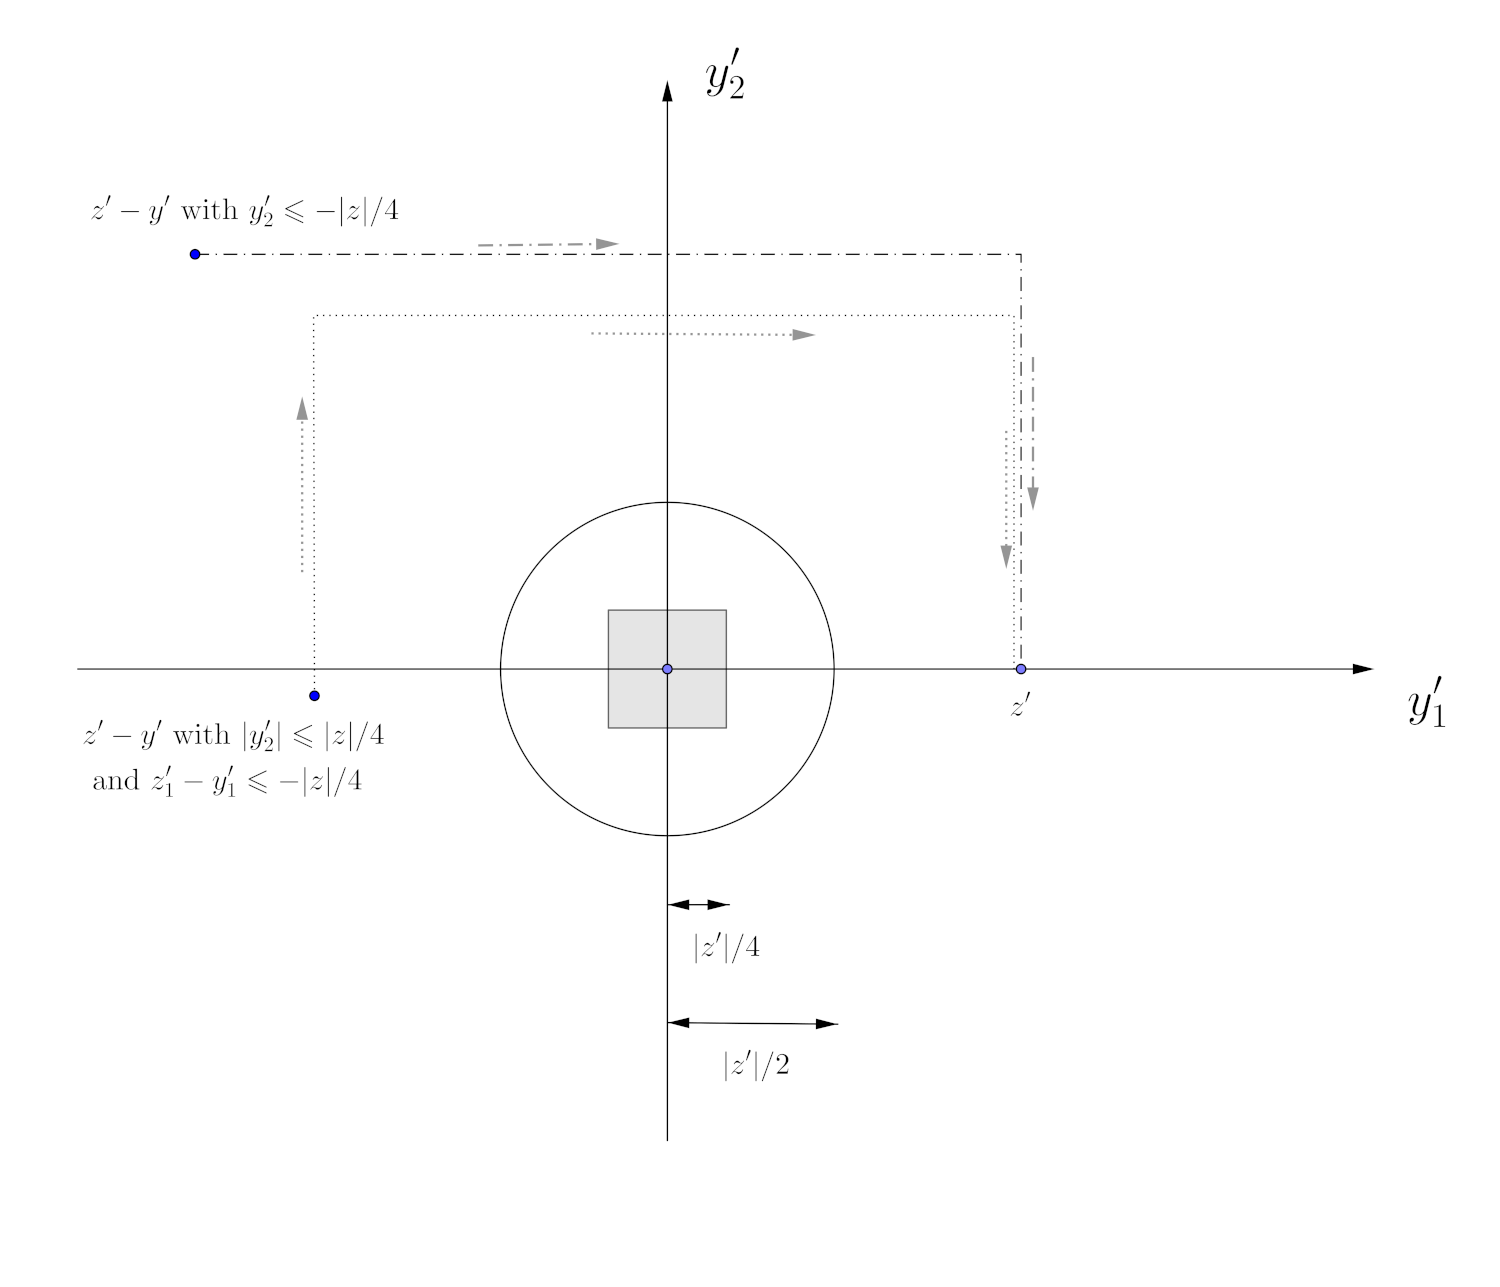
\includegraphics[scale=1.25]{path_TAF.png}
\vspace*{-50pt}
\caption{The path $ \gamma_{y,z} $}\label{fig:chemin}
\end{figure} 
The length of this path is $ \ls | y'_1 | + | y'_2 | \ls 2 |y| $ and, along this path, we have
\[
\lvert \nabla u \rvert
\ls \frac{4 \| u \|_{X^1_{\nu}} }{ |z|^{\nu+1} }
\]
(for the first part, $ | \gamma_{y,z} | \gs | (\gamma_{y,z})'_2 | = | - y'_2 | \gs |z| / 4 $, and, on the second part, $ | \gamma_{y,z} | \gs | (\gamma_{y,z})'_1 | = |z| $), hence
\begin{equation}\label{TAF}
\lvert u (z-y) - u (z) \rvert
\ls \frac{C \| u \|_{X^1_{\nu}} |y|}{ |z|^{\nu+1} }.
\end{equation}
If $ y'_2 \gs |z| / 4 $, we use the symmetric path with respect to the $ z'_1 $ axis and also get~\eqref{TAF}. If $ | y'_2 | \ls |z| / 4 $ and $ z'_1 - y'_1 \gs |z| / 4 $, the estimate~\eqref{TAF} remains true with the first path, simply noticing that, for the first part of the path, we also have $ | \gamma_{y,z} | \gs | (\gamma_{y,z})'_1 | = | z'_1 - y'_1 + t | \gs |z| / 4 $. Finally, if $ | y'_2 | \ls |z| / 4 $ and $ z'_1 - y'_1 \ls - |z| / 4 $, we follow (see the dotted line in Figure~\ref{fig:chemin}) the path $ (z'_1 - y'_1, z'_2 - y'_2) \to (z'_1 - y'_1, |z|) $ parallel to the $z'_2$-axis, then $ (z'_1 - y'_1, |z|) \to (z'_1 = |z|, |z|) $ parallel to the $z'_1$-axis, and finally $ (z'_1 = |z|, |z|)\to (z'_1 = |z|, 0) $ parallel to the $z'_2$-axis. The length of this path is $ \ls C |z| $, and, by hypothesis, $ z'_1 - y'_1 \ls - |z| / 4 \ls 0 $, thus $ |y| \gs y'_1 \gs z'_1 = |z| $, and then $ \lvert \nabla u \rvert \ls C \| u \|_{X^1_\nu} / |z|^{\nu+1} $. Therefore,
\[
\lvert u (z-y) - u (z) \rvert
\ls \frac{C \| u \|_{X^1_\nu} |z|}{ |z|^{\nu+1} }
\ls \frac{C \| u \|_{X^1_\nu} |y|}{ |z|^{\nu+1} },
\]
which proves~\eqref{TAF} in this last case. We then infer, for the third integral,
\begin{align*}
\int_{\R^2} \lvert u (z-y) & - u (z) \rvert \times \lvert v(y) \rvert \bfun_{|y|\,\ls\,2 |z| \text{ and } |z-y|\,\gs\,|z| /2 } \, dy
\\
& \ls
\frac{C \| u \|_{X^1_\nu} }{|z|^{\nu+1}}
\| v \|_{X_{\mu+1} } \int_{\R^2} \frac{ |y|}{ (1 + |y|)^{\mu+1} } \bfun_{|y|\,\ls\,2 |z| \text{ and } |z-y|\,\gs\,|z| /2 } \, dy
\\
& \ls
\frac{C}{|z|^{\nu +1}} \| u \|_{X^1_\nu} \| v \|_{X_{\mu+1} }
\int_0^{2|z|} \frac{ r^2 \, dr}{ (1 + r)^{\mu+1} }
\\
& \ls
\frac{C(\mu)}{|z|^{\mu + \nu-1 }} \| u \|_{X^1_\nu} \| v \|_{X_{\mu+1} },
\end{align*}
since $ \mu < 2 $. Gathering all these estimates, we have shown~\eqref{lemm4.1.1}.

\noindent\eqref{lemm4.1.3} For $ z \in \R^2 $ with $ |z| \gs 4 $, we have
\[
\lvert u \star v (z) \rvert
\ls \int_{D(z,2)} \lvert u (z-y) \rvert \times \lvert v (y) \rvert \, dy.
\]
Moreover, using that $ |y| \gs |z| - |z-y| \gs |z| - 2 \gs |z|/2 $, we deduce
\begin{align*}
\int_{D(z,2) } \lvert u (z-y) \rvert \times \lvert v(y) \rvert \, dy & \ls C(\mu)
\frac{ \| v \|_{X_{\mu}} }{ \lvert z \rvert^{\mu } }
\int_{D(z,2)} \lvert u (z-y) \rvert \, dy = C(\mu) \| u \|_{L^1 }
\frac{ \| v \|_{X_{\mu}} }{ \lvert z \rvert^{\mu } },
\end{align*}
as wished.
\end{proof}

%\bigbreak


We now turn to the proof of Proposition~\ref{mapp}. We fix $ \chi_0 \in \BC (\R^2) $ such that $ \chi_0 \equiv 1 $ in $ \bar{D}(0,1) $ and $ \chi_0 \equiv 0 $ outside $ \bar{D}(0,2) $. We shall then split the convolution kernel $ \p^\alpha \BK^\e $ as
\[
\p^\alpha \BK^\e = \chi_0 \p^\alpha \BK^\e + (1 - \chi_0) \p^\alpha \BK^\e.
\]

\begin{proof}[{Proof of Proposition~\ref{mapp}$\MK$\eqref{prop2.6.3}}]
For the term $ \chi_0 \p^\alpha \BK^\e \in L^1 (\R^2) $ compactly supported in $ \bar{D}(0,2) $, we apply Lemma~\ref{decay}$\MK$\eqref{lemm4.1.3} and Proposition~\ref{noyaux}$\MK$\eqref{prop2.3.2} to infer, for $ \mu > 0 $ and $ v \in X_\mu $,
\begin{multline*}
\left\|\left(\chi_0 \p_1^3 \BK^\e\right) \star v \right\|_{X_{\mu} } + \lvert \ln \e\rvert^{-1} \left\|\left(\chi_0 \p_1^2 \p_2 \BK^\e\right) \star v\right\|_{X_{\mu}}
\\  + \e \lvert \ln \e\rvert^{-1} \left\| \left(\chi_0 \p_1 \p_2^2 \BK^\e\right) \star v \right\|_{X_{\mu}} + \e^2 \lvert \ln \e\rvert^{-1} \left\|\left(\chi_0 \p_2^3 \BK^\e\right) \star v\right\|_{X_{\mu}}
\ls C(\mu) \| v \|_{X_{\mu}}.
\end{multline*}
For any $ \alpha \in \N^2 $ with $ \alpha_1 + \alpha_2 = 3 $, the term $ (1 - \chi_0) \p^\alpha \BK^\e $ belongs to $ X_3 $ by Proposition~\ref{noyaux}$\MK$\eqref{prop2.3.1}. It then follows from Lemma~\ref{decay}$\MK$\eqref{lemm4.1.1} (with $ \nu = 3 > 2 $) that, for $ 0 < \mu < 3 $,
\[
\left\| \left[(1 - \chi_0) \p^\alpha \BK^\e\right] \star v \right\|_{X_{\mu} }
\ls C (\mu) \| v \|_{X_{\mu}}.\qedhere
\]
\end{proof}

\begin{proof}[{Proof of Proposition~\ref{mapp}$\MK$\eqref{prop2.6.2}}]
The estimates for the local term $ \chi_0 \p^\alpha \BK^\e $ (with $ \alpha_1 + \alpha_2 = 2 $) and for the term $ (1-\chi_0) \p^\alpha \BK^\e \in X_2 $ (with $ \nu = 2 $) follow as for $ (iv) $.
\end{proof}

\begin{proof}[{Proof of Proposition~\ref{mapp}$\MK$\eqref{prop2.6.1}}]
The estimate for the local term $ \chi_0 \nabla \BK^\e $ follows as for $ (iv) $. For the term $ (1-\chi_0) \nabla \BK^\e \in X_1^1 $, we apply Lemma~\ref{decay}$\MK$\eqref{lemm4.1.2} (with $ \nu = 1 < 2 $) and deduce from Proposition~\ref{noyaux}$\MK$\eqref{lemm4.1.2} that, for $ 1 < \mu < 2 $ and $ v \in X_{\mu +1,a} $,
\[
\left\|\left[(1 - \chi_0) \nabla \BK^\e\right] \star v \right\|_{X_{\mu} }
\ls C (\mu) \left\| (1 - \chi_0) \nabla \BK^\e \right\|_{X^1_1} \| v \|_{X_{\mu+1}}
\ls C (\mu) \| v \|_{X_{\mu+1 }}.\qedhere
\]
\end{proof}

\begin{proof}[{Proof of Proposition~\ref{mapp}$\MK$\eqref{prop2.6.2'}}]
The estimate for the local terms $ \chi_0 \nabla^2 \BK^\e $ follows as for $ (iv) $. For the terms $ (1-\chi_0) \nabla^2 \BK^\e \in X_2^1 $, we apply Proposition~\ref{noyaux}$\MK$\eqref{prop2.3.1} and Lemma~\ref{decay}$\MK$\eqref{lemm4.1.2} (with $ "\mu" = \mu - 1 \in]1,2[$ and $ "\nu" = 2 + \mu' - \mu \in [0, 2 [$, so that $ "\mu" + "\nu" - 1 = \mu' $) and deduce, for $ v \in X_{\mu, a} $,
\[
\left\|\left[(1 - \chi_0) \nabla^2 \BK^\e\right] \star v\right\|_{X_{ \mu' } }
\ls C (\mu, \mu') \left\| (1 - \chi_0) \nabla^2 \BK^\e \right\|_{X^1_{2 + \mu' - \mu }} \| v \|_{X_{\mu}}
\ls C (\mu, \mu') \| v \|_{X_{\mu}}.\qedhere
\]
\end{proof}


\subsection{Proof of Proposition~\ref{esti-noyau-infini}}

Let us first prove the claimed estimates on $ (A, \phi) $ given by~\eqref{sol_eq_infini}. It is easy to check that all the terms are well-defined thanks to the decays imposed on $ \BS_{\amm} $ and $ \BS_{\phl} $.

\noindent\emph{Estimate for $ A $.} By Proposition~\ref{mapp}$\MK$\eqref{prop2.6.2}, we have
\[
\left\| \p_2^2 \BK^\e \star \BS_{\amm} \right\|_{ X_{1 + \s} }
\ls C(\s,\s') \lne^2 \| \BS_{\amm} \|_{ X_{1 + \s'} }
\]
and, by Proposition~\ref{mapp}$\MK$\eqref{prop2.6.1}, since $ \BS_{\phl} $ is odd in $ z_1 $, thus has vanishing integral,
\[
\left\| \p_1 \BK^\e \star \BS_{\phl} \right\|_{ X_{1 + \s} }
\ls C(\s, \s') \| \BS_{\phl} \|_{ X_{ 2 + \s'} }.
\]
Therefore, using $ c(\e) = \cs + \BO(\e^2) $,
\[
\| A \|_{X_{1+\s}} \ls \| \BT \|_{ X_{1+\s}} + C(\s, \s') \lne^2 \| \BS_{\amm} \|_{ X_{1 + \s'} } + C(\s, \s') \| \BS_{\phl} \|_{ X_{ 2 + \s' } },
\]
with
\begin{align*}
\BT = \e^{-2} \left(\p_1^2 \BK^\e \star \BS_{\amm} - \cs \p_1 \BK^\e \star \BS_{\phl}\right) =
\e^{-2} \p_1^2 \BK^\e \star (\BS_{\amm} - \cs \BI \BS_{\phl}),
\end{align*}
hence, by Proposition~\ref{mapp}$\MK$\eqref{prop2.6.1},
\[
\e^2 \| \BT \|_{X_{1+\s}} \ls C(\s, \s') \| \BS_{\amm} - \cs \BI \BS_{\phl} \|_{ X_{1 + \s' } }.
\]
If $ \BS_{\amm} = 0 $, then we may write, by Proposition~\ref{mapp}$\MK$\eqref{prop2.6.1} ($ \BS_{\phl}$ is odd in $ z_1 $, thus has vanishing integral),
\[
\e^2 \| \BT \|_{X_{1+\s}} = \cs \left\| \p_1 \BK^\e \star \BS_{\phl}\right\|_{X_{1+\s}}
\ls C(\s, \s') \| \BS_{\phl} \|_{ X_{2 + \s' } }.
\]

\noindent\emph{Estimate for $ \nabla \phi $.} By Proposition~\ref{mapp}$\MK$\eqref{prop2.6.2} and~\eqref{prop2.6.3}, we have
\begin{align*}
\left\| \nabla \p_1 \BK^\e \star \BS_{\amm} \right\|_{ X_{1 + \s} }
&\ls C(\s, \s') \| \BS_{\amm} \|_{ X_{1 + \s'} }
\\
\intertext{and}
\left\| \nabla \p_1^2 \BK^\e \star \BS_{\phl} \right\|_{ X_{1 + \s} } + \e^2 \left\| \nabla \p_2^2 \BK^\e \star \BS_{\phl} \right\|_{ X_{1 + \s} }
&\ls C(\s, \s') \lne^2 \left\| \BS_{\phl} \right\|_{ X_{1 + \s'} }.
\end{align*}
Therefore, using $ c(\e) = \cs + \BO(\e^2) $,
\[
\| \nabla \phi \|_{X_{1+\s}}
\ls \| \BT \|_{ X_{1+\s}} + C(\s, \s') \| \BS_{\amm} \|_{ X_{1 + \s'} } + C(\s, \s') \lne^2 \| \BS_{\phl} \|_{ X_{ 1 + \s' } },
\]
with
\begin{align*}
\BT = \frac{\cs}{ \e^{2} } \left(\nabla \p_1 \BK^\e \star \BS_{\amm} - \cs \nabla \BK^\e \star \BS_{\phl}\right) = \frac{\cs}{ \e^{2} } \nabla \p_1 \BK^\e \star \left(\BS_{\amm} - \cs \BI \BS_{\phl}\right),
\end{align*}
hence, by Proposition~\ref{mapp}$\MK$\eqref{prop2.6.2},
\[
\e^2 \| \BT \|_{X_{1+\s}}
\ls C(\s, \s') \left\| \BS_{\amm} - \cs \BI \BS_{\phl} \right\|_{ X_{1 + \s' } }.
\]
If $ \BS_{\amm} = 0 $, then we may write, by Proposition~\ref{mapp}$\MK$\eqref{prop2.6.1} ($\BS_{\phl} $ is odd in $ z_1$),
\[
\e^2 \| \BT \|_{X_{1+\s}} = \cs \| \nabla \BK^\e \star \BS_{\phl} \|_{X_{1+\s}}
\ls C(\s, \s') \| \BS_{\phl} \|_{ X_{2 + \s' } }.
\]
Combining these two estimates, we infer
\begin{align*}
\| A \|_{X_{1+\s}} + \| \nabla \phi \|_{ X_{1+\s}} & \ls C(\s, \s') \lne^2 \left(\| \BS_{\phl} \|_{ X_{ 2 + \s' } } + \| \BS_{\amm} \|_{ X_{1 + \s' } }\right)
\\ & \quad + \frac{C(\s, \s')}{\e^2} \| \BS_{\amm} - \cs \BI \BS_{\phl} \|_{ X_{1 + \s' } },
\end{align*}
and, when $ \BS_{\amm} = 0 $, we have
\begin{multline*}
\| A \|_{X_{1+\s}} + \| \nabla \phi \|_{ X_{1+\s}} \\ \ls C(\s, \s') \| \BS_{\amm} \|_{ X_{1 + \s' } } + C(\s, \s') \lne^2 \| \BS_{\phl} \|_{ X_{ 2 + \s' } }
 + \frac{C(\s, \s')}{\e^2} \| \BS_{\phl} \|_{ X_{1 + \s' } }.
\end{multline*}

\noindent \emph{Estimate for $ \nabla A $.} By Proposition~\ref{mapp}$\MK$\eqref{prop2.6.2'}, we have, since $ \int \nabla \BS_{\amm} \, dz = 0 $,
\[
\left\| \p_2^2 \BK^\e \star \nabla \BS_{\amm}\right\|_{ X_{2 + \s} }
\ls C(\s, \s') \lne^2 \left\| \nabla \BS_{\amm} \right\|_{ X_{2 + \s' } }
\]
and, since $ \BS_{\phl} \in X_{2 + \s, a } $ has also vanishing integral,
\[
\left\| \nabla \p_1 \BK^\e \star \BS_{\phl} \right\|_{ X_{2 + \s} }
\ls C (\s, \s') \left\| \BS_{\phl} \right\|_{ X_{ 2 + \s' } }.
\]
Therefore, using $ c(\e) = \cs + \BO(\e^2) $,
\[
\| \nabla A \|_{X_{2+\s }}
\ls \| \BT \|_{X_{2 +\s}} + C(\s,\s') \lne^2 \| \nabla \BS_{\amm} \|_{ X_{2 + \s' } } + C(\s, \s') \| \BS_{\phl} \|_{ X_{ 2 + \s' } },
\]
with
\begin{align*}
\BT = \e^{-2} \nabla \left(\p_1^2 \BK^\e \star \BS_{\amm} - \cs \p_1 \BK^\e \star \BS_{\phl}\right) =
\e^{-2} \p_1^2 \BK^\e \star \nabla (\BS_{\amm} - \cs \BI \BS_{\phl}),
\end{align*}
hence, by Proposition~\ref{mapp}$\MK$\eqref{prop2.6.2'} (since $ \int \nabla (\BS_{\amm} - \cs \BI \BS_{\phl}) \, dz = 0 $),
\[
\e^2 \| \BT \|_{X_{2+\s}}
\ls C(\s, \s') \left\| \nabla\left(\BS_{\amm} - \cs \BI \BS_{\phl}\right) \right\|_{ X_{2 + \s' } }.
\]
If $ \BS_{\amm} = 0 $, then, by Proposition~\ref{mapp}$\MK$\eqref{prop2.6.2'}, ($\BS_{\phl}$ is odd in $z_1 $), we may write
\[
\e^2 \| \BT \|_{X_{2+\s}} = \cs \left\| \nabla \p_1 \BK^\e \star \BS_{\phl} \right\|_{X_{2+\s}}
\ls C(\s, \s') \| \BS_{\phl} \|_{ X_{2 + \s' } }.
\]

\noindent \emph{Estimate for $ \nabla^2 \phi $.} Let $ j$, $k \in \{ 1, 2 \} $. By Proposition~\ref{mapp}$\MK$\eqref{prop2.6.2'} ($ \int \p_k \BS_{\amm} \, dz = 0 $) and~\eqref{prop2.6.3}, we have
\begin{align*}
\left\| \p_j \p_k \left(\p_1 \BK^\e \star \BS_{\amm}\right) \right\|_{ X_{2 + \s} } = \left\| \p_j \p_1 \BK^\e \star \p_k \BS_{\amm} \right\|_{ X_{2 + \s} }
&\ls C(\s, \s') \left\| \nabla \BS_{\amm} \right\|_{ X_{2 + \s' } }
\\
\intertext{and}
\left\| \p_j \p_1^2 \BK^\e \star \p_k \BS_{\phl} \right\|_{ X_{2 + \s} } + \e^2 \left\| \p_j \p_2^2 \BK^\e \star \p_k \BS_{\phl} \right\|_{ X_{2 + \s} }
&\ls C(\s, \s') \lne^2 \left\| \nabla \BS_{\phl} \right\|_{ X_{2 + \s' } }.
\end{align*}
Therefore, using $ c(\e) = \cs + \BO(\e^2) $,
\[
\left\| \p_j \p_k \phi \right\|_{ X_{2+\s}}
\ls \| \BT \|_{ X_{2+\s}} + C(\s, \s') \| \nabla \BS_{\amm} \|_{ X_{2 + \s' } } + C(\s, \s') \lne^2 \| \nabla \BS_{\phl} \|_{ X_{ 2 + \s ' } },
\]
with
\begin{align*}
\BT = \frac{\cs}{ \e^{2} } \p_j \p_k \left(\p_1 \BK^\e \star \BS_{\amm} - \cs \BK^\e \star \BS_{\phl}\right) = \frac{\cs}{ \e^{2} } \p_j \p_1 \BK^\e \star \p_k \left(\BS_{\amm} - \cs \BI \BS_{\phl}\right),
\end{align*}
hence, by Proposition~\ref{mapp}$\MK$\eqref{prop2.6.2'} ($ \p_k (\BS_{\amm} - \cs \BI \BS_{\phl}) $ has zero integral),
\[
\e^2 \| \BT \|_{ X_{2+\s}}
\ls C(\s,\s') \left\| \nabla \left(\BS_{\amm} - \cs \BI \BS_{\phl}\right) \right\|_{ X_{2 + \s' } }.
\]
If $ \BS_{\amm} = 0 $, then we may write, by Proposition~\ref{noyaux}$\MK$\eqref{prop2.6.2'}($ \BS_{\phl}$ is odd in $z_1$, thus has vanishing integral),
\[
\e^2 \| \BT \|_{X_{2+\s}} = \cs \left\| \p_j\p_k \BK^\e \star \BS_{\phl} \right\|_{X_{2+\s}}
\ls C(\s, \s') \lne^2 \| \BS_{\phl} \|_{ X_{2 + \s' } }.
\]

Combining these two estimates, we infer
\begin{align*}
\| \nabla A \|_{ X_{2+\s}} + \left\| \nabla^2 \phi \right\|_{ X_{2+\s}} & \ls C(\s,\s') \lne^2 \Big(\left\| \BS_{\amm} \right\|_{ X^{1}_{ 1 + \s'} } + \left\| \BS_{\phl} \right\|_{ X^{ 1}_{ 2 + \s' } } \Big)
\\ & \quad + \frac{C(\s, \s')}{\e^2} \left\| \BS_{\amm} - \cs \BI \BS_{\phl} \right\|_{ X^{1}_{ 1 + \s' } },
\end{align*}
and when $ \BS_{\amm} = 0 $, then we have
\[
\| \nabla A \|_{ X_{2+\s}} + \left\| \nabla^2 \phi \right\|_{ X_{2+\s}}
\ls C(\s,\s') \lne^2 \| \BS_{\phl} \|_{ X^{ 1}_{ 2 + \s' } } + \frac{C(\s, \s')}{\e^2} \lne \| \BS_{\phl} \|_{ X_{ 1 + \s' } }.
\]



\noindent\emph{Estimate for $ \nabla^2 A $.} We start with estimating $ \p_1^2 A $. By Proposition~\ref{mapp}$\MK$\eqref{prop2.6.3}, we have,
\begin{align*}
\left\| \p_1^2 \p_2^2 \left(\BK^\e \star \BS_{\amm}\right) \right\|_{ X_{2 + \s} } = \left\| \p_1^2 \p_2 \BK^\e \star \p_2 \BS_{\amm} \right\|_{ X_{2 + \s} }
&\ls C(\s, \s') \lne^2 \left\| \nabla \BS_{\amm} \right\|_{ X_{2 + \s' } }
\\
\intertext{and}
\left\| \p_1^2 \p_1 \BK^\e \star \BS_{\phl} \right\|_{ X_{2 + \s} }
&\ls C (\s, \s') \| \BS_{\phl} \|_{ X_{ 2 + \s' } }.
\end{align*}
Therefore, using $ c(\e) = \cs + \BO(\e^2) $,
\[
\left\| \p_1^2 A \right\|_{X_{2+\s }}
\ls \| \BT \|_{X_{2 +\s}} + C(\s,\s') \lne^2 \left\| \nabla \BS_{\amm}\right\|_{ X_{2 + \s' } } + C(\s, \s') \left\| \BS_{\phl}\right\|_{ X_{ 2 + \s' } },
\]
with
\begin{align*}
\BT = \e^{-2} \p_1^2 \left(\p_1^2 \BK^\e \star \BS_{\amm} - \cs \p_1 \BK^\e \star \BS_{\phl}\right) =
\e^{-2} \p_1^3 \BK^\e \star \p_1 \left(\BS_{\amm} - \cs \BI \BS_{\phl}\right),
\end{align*}
hence, by Proposition~\ref{mapp}$\MK$\eqref{prop2.6.3},
\[
\e^2 \| \BT \|_{X_{2+\s}}
\ls C(\s, \s') \| \nabla(\BS_{\amm} - \cs \BI \BS_{\phl}) \|_{ X_{2 + \s' } }.
\]
If $ \BS_{\amm} = 0 $, then we may write
\[
\e^2 \| \BT \|_{X_{2+\s}} = \cs \left\| \p_1^3 \BK^\e \star \BS_{\phl} \right\|_{X_{2+\s}}
\ls C(\s, \s') \| \BS_{\phl} \|_{ X_{2 + \s' } }.
\]
This gives, as wished, the estimate for $ \p_1^2 A $ in $ X_{2+\s } $.

We then consider $ \p_1 \p_2 A $. By Proposition~\ref{mapp}$\MK$\eqref{prop2.6.3}, we have, since $ \nabla \BS_{\amm} \in X_{2 + \s' } $ has zero integral,
\begin{align*}
\left\| \p_1 \p_2^3 \left(\BK^\e \star \BS_{\amm}\right) \right\|_{ X_{2 + \s} } = \left\| \p_1 \p_2^2 \BK^\e \star \p_2 \BS_{\amm} \right\|_{ X_{2 + \s} }
&\ls C(\s, \s') \frac{ \lne}{\e} \left\| \nabla \BS_{\amm} \right\|_{ X_{2 + \s' } }
\\
\intertext{and, since $ \p_2 \BS_{\phl} \in X_{2 + \s, 0 }, $}
\left\| \p_2 \p_1^2 \BK^\e \star \BS_{\phl} \right\|_{ X_{2 + \s} } = \left\| \p_1^2 \BK^\e \star \p_2 \BS_{\phl} \right\|_{ X_{2 + \s} }
&\ls C (\s, \s') \left\| \nabla \BS_{\phl} \right\|_{ X_{ 2 + \s' } }.
\end{align*}
Therefore, using $ c(\e) = \cs + \BO(\e^2) $,
\[
\left\| \p_1 \p_2 A \right\|_{X_{2+\s }}
\ls \| \BT \|_{X_{2 +\s}} + C(\s,\s') \frac{\lne}{\e} \| \nabla \BS_{\amm} \|_{ X_{2 + \s' } } + C(\s, \s') \left\| \nabla \BS_{\phl} \right\|_{ X_{ 2 + \s' } },
\]
with
\begin{align*}
\BT = \e^{-2} \p_1 \p_2 \left(\p_1^2 \BK^\e \star \BS_{\amm} - \cs \p_1 \BK^\e \star \BS_{\phl}\right) =
\e^{-2} \p_1^3 \BK^\e \star \p_2 \left(\BS_{\amm} - \cs \BI \BS_{\phl}\right),
\end{align*}
hence, by Proposition~\ref{mapp}$\MK$\eqref{prop2.6.3},
\[
\e^2 \| \BT \|_{X_{2+\s}}
\ls C(\s, \s') \left\| \nabla\left(\BS_{\amm} - \cs \BI \BS_{\phl}\right) \right\|_{ X_{2 + \s' } }.
\]
If $ \BS_{\amm} = 0 $, then we may write ($\int \p_1 \BS_{\phl} \, dz = 0 $)
\[
\e^2 \| \BT \|_{X_{2+\s}}
\ls C(\s, \s') \left\| \p_1 \p_2 \BK^\e \star \p_1 \BS_{\phl} \right\|_{X_{2+\s}}
\ls C(\s, \s') \left\| \p_1 \BS_{\phl} \right\|_{X_{2 + \s'}}.
\]
This gives the desired estimate for $ \p_1 \p_2 A $ in $ X_{2+\s } $.

We finally consider $ \p_2^2 A $. By Proposition~\ref{mapp}$\MK$\eqref{prop2.6.3}, we have
\[
\left\| \p_2^4 \left(\BK^\e \star \BS_{\amm}\right) \right\|_{ X_{2 + \s} } = \left\| \p_2^3 \BK^\e \star \p_2 \BS_{\amm} \right\|_{ X_{2 + \s} }
\ls C(\s, \s') \frac{ \lne}{\e^2} \| \nabla \BS_{\amm} \|_{ X_{2 + \s' } }
\]
and, by Proposition~\ref{mapp}$\MK$\eqref{prop2.6.2'} ($ \int \p_2 \BS_{\phl} \, dz = 0 $),
\[
\left\| \p_2^2 \p_1 \BK^\e \star \BS_{\phl} \right\|_{ X_{2 + \s} } = \left\| \p_1 \p_2 \BK^\e \star \p_2 \BS_{\phl}\right\|_{ X_{2 + \s} }
\ls C (\s, \s') \left\| \nabla \BS_{\phl} \right\|_{ X_{ 2 + \s' } }.
\]
Therefore, using $ c(\e) = \cs + \BO(\e^2) $,
\[
\left\| \p_2^2 A \right\|_{X_{2+\s }}
\ls \| \BT \|_{X_{2 +\s}} + C(\s,\s') \frac{\lne }{\e^2 } \left\| \nabla \BS_{\amm} \right\|_{ X_{2 + \s' } } + C(\s, \s') \left\| \nabla \BS_{\phl} \right\|_{ X_{ 2 + \s' } },
\]
with
\begin{align*}
\BT = \e^{-2} \p_2^2 \left(\p_1^2 \BK^\e \star \BS_{\amm} - \cs \p_1 \BK^\e \star \BS_{\phl}\right) =
\e^{-2} \p_2 \p_1^2 \BK^\e \star \p_2 \left(\BS_{\amm} - \cs \BI \BS_{\phl}\right),
\end{align*}
hence, by Proposition~\ref{mapp}$\MK$\eqref{prop2.6.3},
\[
\e^2 \| \BT \|_{X_{2+\s}}
\ls C(\s, \s') \lne^2 \left\| \nabla\left(\BS_{\amm} - \cs \BI \BS_{\phl}\right) \right\|_{ X_{2 + \s' } }.
\]
If $ \BS_{\amm} = 0 $, then we may write, by Proposition~\ref{mapp}$\MK$\eqref{prop2.6.2'}($ \int \p_2 \BS_{\phl} \, dz = 0 $),
\[
\e^2 \| \BT \|_{X_{2+\s}} = \cs \left\| \p_1 \p_2 \BK^\e \star \p_2 \BS_{\phl} \right\|_{X_{2+\s}}
\ls C(\s, \s') \left\| \p_1 \BS_{\phl} \right\|_{ X_{2 + \s' } }.
\]
This gives the required estimate for $ \p_2^2 A $ in $ X_{2+\s } $.



\begin{rema}
It may be noticed that the proof does not require $ \nabla \BS_{\phl} \in X_{3 + \s' } $, but only $ \nabla \BS_{\phl} \in X_{2 + \s' } $. We shall not need this information during the proof.
\end{rema}



Let us now turn to the uniqueness part. By using Fourier transform in the sense of tempered distributions, we see that~\eqref{sol_eq_infini} is indeed a solution of the system~\eqref{eq_infini}. We now consider $ (A, \phi) $ solution of the homogeneous problem
\begin{equation*}
\left\{
\begin{array}{ll}
\ds{ c(\e) \p_{1} A - \left(\p_{1}^2 + \e^2 \p^2_{2}\right) \phi = 0 }\\ \ \\
\ds{ - c(\e) \p_{1} \phi + \left(\cs^2 - \e^2\left(\p_{1}^2 + \e^2 \p_{2}^2\right)\right) A = 0.}
\end{array}\right.
\end{equation*}
By taking Fourier transform and combining the two equations, we infer
\[
\Big(\xi_1^2 + \cs^2 \xi_2^2 + \left(\xi_1^2 + \e^2 \xi_2^2\right)^2 \Big) \Fou(A) = \Big(\xi_1^2 + \cs^2 \xi_2^2 + \left(\xi_1^2 + \e^2 \xi_2^2\right)^2 \Big) \Fou(\phi) = 0.
\]
Since the symbol $ \xi_1^2 + \cs^2 \xi_2^2 + (\xi_1^2 + \e^2\xi_2^2)^2 $ vanishes only at the origin, a classical result due to L. Schwartz asserts that $ \Fou(A) $ and $ \Fou(\phi) $ are linear combination of Dirac masses at the origin and their derivatives, which means that $ A $ and $ \phi $ are polynomial functions. Since $ A \in X_{1+\s} $, the only possibility is $A \equiv 0 $. Concerning $ \phi $, we only have $ \nabla \phi \in X_{1+\s} $, which imposes that $ \phi $ is constant in $ \R^2 $, and since it is assumed odd in $ z_1 $, we deduce $ \phi \equiv 0 $, as wished.



\subsection{Proof of Proposition~\ref{esti-apriori}}



\subsubsection{A priori estimate in the plane}

We first establish an a priori estimate on the solutions to~\eqref{Mad_lineaire} (assuming existence).


\begin{lemm}\label{esti-apriori_plan}
Let $ 0 < \s < \s' < 1 $ be given. Then, there exists $ \ep (\s, \s') \in]0,1[$ and $ C (\s,\s') > 0 $ such that, for any $ 0 < \e < \ep(\s, \s') $, any $ (\BS_{\phl}, \BS_{\amm}) \in X^{1}_{2+\s', a} \times X^{1}_{1+\s', s} $ and any $ (A, \nabla \phi) \in X^{1}_{ 1+\s'} \times X^{1}_{ 1+ \s'} $, satisfying the linear system~\eqref{Mad_lineaire}, namely
\begin{equation*}
\left\{
\begin{array}{ll}
c(\e) \p_{1} A -\left(\p_{1}^2 + \e^2 \p^2_{2}\right) \phi - 2 \e^2 \p_{1} \phi \p_{1} A^{(0)} - 2 \e^4 \p_{2} \phi \p_{2} A^{(0)}
\\
\quad - \e^2 c(\e) \p_1 (A^{(0)} A) + 2 \e^2 \p_{1} \phi^{(0)} \p_{1} A = \BS_{\phl} \\ \ \\
- c(\e) \p_{1} \phi - \e^2 c(\e) A^{(0)} \p_1 \phi - \e^2 c(\e) A \p_1 \phi^{(0)} + 2 \e^2 \p_{1} \phi^{(0)} \p_{1} \phi + \cs^2 A
\\
\quad - \e^2 \cs^2 (\Gamma -3) A^{(0)} A - \e^2 \left(\p_{1}^2 A + \e^2 \p_{2}^2 A\right) = \BS_{\amm},
\end{array}\right.
\end{equation*}
then we have
\begin{align*}
\| A \|_{ X^1_{ 1+ \s} } & + \| \nabla \phi \|_{ X^1_{1+ \s} }
\\ & \ls C (\s, \s') \lne^2
\left(
\left\| \BS_{\phl} \right\|_{ X^{1}_{ 2+\s } } + \left\| \BS_{\amm} \right\|_{ X^{ 1}_{1+\s} } + \frac{1}{\e^2} \left\| \cs \BI \BS_{\phl} - \BS_{\amm} \right\|_{ X^{1}_{1+\s'}}
\right).
\end{align*}
\end{lemm}

\begin{proof} 
We argue by contradiction and assume that there exist sequences $ (\e_n)_{n\,\in\,\N} $ tending to $0$, $ (\BS_{{\phl},n}, \BS_{{\amm},n}) \in X^1_{2+\sigma} \times X^1_{1+ \sigma'} $ and $ (\phi_n, A_n) \in \dot{X}^1_{1+\s} \times X^1_{1+\s} $, satisfying~\eqref{Mad_lineaire}, that is
\begin{equation}\label{syst_absurde}
\left\{
\begin{array}{ll}
c (\e_n) \p_{1} A_n - \left(\p_{1}^2 + \e_n^2 \p^2_{2}\right) \phi_n - 2 \e_n^2 \p_{1} \phi_n \p_{1} A^{(0)} - 2 \e_n^4 \p_{2} \phi_n \p_{2} A^{(0)}
\\
\quad - \e_n^2 c(\e_n) \p_1 \left(A^{(0)} A_n\right) + 2 \e_n^2 \p_{1} \phi^{(0)} \p_{1} A_n = \BS_{{\phl},n} \\ \ \\
- c(\e_n) \p_{1} \phi_n - \e_n^2 c (\e_n) A^{(0)} \p_1 \phi_n - \e_n^2 c(\e_n) A_n \p_1 \phi^{(0)} + 2 \e_n^2 \p_{1} \phi^{(0)} \p_{1} \phi_n
\\
\quad + \cs^2 A_n + \e_n^2 \cs^2 (\Gamma -3) A^{(0)} A_n - \e_n^2 \left(\p_{1}^2 A_n + \e_n^2 \p_{2}^2 A_n\right) = \BS_{{\amm},n},
\end{array}\right.
\end{equation}
such that
\begin{equation}\label{hypoth1}
\| A_n \|_{ X^1_{ 1+\s} } + \| \nabla \phi_n \|_{ X^1_{ 1 +\s} } + \left\| \left(\p_1^2 A_n, \e_n \p_1\p_2 A_n, \e_n^2 \p_2^2 A_n \right)\right\|_{ X_{ 2+\s} } = 1
\end{equation}
and
\begin{equation}\label{hypoth2}
\lvert \ln \e_n \rvert^2 \left(\left\| \BS_{{\phl},n} \right\|_{ X^1_{2+\s', a} } + \left\| \BS_{{\amm},n} \right\|_{ X^1_{1+\s'} } + \frac{1}{\e_n^2} \left\| c \BI \BS_{{\phl},n} - \BS_{{\amm},n} \right\|_{ X^1_{1+\s'} }
\right)
\to 0.
\end{equation}

%\noindent\emph{Step 1: Local convergence.} 
\begin{step}{{Local convergence}}\label{step1sect4.4}
First, we notice that since $ \phi_n $ is odd in $ z_1 $, we have $ \phi(0, z_2) = 0 $ for any $ z_2 \in \R $, and this implies, for $ z_1 \in \R_+ $, $z_2 \in \R $,
\begin{align*}
\lvert \phi_n (z_1, z_2) \rvert
\ls \int_0^{z_1} \lvert \p_1 \phi_n (\zeta, z_2) \rvert \, d\zeta & \ls \| \nabla \phi_n \|_{X_{1+\s}} \int_0^{z_1} \frac{d\zeta }{ (1 + |(\zeta, z_2) |)^{1+\s} }
\\ & \ls C(\s) \| \nabla \phi_n \|_{X_{1+\s}}.
\end{align*}
By Ascoli's Theorem, we may assume, up to a subsequence, that there exists $ (A_\ii, \phi _\ii) \in X^1_{1+\s} $ such that
\[
A_n \to A_\ii
\qquad 
\phi_n \to \phi_\ii
\qquad
\nabla \phi_n \to \nabla \phi_\ii
\qquad
\text{strongly in } \BC^0_{\locc} (\R^2).
\]
In view of the bounds $ \| A_n \|_{ X_{ 1+\s} } + \| \nabla \phi_n \|_{ X_{ 1 +\s} } \ls 1 $, we actually have
\[
A_n \to A_\ii
\qquad
\nabla \phi_n \to \nabla \phi_\ii
\qquad
\text{strongly in } \BC_{b} (\R^2).
\]
Furthermore, we may assume that $ (\nabla A_n)_{n\,\in\,\N}$ is weakly convergent in $ L^2 $. The weak limit can only be $ \nabla A_\ii $ since $ A_n \to A_\ii $ in $ \BC^0_{\locc} (\R^2) $. Arguing in a similar way, we may then assume
\[
\nabla A_n \rightharpoonup \nabla A_\ii,
\quad \quad
\p_1^2 A_n \rightharpoonup \p_1^2 A_\ii
\quad \quad
\nabla^2 \phi_n \rightharpoonup \nabla^2 \phi_\ii
\quad \quad
\text{weakly in } L^2 (\R^2).
\]

In view of the bounds~\eqref{hypoth1} and~\eqref{hypoth2}, we may easily pass to the (weak, or distributional) limit in~\eqref{syst_absurde} and get
\[
\left\{
\begin{array}{ll}
- \cs \p_{1} A_\ii + \p_{1}^2 \phi_\ii = 0 \\ \ \\
\cs \p_{1} \phi_\ii - \cs^2 A_\ii = 0,
\end{array}\right.
\]
that is the preparedness relation
\[
\cs A_\ii = \p_{1} \phi_\ii.
\]

As for the derivation of the KP-I solitary wave equation, we now subtract $ c(\e_n) / \cs^2 $ times the first equation of~\eqref{Mad_lineaire} and $
\p_{1}/\cs^2 $ times the second one. This gives
\begin{multline}\label{desing_lineaire}
\frac{\cs^2 - c^2(\e_n) }{\e_n^2 \cs^2} \p_{1} A_n - \frac{1}{\cs^2} \p_{1} \left(\p_{1}^2 A_n + \e_n^2 \p_2^2 A_n\right) + \frac{c(\e_n) }{ \cs^2} \p_2^2 \phi_n\\
\begin{aligned}
& +
\left\{ 2 \frac{c(\e_n)}{\cs^2} \p_{1} \phi^{(0)} \p_{1} A_n + 2 \frac{c(\e_n)}{\cs^2} \p_{1} \phi_n \p_{1} A^{(0)} + \frac{c(\e_n)^2}{\cs^2} \p_1 (A^{(0)} A_n)\right.\\
& \quad \quad - \frac{c(\e_n)}{\cs^2} \p_1 \left(A^{(0)} \p_{1} \phi_n\right) - \frac{c(\e_n)}{\cs^2} \p_1 \left(A_n \p_{1} \phi^{(0)}\right)\\
& \quad \quad\left. + \frac{2}{\cs^2} \p_{1} \left[\p_{1} \phi_n \p_{1} \phi^{(0)}\right] + (\Gamma - 3) \p_{1} \left(A_n A^{(0)}\right) \right\}
\\ & = - \frac{1}{\e_n^2 \cs^2} \p_{1} \left(\cs \BI \BS_{{\phl},n} - \BS_{{\amm},n}\right) + \frac{ \cs -c(\e_n) }{\e_n^2 \cs^2} \BS_{{\phl},n} - 2 \e_n^2 \p_{2} \phi_n \p_{2} A^{(0)}\,.
\end{aligned}
\end{multline}
Since $\cs^2 - c^2(\e_n) = \e_n^2 $, it then follows that $ A_\ii = \p_{1} \phi_\ii /\cs $ solves, in the distributional sense, the linearized KP-I solitary waves equation
\begin{equation}\label{SW_lineaire}
\frac{1}{\cs^2} \p_{1} A_\ii - \frac{1}{\cs^2} \p^3_{1} A_\ii + \G \p_{1} \left(A_\ii A^{(0)}\right) + \p_{2}^2 \p_{1}^{-1} A_\ii = 0.
\end{equation} By the result in~\cite[ Theorem~\ref{Lump_nondege}]{Liu_Wei_Lump}, we deduce that
\[
A_\ii \in \Span \left(\p_1 A^{(0)}, \p_2 A^{(0)}\right).
\]
Furthermore, we have imposed the symmetries $ A_n $ even in $z_1 $ and in $ z_2 $, whereas $ \p_1 A^{(0)} $ is odd in $z_1 $ and even in $ z_2 $, and $ \p_2 A^{(0)} $ is even in $ z_1 $ and odd in $z_2 $. It then follows that
\[
A_\ii \equiv 0,
\qquad
\phi_\ii \equiv 0,
\]
since $\phi_\ii $ is odd in $ z_1 $.
\end{step}


%\emph{Step 2: .}
\begin{step}{{Smallness in $ L^2 $}}\label{step2sect4.4}
We multiply the first equation of~\eqref{syst_absurde} by $ \phi_n $ and integrate over $ \R^2 $ by parts:
\begin{multline}\label{apriori_1}
 \int \lvert \nabla^{\e_n} \phi_n \rvert^2 - c(\e_n) A_n \p_1 \phi_n \, dz\\
 = \int \Big(\BS_{{\phl},n} \phi_n + 2 \e_n^2 \p_1 \phi^{(0)} \p_1 A_n \phi_n + 2 \e_n^2 \p_1 \phi_n \p_1 A^{(0)} \phi_n
\\
- 2 \e_n^4 \p_{2} \phi_n \p_{2} A^{(0)} \phi_n - \e_n^2 c(\e_n) A^{(0)} A_n \p_1 \phi_n \Big) \, dz.
\end{multline}
Here, we have set $ \nabla^\e = (\p_1, \e \p_2)^T $. We notice that
\[
\left\lvert \p_1 \phi^{(0)} \p_1 A_n \phi_n \right\rvert
\ls \left\| \p_1 \phi^{(0)} \right\|_{X_2} \frac{ \lvert \phi_n \rvert \| \p_1 A_n \|_{X_{2+\s} }} { (1+|z|)^{4+\s} }
\ls \frac{ C \lvert \phi_n \rvert }{ (1+|z|)^{4+\s} }
\]
and that, similarly,
\[
\left\lvert \p_1 \phi_n \p_1 A^{(0)} \phi_n \right\rvert
\ls \frac{ C \lvert \phi_n \rvert }{ (1+|z|)^{3} },
\quad
\left\lvert c(\e_n) A^{(0)} A_n \p_1 \phi_n \right\rvert
\ls \frac{ C \lvert A_n \rvert }{ (1+|z|)^{3+ \s} }
\]
and
\[
\left\lvert - 2 \e_n^4 \p_{2} \phi_n \p_{2} A^{(0)} \phi_n \right\rvert \ls \frac{C \e_n^4}{ (1+ |z|)^3 }.
\]
Thus, as $ n \to +\ii $ and by Dominated Convergence ($\| \phi_n \|_{L^\ii} $ is bounded and $ \phi_n \to 0 $ pointwise and similarly for $A_n $),
\[
\int 2 \p_1 \phi^{(0)} \p_1 A_n \phi_n + 2 \p_1 \phi_n \p_1 A^{(0)} \phi_n - 2 \e_n^2 \p_{2} \phi_n \p_{2} A^{(0)} \phi_n - c(\e_n) A^{(0)} A_n \p_1 \phi_n \, dz
\to 0.
\]
Inserting this into~\eqref{apriori_1} then yields
\[
\int \left\lvert \nabla^{\e_n} \phi_n \right\rvert^2 - c(\e_n) A_n \p_1 \phi_n \, dz = \int \BS_{{\phl},n} \phi_n \, dz + o (\e_n^2).
\]
Multiplying the second equation of~\eqref{syst_absurde} by $ A_n $, integrating by parts over $ \R^2 $ and arguing similarly, we obtain
\[
\int \e_n^2 \lvert \nabla^{\e_n} A_n \rvert^2 + \cs^2 A_n^2 - c(\e_n) \p_1 \phi_n A_n \, dz = \int \BS_{{\amm},n} A_n \, dz + o (\e_n^2).
\]
Adding the two equations and using $ \cs^2 = c(\e_n)^2 + \e_n^2 $ and the fact that $ \BS_{{\phl},n} = \p_1 \BI \BS_{{\phl},n} $ yields
\begin{multline*}
 \int (\p_1 \phi_n)^2 + \e_n^2 (\p_2 \phi_n)^2 - 2 c(\e_n) A_n \p_1 \phi_n + c(\e_n)^2 A_n^2 + \e_n^2 A_n^2 + \e_n^2 (\p_1 A_n)^2
\, dz \\
 = \frac{1}{\cs} \int \left(- \cs \BI \BS_{{\phl},n} + \BS_{{\amm},n}\right) \p_1 \phi_n \, dz - \frac{1}{\cs} \int \BS_{{\amm},n} (\p_1 \phi_n - \cs A_n) \, dz + o(\e_n^2).
\end{multline*}
Observing the expanded square $ (\p_1 \phi_n - c(\e_n) A_n)^2 $, and using~\eqref{hypoth1}, \eqref{hypoth2} and Young's inequality, we obtain
\begin{multline*}
 \int \frac{1}{\e_n^2} \left(\p_1 \phi_n - c(\e_n) A_n\right)^2 + (\p_2 \phi_n)^2 + A_n^2 + (\p_1 A_n)^2
\, dz\\ 
\ls
\frac{1}{10\e_n^2 } \int (\p_1 \phi_n - \cs A_n)^2 \, dz + o (1).
\end{multline*}
This shows that
\[
\int \frac{1}{\e_n^2} \left(\p_1 \phi_n - c(\e_n) A_n\right)^2 + \left(\p_2 \phi_n)^2 + A_n^2 + (\p_1 A_n\right)^2
\, dz = o(1),
\]
and hence that
\begin{align}\label{apriori_5}
& \int \frac{1}{\e_n^2} \left(\p_1 \phi_n - c(\e_n) A_n\right)^2 + \lvert \nabla \phi_n \rvert^2 + A_n^2 + (\p_1 A_n)^2
\, dz = o(1).
\end{align}
\end{step}

\begin{step}{{Smallness in $ H^1 $}}\label{step3sect4.4}
Let $j \in \{ 1, 2 \} $. We multiply the first equation of~\eqref{syst_absurde} by $ \p_j^2 \phi_n $ and integrate over $ \R^2 $ by parts:
\begin{multline*}
 \int \left\lvert \nabla^{\e_n} \p_j \phi_n \right\rvert^2 - c(\e_n) \p_j A_n \p_1 \p_j \phi_n \, dz
\\  = \int \left(\p_j \BS_{{\phl},n} \p_j \phi_n + 2 \e_n^2 \p_1 \phi^{(0)} \p_1 A_n \p_j^2 \phi_n\right.
\\\left. + 2 \e_n^2 \p_1 \phi_n \p_1 A^{(0)} \p_j^2 \phi_n - 2 \e_n^4 \p_{2} \phi_n \p_{2} A^{(0)} \p_j^2 \phi_n + \e_n^2 c(\e_n) \p_1 \left(A^{(0)} A_n\right) \p_j^2 \phi_n \right) \, dz.
\end{multline*}
We notice that, by~\eqref{apriori_5},
\[
\left\lvert \int \p_1 \phi^{(0)} \p_1 A_n \p_j^2 \phi_n \, dz \right\rvert
\ls \left\| \p_1 \phi^{(0)} \right\|_{L^2} \left\| \p_j^2 \phi_n \right\|_{L^\ii} \| \p_1 A_n \|_{L^2} = o(1)
\]
and that, similarly,
\begin{align*}
\left\lvert \int \p_1 \phi_n \p_1 A^{(0)} \p_j^2 \phi_n \, dz \right\rvert
&\ls \left\| \p_1 \phi_n\right\|_{L^2} \left\| \p_1 A^{(0)} \right\|_{L^2} \left\| \p_j^2 \phi_n \right\|_{L^\ii} = o(1),
\\
\left\lvert \int \p_1 (A^{(0)} A_n) \p_j^2 \phi_n \, dz \right\rvert
&\ls \left\| \p_j^2 \phi_n \right\|_{L^\ii} \left(\left\| A^{(0)} \right\|_{L^2} \left\| \p_1 A_n \right\|_{L^2} + \left\| \p_1 A^{(0)} \right\|_{L^2} \| A_n \|_{L^2}\right)
\to 0
\\
\intertext{and}
\left\lvert \int - 2 \e_n^2 \p_{2} \phi_n \p_{2} A^{(0)} \p_j^2 \phi_n \, dz \right\rvert
&\ls 2 \e_n^2 \left\| \p_{2} \phi_n \right\|_{L^\ii} \left\| \p_{2} A^{(0)} \right\|_{L^1} \left\| \p_j^2 \phi_n \right\|_{L^\ii }
\to 0.
\end{align*}
Thus, as $ n \to +\ii $,
\[
\int \left\lvert \nabla^{\e_n} \p_j \phi_n \right\rvert^2 - c(\e_n) \p_j A_n \p_1 \p_j \phi_n \, dz = \int \p_j \BS_{{\phl},n} \p_j \phi_n \, dz + o (\e_n^2).
\]
Analogously, we obtain
\[
\int \e_n^2 \left\lvert \nabla^{\e_n} \p_j A_n \right\rvert^2 + \cs^2 (\p_j A_n)^2 - c(\e_n) \p_1 \p_j \phi_n \p_j A_n \, dz = \int \p_j \BS_{{\amm},n} \p_j A_n + o \left(\e_n^2\right)
\]
and this allows to derive as before
\begin{align}\label{apriori_50}
& \int \frac{1}{\e_n^2} \lvert \nabla \left(\p_1 \phi_n - c(\e_n) A_n\right) \rvert^2 + \left\lvert \nabla^2 \phi_n \right\rvert^2 + \left\lvert \nabla A_n \right\rvert^2 + \left\lvert \p_1 \nabla A_n \right\rvert^2
\, dz = o(1).
\end{align}

We then write~\eqref{syst_absurde} under the form
\begin{equation*}
\left\{
\begin{array}{ll}
c(\e_n) \p_{1} A_n - \left(\p_{1}^2 + \e_n^2 \p^2_{2}\right) \phi_n
\\
\quad = \BS_{{\phl},n} + 2 \e_n^2 \p_{1} \phi_n \p_{1} A^{(0)} + 2 \e_n^4 \p_{2} \phi_n \p_{2} A^{(0)}
\\
\qquad + \e_n^2 c(\e_n) \p_1 \left(A^{(0)} A_n\right) - 2 \e_n^2 \p_{1} \phi^{(0)} \p_{1} A_n
\\
\quad = \BS_{{\phl},n} + \e_n^2 \BS_{{\phl},n}'
\\ \ \\
- c(\e_n) \p_{1} \phi_n + \cs^2 A_n - \e_n^2 \left(\p_{1}^2 A_n + \e_n^2 \p_{2}^2 A_n\right)
\\
\quad = \BS_{{\amm},n} + \e_n^2 c(\e_n) A^{(0)} \p_1 \phi_n + \e_n^2 c(\e_n) A_n \p_1 \phi^{(0)}
\\
\qquad- 2 \e_n^2 \p_{1} \phi^{(0)} \p_{1} \phi_n - \e_n^2 \cs^2 (\Gamma -3) A^{(0)} A_n
\\
\quad = \BS_{{\amm},n} + \e_n^2 \BS_{{\amm},n}'
\end{array}\right.
\end{equation*}
(with obvious notations) which is the linear problem studied in Proposition~\ref{esti-noyau-infini} with modified source terms. This yields the expression
\[
\left\{
\begin{array}{ll}
 A_n &= \ds{- \frac{1}{\e_n^2} \left(\left(\p_1^2 + \e_n^2 \p_2^2\right) \BK^{\e_n} \star \BS_{\phi,n} + c(\e_n) \p_1 \BK^{\e_n} \star \BS_{{\phl},n} \right)} 
\\ &\qquad - \left(\left(\p_1^2 + \e_n^2 \p_2^2\right) \BK^{\e_n} \star \BS_{\phi,n}' + c(\e_n) \p_1 \BK^{\e_n} \star \BS_{{\phl},n}' \right)
\\ &= A_n^\dag + A_n'
\\ \ \\
\phi_n &=\ds{ - \frac{1}{\e_n^2} \left(c(\e_n) \p_1 \BK^{\e_n} \star \BS_{\phi,n} + \left(\cs^2 - \e_n^2 \left(\p_1^2 + \e_n^2 \p_2^2\right)\right) \BK^{\e_n} \star \BS_{ A, n} \right)}
\\ &\qquad - \big(c(\e_n) \p_1 \BK^{\e_n} \star \BS_{\phi,n}' + (\cs^2 - \e_n^2 (\p_1^2 + \e_n^2 \p_2^2)) \BK^{\e_n} \star \BS_{A, n}' \big)\\
&= \phi_n^\dag + \phi_n'.
\end{array}\right.
\]

Applying Proposition~\ref{esti-noyau-infini}, we deduce
\begin{equation}\label{apriori_26}
\left\| A_n^\dag \right\|_{X^1_{1+\s}} + \left\| \nabla \phi_n^\dag \right\|_{X^1_{1+\s}} \to 0
\qquad \text{as} \ n \to +\ii.
\end{equation} We shall then need some $ L^q-L^q $ convolution estimates involving the kernel $ \BK^\e $ and its derivatives, as used in~\cite[Lemma~5.2]{BGStranso2d}. These estimates rely on Fourier multiplier properties (see~\cite{Liz,Mus-Pip-Tao-Thi}).



\begin{prop}\label{multiplicateur}
Let $ 1 < q < \ii $ be given. Then, there exists $ C (q)$, depending only on $ q$, such that, for any $ h \in L^q (\R^2)$ and any $ \e \in]0,1 [$, we have
\begin{multline*}
\left\| \p_1^2 \BK^\e \star h \right\|_{L^q} + \left\| \p_2^2 \BK^\e \star h \right\|_{L^q} + \left\| \p_1 \p_2 \BK^\e \star h \right\|_{L^q} + \left\| \p_1^3 \BK^\e \star h \right\|_{L^q} + \left\| \p_1^2 \p_2 \BK^\e \star h \right\|_{L^q}\\
\begin{aligned}
& + \left\| \p_1^4 \BK^\e \star h \right\|_{L^q} + \e \left\| \p_1^3 \p_2 \BK^\e \star h \right\|_{L^q} + \e \left\| \p_1 \p_2^2 \BK^\e \star h \right\|_{L^q} + \e^2 \left\| \p_1^2 \p_2^2 \BK^\e \star h \right\|_{L^q}
\\ & + \e^2 \left\| \p_2^3 \BK^\e \star h \right\|_{L^q} + \e^3 \left\| \p_1 \p_2^3 \BK^\e \star h \right\|_{L^q} + \e^4 \left\| \p_2^4 \BK^\e \star h \right\|_{L^q}
\ls C(q) \| h \|_{L^q}.
\end{aligned}
\end{multline*}
\end{prop}
\end{step}

\begin{step}{{Smallness in $W^{1,q} $}}\label{step4sect4.4}
Let $ 1 < q < \ii $ be given. We infer from~\eqref{apriori_50}, Sobolev imbedding $ H^1 \hookrightarrow L^{2q} $ (in $ 2d $) and Rogers-H\"older inequality ($ L^{2q} \times L^{2q} \subset L^q $) that
\[
\left\| \BS_{{\amm},n}' \right\|_{L^q}
\ls C \left(\left\| A^{(0)} \right\|_{L^{2q}} + \left\| \p_1 \phi^{(0)} \right\|_{L^{2q}}\right) \times \left(\| A_n \|_{L^{2q}} + \| \p_1 \phi_n \|_{L^{2q}}\right) = o_{n\,\to+\,\ii} (1)
\]
and, in a similar way,
\begin{multline*}
\left\| \BS_{{\phl},n}' \right\|_{L^q} \ls C \| \p_{1} \phi_n \|_{L^{2q}} \left\| \p_{1} A^{(0)} \right\|_{L^{2q}} \\
\begin{aligned}
&+ C \| A_n \|_{L^{2q}} \left\| \p_1 A^{(0)} \right\|_{L^{2q}} + C \left\| A^{(0)} \right\|_{L^{2q}} \| \p_1 A_n \|_{L^{2q}}
\\
&+ C \left\| \p_{1} \phi^{(0)} \right\|_{L^{2q}} \| \p_{1} A_n \|_{L^{2q}} + C \e_n^2 \| \p_{2} \phi_n \|_{L^{\ii}} \left\| \p_{2} A^{(0)} \right\|_{L^{q}} = o_{n\,\to+\,\ii} (1).
\end{aligned}
\end{multline*}
Therefore, applying Proposition~\ref{multiplicateur}, we deduce, on the one hand,
\begin{equation}\label{apriori_32}
\begin{split}
\left\| \nabla \p_1 \phi_n' \right\|_{L^q} & \ls C \left(\left\| \nabla \p_1^2 \BK^{\e_n} \star \BS_{{\amm},n}'\right\|_{L^q} + \left\| \nabla \p_1 \BK^{\e_n} \star \BS_{{\phl},n}' \right\|_{L^q}\right.\\ & \qquad\left.  + \e_n^2 \left\| \nabla \p_1 \left(\p_1^2 + \e_n^2 \p_2^2\right) \BK^{\e_n} \star \BS_{{\phl},n}'\right\|_{L^q}
\right)\\ 
&\ls C(q) \left(\left\| \BS_{{\amm},n}'\right\|_{L^q} + \left\| \BS_{{\phl},n}' \right\|_{L^q}\right) = o_{n\,\to\,+\ii} (1)
\end{split}
\end{equation}
and on the other hand,
\begin{equation}\label{apriori_33}
\begin{split}
\left\| \p_1^2 A_n' \right\|_{L^q} & \ls C \left(\left\| \p_1^2 \BK^{\e_n} \star \BS_{{\phl},n}' \right\|_{L^q} + \left\| \p_1^2 \left(\p_1^2 + \e_n^2 \p_2^2\right) \BK^{\e_n} \star \BS_{{\amm},n}'\right\|_{L^q}
\right) \\ &
\ls C(q) \left(\left\| \BS_{{\amm},n}' \right\|_{L^q} + \left\| \BS_{{\phl},n}' \right\|_{L^q}\right) = o_{n\,\to\, +\ii} (1).
\end{split}
\end{equation}
The inequalities~\eqref{apriori_26}, \eqref{apriori_32} and~\eqref{apriori_33} allow to improve the estimate on $ \BS_{{\amm},n}' $ and $ \BS_{A,n}' $:
\begin{align}\label{apriori_34}
\left\| \p_1 \BS_{{\phl},n}' \right\|_{L^q} + \left\| \p_1 \BS_{{\amm},n}' \right\|_{L^q} = o_{n\,\to+\,\ii} (1).
\end{align}
Applying Proposition~\ref{multiplicateur} and using~\eqref{apriori_34}, we then infer, on the one hand,
\begin{equation}\label{apriori_35}
\begin{split}
\left\| \p_2^2 \phi_n' \right\|_{L^q} & \ls C \left(\left\| \p_2^2 \BK^{\e_n} \star \p_1 \BS_{{\amm},n}' \right\|_{L^q} + \left\| \p_2^2 \BK^{\e_n} \star \BS_{{\phl},n}' \right\|_{L^q}\right.\\
& \qquad\left. + \e_n^2 \left\| \p_2^2 \left(\p_1^2 + \e_n^2 \p_2^2\right) \BK^{\e_n} \star \BS_{{\phl},n}' \right\|_{L^q}\right)\\
&\ls C(q) \left(\left\| \p_1 \BS_{{\amm},n}' \right\|_{L^q} + \left\| \BS_{{\phl},n}'\right\|_{L^q}\right) = o_{n\,\to\,+\ii} (1)
\end{split}
\end{equation}
and on the other hand,
\begin{equation}\label{apriori_36}
\begin{split}
\left\| \p_1\p_2 A'_n \right\|_{L^q} & \ls C \left(\left\| \p_2^2 \BK^{\e_n} \star \p_1 \BS_{{\phl},n}' \right\|_{L^q} + \left\| \p_2 \left(\p_1^2 + \e_n^2 \p_2^2\right) \BK^{\e_n} \star \p_1 \BS_{{\amm},n}' \right\|_{L^q}
\right)\\
&
\ls C(q) \left(\left\| \p_1 \BS_{{\amm},n}'\right\|_{L^q} + \left\| \p_1 \BS_{{\phl},n}' \right\|_{L^q}\right) = o_{n\,\to\,+\ii} (1).
\end{split}
\end{equation}
The above estimates combined with~\eqref{apriori_26} then yield
\begin{align}\label{apriori_39}
\left\| \p_2 \BS_{{\phl},n} \right\|_{L^q} + \left\| \p_2 \BS_{{\amm},n} \right\|_{L^q} = o_{n\,\to+\,\ii} (1).
\end{align}
Another application of Proposition~\ref{multiplicateur} then gives
\begin{equation}\label{apriori_40}
\begin{split}
\left\| \p_2^2 A'_n \right\|_{L^q} & \ls C \left(\left\| \p_2 \p_1 \BK^{\e_n} \star \p_2 \BS_{{\phl},n}' \right\|_{L^q} + \left\| \p_2 \left(\p_1^2 + \e_n^2 \p_2^2\right) \BK^{\e_n} \star \p_2 \BS_{{\amm},n}' \right\|_{L^q}
\right) \\
&\ls C(q) \left(\left\| \p_2 \BS_{{\amm},n}' \right\|_{L^q} + \left\| \p_2 \BS_{{\phl},n}' \right\|_{L^q}\right) = o_{n\,\to\,+\ii} (1).
\end{split}
\end{equation}
We have then shown (in view of~\eqref{apriori_26}) that, for any $ 1 < q < \ii $, we have, as $ n \to + \ii $,
\[
\| \nabla A_n \|_{W^{1,q}} + \| \nabla \phi_n \|_{W^{1,q}} \to 0.
\]
In particular, by Sobolev imbedding (picking some $ q > 2 $),
\begin{align}\label{apriori_42}
\| \nabla A_n \|_{L^{\ii}} + \| \nabla \phi_n \|_{L^{\ii}} \to 0
\end{align}
and
\[
\left\| \nabla \BS_{{\amm},n}' \right\|_{W^{1,q} } + \| \nabla \BS_{{\phl},n}' \|_{W^{1,q}} = o_{n\,\to\,+\ii} (1).
\]
\end{step}

\begin{step}{{Contradiction}}\label{step5sect4.4}
Repeating the argument once again, we obtain
\[
\left\| \nabla^2 A_n'\right\|_{W^{1,q}} + \left\| \nabla^2 \phi_n'\right\|_{W^{1,q}} \to 0
\]
hence, by Sobolev imbedding (picking some $ q > 2 $) and~\eqref{apriori_26},
\begin{align}\label{apriori_44}
\left\| \nabla^2 A_n \right\|_{L^{\ii}} + \left\| \nabla^2 \phi_n\right\|_{L^{\ii}} \to 0.
\end{align}
Since $ \cs A^{(0)} = \p_1 \phi^{(0)} \in X^1_2 $, it follows that
\[
\left\| \BS_{{\amm},n}'\right\|_{X^1_{2} } + \left\| \BS_{A,n}' \right\|_{ X^1_{2} } \to 0.
\]
By Proposition~\ref{esti-noyau-infini} once again, we finally obtain
\[
\| A_n \|_{X^1_{1+\s}} + \| \nabla \phi_n \|_{X^1_{1+\s}} + \left\|\left(\p_1^2 A_n, \e_n \p_1\p_2 A_n, \e_n^2 \p_2^2 A_n\right)\right\|_{X_{2+\s}} \to 0,
\]
in contradiction with our hypothesis~\eqref{hypoth1}. This concludes the proof of Lemma~\ref{esti-apriori_plan}, and shows in particular that~\eqref{Mad_lineaire} has at most one solution (satisfying the symmetries).

The case where $ \BS_{\amm} \equiv 0 $ is similar.


We now turn to the existence part (at fixed $ \e \in]0, \ep(\s, \s') [$). The next lemma shows that it is sufficient to look for a solution $ (\phi, A) $ such that $ A \in H^1(\R^2) $, $ \phi \in H^1_{\locc} (\R^2) $ and $ \nabla \phi \in L^2 (\R^2) $.



\begin{lemm}\label{H1suffit}
Let $ 0 < \s < \s' < 1 $ be given and $ 0 < \e < \ep(\s, \s') $ (the latter is given in Lemma~\ref{esti-apriori_plan}). Let $ (\BS_{\phl}, \BS_{\amm}) \in X^{1}_{2+\s', a} \times X^{1}_{1+\s', s} $ and $ (\phi, A) \in H^{1}_{\locc} \times H^1 $ with $ \nabla \phi \in L^{2} $, satisfying the linear system~\eqref{Mad_lineaire}, namely
\begin{equation*}
\left\{
\begin{array}{ll}
c(\e) \p_{1} A - \left(\p_{1}^2 + \e^2 \p^2_{2}\right) \phi - 2 \e^2 \p_{1} \phi \p_{1} A^{(0)} - 2 \e^4 \p_{2} \phi \p_{2} A^{(0)}
\\
\quad - \e^2 c(\e) \p_1 \left(A^{(0)} A\right) + 2 \e^2 \p_{1} \phi^{(0)} \p_{1} A = \BS_{\phl} \\ \ \\
- c(\e) \p_{1} \phi - \e^2 c(\e) A^{(0)} \p_1 \phi - \e^2 c(\e) A \p_1 \phi^{(0)} + 2 \e^2 \p_{1} \phi^{(0)} \p_{1} \phi + \cs^2 A
\\
\quad - \e^2 \cs^2 (\Gamma -3) A^{(0)} A - \e^2 \left(\p_{1}^2 A + \e^2 \p_{2}^2 A\right) = \BS_{\amm},
\end{array}\right.
\end{equation*}
then we have $ (A, \nabla \phi) \in X^{1}_{ 1+\s'} \times X^{1}_{ 1+ \s'} $ and
\begin{multline*}
\| A \|_{ X^1_{ 1+ \s} } + \| \nabla \phi \|_{ X^1_{1+ \s} }
\\
\ls C (\s, \s')
\left(
\left\| \BS_{\phl} \right\|_{ X^{1}_{ 2+\s, a} } + \| \BS_{\amm} \|_{ X^{ 1}_{1+\s} } + \frac{1}{\e^2} \left\| \cs \BI \BS_{\phl} - \BS_{\amm} \right\|_{ X^{1}_{1+\s'} }
\right).
\end{multline*}
\end{lemm}

\begin{proof}
From the facts that, on the one hand, $ (A, \nabla \phi) \in H^{1} \times L^{2} $ and on the other hand, $ (A^{(0)}, \phi^{(0)}) \in X^1_2 \times X^1_1 $, we deduce
\[
\left(\p_{1}^2 + \e^2 \p_{2}^2\right) A \in L^2
\qquad \text{and} \qquad \left(\p_{1}^2 + \e^2 \p_{2}^2\right) \phi \in L^2.
\]
It then follows from standard $ L^2 $ elliptic regularity that $ A \in H^2 $ and $ \nabla \phi \in H^1 $. By two dimensional Sobolev imbedding, we deduce $ \nabla A $, $ \nabla \phi \in L^q $ for any $ 2 < q < \ii $, then
\[
\left(\p_{1}^2 + \e^2 \p_{2}^2\right) A \in L^q
\qquad \text{and} \qquad \left(\p_{1}^2 + \e^2 \p_{2}^2\right) \phi \in L^q,
\]
hence $ A \in W^{2, q} $ and $ \nabla \phi \in W^{1, q} $ by $ L^q $ elliptic regularity (see, for instance, \cite[Theorem~9.9]{Gil-Tru}). By Sobolev imbedding ($ W^{1,q} \hookrightarrow \BC^{0, 1-2/q} $) and Schauder estimates (since $ \BS_{\phl} $, $ \BS_{\amm} \in X^1_{1 +\s} \subset \BC^{0, 1-2/q }$), we obtain $ \nabla A $, $ \nabla \phi \in \BC^{1, 1-2/q} $. Therefore, we have $ A \in \BC^2 \cap W^{2,\ii} $ and $ \nabla \phi \in \BC^1 \cap W^{1,\ii} $.

We finally write the system under the form
\[
\left\{
\begin{array}{ll}
c(\e) \p_{1} A - \left(\p_{1}^2 + \e^2 \p^2_{2}\right) \phi\\[0.2em]
\: = S_{\phl} + 2 \e^2 \p_{1} \phi^{(0)} \p_{1} A + 2 \e^2 \p_{1} \phi \p_{1} A^{(0)}
+ 2 \e^4 \p_{2} \phi \p_{2} A^{(0)} + \e^2 c(\e) \p_1 \left(A^{(0)} A\right)
\\ \ \\
- c(\e) \p_{1} \phi + \left(\cs^2 - \e^2 \left(\p_{1}^2 + \e^2 \p_{2}^2\right)\right) A\\[0.2em]
\: = S_{\amm} + \e^2 c(\e) A^{(0)} \p_1 \phi + \e^2 c(\e) A \p_1 \phi^{(0)}
- 2 \e^2 \p_{1} \phi^{(0)} \p_{1} \phi - \cs^2 A + \e^2 \cs^2 (\Gamma -3) A^{(0)} A.
\end{array}\right.
\]
Since $ \nabla A $, $ \nabla \phi \in \BC^{1} \cap W^{1,\ii} $, the source terms, denoted $ S_{\phl}' $ and $ S_{\amm}' $, belong to $ X_2 \cap X^1_{1} $ (but not to $ X^1_{2+\s'} $ at this stage due to the terms $ \phi^{(0)} \p_{1} A $ and $ \e^2 c(\e) A^{(0)} \p_1 A $) and $ X^1_{2+\s'} $ respectively. We then can not apply directly Proposition~\ref{esti-noyau-infini}, but we may follow the proof of this result. Indeed, we know that the $A$ part of the solution to this system is given by
\[
A = - \frac{1}{\e^2} \big(\left(\p_1^2 + \e^2 \p_2^2\right) \BK^\e \star S_{\amm}' - c (\e) \p_1 \BK^\e \star S_{\phl}' \big).
\]
By using Proposition~\ref{mapp}$\MK$\eqref{prop2.6.2}, we have (with $ \e $-dependent constants)
\begin{align*}
\left\| \left(\p_1^2 + \e^2 \p_2^2\right) \BK^\e \star S_{\amm}' \right\|_{X_{1+ \s}}
&\ls C(\e) \left\| S_{\amm}'\right\|_{X_{ 1+ \s'}}
\\
\intertext{and, similarly,}
\left\| \nabla \left(\p_1^2 + \e^2 \p_2^2\right) \BK^\e \star S_{\amm}' \right\|_{X_{1 + \s}}
&\ls C(\e) \left\| \nabla S_{\amm}' \right\|_{X_{ 1+ \s'}}.
\end{align*}
Since the $ S_{\phl}' \in X^1_{2+\s'} $ contribution has already been estimated, we infer $ A \in X_{1+\s} \cap X^1_{\s} $. This is sufficient to get $ S_{\phl}' \in X^1_{2+\s'} $, and thus we can apply the a priori estimate of Proposition~\ref{esti-noyau-infini} to conclude.
\end{proof}\let\qed\relax
\end{step}\let\qed\relax
\end{proof}



\subsubsection{A priori \texorpdfstring{$ \e $}{e }-dependent estimate in a large disk}

For $ R > 1$, we denote
\begin{align*}
X^{1}_{2+\s', a} \big(D(0,R) \big)
&\ddef \left\{ S_{\phl} \in \BC^1 (D(0,R)) \text{ s.t. } S_{\phl} \text{ is even in } z_2
\text{ and odd in } z_1 \right\}
\\
\intertext{and}
X^{1}_{1+\s', s} \big(D(0,R) \big)
&\ddef \left\{ S_{\amm} \in \BC^1 (D(0,R)) \text{ s.t. } S_{\amm} \text{ is even in } z_2
\text{ and even in } z_1 \right\},
\end{align*}
that are endowed with the norms
\begin{multline*}
\| S_{\phl} \|_{ X^{1}_{2+\s', a} (D(0,R)) }\\  \ddef
\left\| (1 + |z|)^{2+\s'} S_{\phl} (z)\right\|_{ L^\ii (D(0,R)) }
+ \left\| (1 + |z|)^{3+\s'} \nabla S_{\phl}(z) \right\|_{ L^\ii (D(0,R)) }
\end{multline*}
and
\begin{multline*}
\| S_{\amm} \|_{ X^{1}_{1+\s', s} (D(0,R)) } \\  \ddef
\left\| (1 + |z|)^{1+\s'} S_{\amm} (z)\right\|_{ L^\ii (D(0,R)) }
 \quad + \left\| (1 + |z|)^{2+\s'} \nabla S_{\amm}(z) \right\|_{ L^\ii (D(0,R)) }.
\end{multline*}
We further set
\begin{align*}
H^{1}_a (D(0,R)) &\ddef \left\{ u \in H^{1}_0 (D(0,R)) \text{ s.t. } u \text{ is even in } z_2
\text{ and odd in } z_1 \right\}
\\
\intertext{and}
H^{1}_s (D(0,R)) &\ddef \left\{ u \in H^{1}_0 (D(0,R)) \text{ s.t. } u \text{ is even in } z_2
\text{ and even in } z_1 \right\}.
\end{align*}


\begin{lemm}\label{esti-apriori_disque}
Let $ 0 < \s < \s' < 1 $ be given and $ 0 < \e < \ep(\s, \s') $ (the latter is given in Lemma~\ref{esti-apriori_plan}). Then, there exists $ R_* = R_* (\e, \s,\s') > 1 $ such that for any $ R \gs R_* $, any $ (\BS_{\phl}, \BS_{\amm}) \in X^{1}_{2+\s', a} (D(0,R)) \times X^{1}_{1+\s', s} (D(0,R)) $ and any $ (\phi, A) \in H^{1}_{ a} (D(0,R)) \times H^{1}_{ s} (D(0,R)) $ satisfying~\eqref{Mad_lineaire}, namely
\begin{equation*}
\left\{
\begin{array}{ll}
c(\e) \p_{1} A - \left(\p_{1}^2 + \e^2 \p^2_{2}\right) \phi - 2 \e^2 \p_{1} \phi \p_{1} A^{(0)} - 2 \e^4 \p_{2} \phi \p_{2} A^{(0)}
\\
\quad - \e^2 c(\e) \p_1 (A^{(0)} A) - 2 \e^2 \p_{1} \phi^{(0)} \p_{1} A - 2 \e^4 \p_{2} \phi^{(0)} \p_{2} A = \BS_{\phl} \\ \ \\
- c(\e) \p_{1} \phi - \e^2 c(\e) A^{(0)} \p_1 \phi - \e^2 c(\e) A \p_1 \phi^{(0)} + 2 \e^2 \p_{1} \phi^{(0)} \p_{1} \phi + \cs^2 A
\\
\quad + \e^2 \cs^2 (\Gamma -3) A^{(0)} A - \e^2 \left(\p_{1}^2 A + \e^2 \p_{2}^2 A\right) = \BS_{\amm},
\end{array}\right.
\end{equation*}
then we have
\[
\| A \|_{ H^1 (D(0,R))} + \| \nabla \phi \|_{ L^2 (D(0,R))}
\ls C (\e, \s, \s')
\Big(
\| \BS_{\phl} \|_{ X^{1}_{ 2+\s', a} (D(0,R)) } + \| \BS_{\amm} \|_{ X^{ 1}_{1+\s'} (D(0,R)) }
\Big),
\]
where the constant $ C(\e, \s, \s') $ does not depend on $ R \gs R_* $.
\end{lemm}



\begin{proof}
We emphasize that we look for estimates independent of the radius $ R $ but (strongly) depending on $ \e $. The proof follows the ideas used for the proof of Lemma~\ref{esti-apriori_plan}, Step~\ref{step2sect4.4}, at the difference that we do not have a priori $ L^\ii $ estimates for $ \phi $. Instead, since $ \phi $ vanishes when $ z_1 = 0 $ (and on $ \p D(0, R) $), we have by Wirtinger's inequality, for any $ r > 0 $,
\begin{equation}\label{Wirt}
\int_{ \p D(0,r) } \lvert \phi \rvert^2 \, d \BH^1
\ls C r^2 \int_{ \p D(0,r) } \lvert \nabla \phi \rvert^2 \, d \BH^1
\ls C_\e r^2 \int_{ \p D(0,r) } \lvert \nabla^\e \phi \rvert^2 \, d \BH^1.
\end{equation}

The proof is then here again by contradiction. We then assume that (for $ 0 < \s < \s' <1 $ fixed and $ 0 < \e < \ep(\s, \s') $) there exist sequences $ (R_n)_{n\,\in\,\N} $ tending to $ + \ii $, $ (\BS_{{\phl},n}, \BS_{{\amm},n}) \in X^1_{2+\s',a} (D(0,R_n)) \times X^1_{1+ \s',s } (D(0,R_n)) $ and $ (\phi_n, A_n) \in H^1_{a } (D(0,R_n)) \times H^1_{s } (D(0,R_n))$, satisfying~\eqref{Mad_lineaire} in $ D(0,R_n)$, that is
\begin{equation}\label{syst_abs_disk}
\left\{
\begin{array}{ll}
c(\e) \p_{1} A_n - \left(\p_{1}^2 + \e^2 \p^2_{2}\right) \phi_n - 2 \e^2 \p_{1} \phi_n \p_{1} A^{(0)} - 2 \e^4 \p_{2} \phi_n \p_{2} A^{(0)}
\\
\quad - \e^2 c(\e) \p_1 \left(A^{(0)} A_n\right) - 2 \e^2 \p_{1} \phi^{(0)} \p_{1} A_n = \BS_{{\phl},n} \\ \ \\
- c(\e) \p_{1} \phi_n - \e^2 c(\e) A^{(0)} \p_1 \phi_n - \e^2 c(\e) A_n \p_1 \phi^{(0)} + 2 \e^2 \p_{1} \phi^{(0)} \p_{1} \phi_n + \cs^2 A_n
\\
\quad + \e^2 \cs^2 (\Gamma -3) A^{(0)} A_n - \e^2 \left(\p_{1}^2 A_n + \e^2 \p_{2}^2 A_n\right) = \BS_{{\amm},n}
\end{array}\right.
\end{equation}
in $ D(0,R_n) $ with homogeneous Dirichlet boundary condition, and such that
\begin{align}
\| A_n \|_{ H^1 (D(0,R_n))} &+ \| \nabla \phi_n \|_{ L^2 (D(0,R_n))} = 1\label{hypoth1_disk}
\\
\intertext{and}
\left\| \BS_{{\phl},n} \right\|_{ X^1_{2+\s', a} (D(0,R_n))} &+ \| \BS_{{\amm},n} \|_{ X^1_{1+\s', s} (D(0,R_n))}
\to 0.\label{hypoth2_disk}
\end{align}
From the Wirtinger inequality~\eqref{Wirt}, for any $ r_0 > 0 $, we have
\[
\| \phi_n \|_{L^2 (D(0,r_0))} \ls C (\e, r_0).
\]

%\emph{Step 1: local convergence.}
\setcounter{stepcount}{0}
\begin{step}{{local convergence}}
In view of the $ H^1 $ bound on $ A_n $ and of the local $ L^2 $ bound on $ \phi_n $, we may assume, up to a subsequence, that there exists $ (A_\ii, \phi _\ii) \in H^1 \times H^1_{\locc} $ such that
\[
A_n \rightharpoonup A_\ii
\qquad
\phi_n \rightharpoonup \phi_\ii
\qquad
\text{weakly in } H^{1 }_{\locc} (\R^2),
\]
with, by lower semicontinuity,
\[
\| A_\ii \|_{H^1} + \| \nabla \phi_\ii \|_{L^2} \ls 1.
\]
Passing to the limit then yields
\begin{equation}\label{syst_absurde_disk2}
\left\{
\begin{array}{ll}
c(\e) \p_{1} A_\ii - \left(\p_{1}^2 + \e^2 \p^2_{2}\right) \phi_n - 2 \e^2 \p_{1} \phi_\ii \p_{1} A^{(0)} - 2 \e^4 \p_{2} \phi_\ii \p_{2} A^{(0)}
\\
\quad - \e^2 c(\e) \p_1 \left(A^{(0)} A_\ii\right) - 2 \e^2 \p_{1} \phi^{(0)} \p_{1} A_\ii = 0 \\ \ \\
- c(\e) \p_{1} \phi_\ii - \e^2 c(\e) A^{(0)} \p_1 \phi_\ii - \e^2 c(\e) A_\ii \p_1 \phi^{(0)} + 2 \e^2 \p_{1} \phi^{(0)} \p_{1} \phi_\ii
%
\\
\quad + \cs^2 A_\ii + \e^2 \cs^2 (\Gamma -3) A^{(0)} A_\ii - \e^2 \left(\p_{1}^2 A_\ii + \e^2 \p_{2}^2 A_\ii\right) = 0
\end{array}\right.
\end{equation}
in $ \R^2 $. By Lemma~\ref{H1suffit}, we infer ($ \phi_\ii $ is odd in $ z_1 $)
\[
A_\ii = \phi_\ii \equiv 0.
\]
By compact Sobolev imbedding (locally in space) and $ L^2 $ elliptic regularity, we actually have
\begin{equation}\label{apriori_d0}
A_n \to 0
\qquad
\phi_n \to 0
\qquad
\text{strongly in } H^{1 }_{\locc} (\R^2).
\end{equation}
\end{step}
%\pagebreak

%\emph{Step 2:}
\begin{step}{{Smallness in $ H^1 (D(0, R_n))$}}
Following Step~\ref{step2sect4.4} in the proof of Lemma~\ref{esti-apriori_plan}, we multiply the first equation of~\eqref{syst_abs_disk} by $ \phi_n $ and integrate over $ D(0,R_n) $ by parts ($ \phi_n $ vanishes on $ \p D (0,R_n) $):
\begin{multline}\label{apriori_d1}
 \int_{D(0,R_n)} \lvert \nabla^{\e} \phi_n \rvert^2 - c(\e) A_n \p_1 \phi_n \, dz
\\  = \int_{D(0,R_n)} \Big(\BS_{{\phl},n} \phi_n + 2 \e^2 \p_1 \phi^{(0)} \p_1 A_n \phi_n + 2 \e^2 \p_1 \phi_n \p_1 A^{(0)} \phi_n
\\+ 2 \e^4 \p_2 \phi_n \p_2 A^{(0)} \phi_n - \e^2 c(\e) A^{(0)} A_n \p_1 \phi_n \Big)
\, dz.
\end{multline}
We claim that, as $ n \to +\ii $,
\[
\int_{D(0,R_n)} \p_1 \phi^{(0)} \p_1 A_n \phi_n \, dz \to 0.
\]
Indeed, for $ \rho > 0 $, by the Wirtinger's inequality and the fact that $ \p_1 \phi^{(0)} \in X_2 $, we have
\begin{multline*}
\left \lvert \int_{D(0,R_n) \setminus D(0, \rho) } \p_1 \phi^{(0)} \p_1 A_n \phi_n \, dz \right \rvert \\
\begin{aligned}
& \ls C \int_\rho^{R_n} \frac{1}{r^2} \| \p_1 A_n \|_{L^2\left(\p D(0,r)\right)} \| \phi_n \|_{L^2\left(\p D(0,r)\right)} \, d r
\\ & \ls C_\e \int_\rho^{R_n} \frac{1}{r} \left(\| \p_1 A_n \|_{L^2(\p D(0,r))}^2 + \| \nabla \phi_n \|_{L^2(\p D(0,r))}^2\right) \, d r
\\ & \ls
\frac{C_\e}{ \rho } \left(\| \p_1 A_n \|_{L^2(D(0,R_n))}^2 + \| \nabla \phi_n \|_{L^2(D(0,R_n))}^2\right)
\ls \frac{C_\e}{ \rho }.
\end{aligned}
\end{multline*}
In view of this uniform decay and the local convergences~\eqref{apriori_d0}, the claim follows. Similar arguments give
\begin{align*}
\int_{D(0,R_n)} \p_1 \phi_n \p_1 A^{(0)} \phi_n \, dz \to 0,
\quad
&\int_{D(0,R_n)} \p_1 \phi_n \p_1 A^{(0)} \phi_n \, dz \to 0,
\\
\int_{D(0,R_n)} \p_2 \phi_n \p_2 A^{(0)} \phi_n \, dz \to 0,
\quad
&\int_{D(0,R_n)} A^{(0)} A_n \p_1 \phi_n \, dz \to 0
\end{align*}
and
\[
\int_{D(0,R_n)} \BS_{{\phl},n} \phi_n \, dz \to 0,
\]
since $ \BS_{{\phl},n} $ is bounded in $ X^1_{2+\s'} $, thus, by Cauchy--Schwarz inequality,
\begin{align*}
\int_{D(0,R_n) \setminus D(0, 1)} & \left\lvert \BS_{{\phl},n} \phi_n \right\rvert \, dz
\\ & \ls
\left\| \BS_{{\phl},n} \right\|_{ X^1_{2+\s'} } \int_1^{R_n} \frac{ \| \phi_n \|_{L^2(\p D(0,r)) }}{ r^{3/2 + \s' } } \, dr
\\ & \ls C_\e \left\| \BS_{{\phl},n} \right\|_{ X^1_{2+\s'} } \int_1^{R_n} \frac{ \| \nabla \phi_n \|_{L^2(\p D(0,r)) }}{ r^{1/2 + \s' } } \, dr
\\ & \ls C_\e \left\| \BS_{{\phl},n} \right\|_{ X^1_{2+\s'} } \left(\int_1^{R_n} \| \nabla \phi_n \|_{L^2(\p D(0,r)) }^2 \, dr \right)^{1/2}
\left(\int_1^{+\ii} \frac{ dr }{ r^{1 + 2\s' } } \right)^{1/2}
\\ & \ls C_{\e,\s'} \| \BS_{{\phl},n} \|_{ X^1_{2+\s'} } \to 0.
\end{align*}
As a consequence,
\begin{equation}\label{apriori_d2}
\int_{D(0,R_n)} \lvert \nabla^{\e} \phi_n \rvert^2 - c(\e) A_n \p_1 \phi_n \, dz = o_{n \to +\ii} (1).
\end{equation}


Then, we multiply the second equation of~\eqref{syst_abs_disk} by $ A_n $, integrate by parts over $ D(0,R_n) $ ($A_n =0 $ on $ \p D(0, R_n) $) and obtain
\begin{multline*}
\int_{D(0,R_n)}  \e^2 \lvert \nabla^{\e} A_n \rvert^2 + \cs^2 A_n^2 - c(\e) \p_1 \phi_n A_n \, dz
\\  = \int_{D(0,R_n)} \Big(\BS_{{\amm},n} A_n + \e^2 c(\e) A^{(0)} A_n \p_1 \phi_n + \e^2 c(\e) A_n^2 \p_1 \phi^{(0)}
\\ - 2 \e^2 A_n \p_{1} \phi^{(0)} \p_{1} \phi_n - \e^2 \cs^2 (\Gamma -3) A^{(0)} A_n^2 \Big) \, dz.
\end{multline*}
We control the right-hand side in the following way. Since $ A^{(0)} $ and $ \p_1 \phi^{(0)} $ tend to $0$ at infinity, there exists $ R_\e > 1 $ such that,
\begin{multline*}
 \int_{D(0,R_n) \setminus D(0,R_\e)}
\Big(\e^2 c(\e) A^{(0)} A_n \p_1 \phi_n + \e^2 c(\e) A_n^2 \p_1 \phi^{(0)}
\\ - 2 \e^2 A_n \p_{1} \phi^{(0)} \p_{1} \phi_n - \e^2 \cs^2 (\Gamma -3) A^{(0)} A_n^2 \Big) \, dz
\\
\begin{aligned}
 & \ls
\frac{\e^2}{10 C } \int_{D(0,R_n) \setminus D(0,R_\e)} \lvert \nabla^{\e} A_n \rvert^2 + A_n^2 + (\p_1 \phi_n)^2 \, dz
\\ & \ls
\frac{\e^2}{10} \int_{D(0,R_n) \setminus D(0,R_\e)} \lvert \nabla^{\e} A_n \rvert^2 + A_n^2 + \e^{-2} (\p_1 \phi_n - c (\e) A_n)^2 \, dz.
\end{aligned}
\end{multline*}
Furthermore,
\begin{align*}
& \int_{D(0,R_n) } \BS_{{\amm},n} A_n \, dz
\ls \| \BS_{{\amm},n} \|_{L^2(D(0,R_n))} \| A_n \|_{L^2(D(0,R_n))}
\to 0,
\end{align*}
thus
\begin{multline}\label{apriori_d3}
\int_{D(0,R_n)} \e^2 \lvert \nabla^{\e} A_n \rvert^2 + \cs^2 A_n^2 - c(\e) \p_1 \phi_n A_n \, dz \\
\ls o_{n\, \to\,+\ii} (1) + \frac{\e^2}{10} \int_{D(0,R_n) \setminus D(0,R_\e)} \lvert \nabla^{\e} A_n \rvert^2 + A_n^2 + \e^{-2} (\p_1 \phi_n - c (\e) A_n)^2 \, dz.
\end{multline}
Adding~\eqref{apriori_d3} and~\eqref{apriori_d2}, we infer
\begin{multline*}
\int_{D(0,R_n)} \e^2 \lvert \nabla^{\e} A_n \rvert^2 + \e^2 A_n^2 + \e^2 (\p_2 \phi_n)^2 + (\p_1 \phi_n - c(\e) A_n)^2 \, dz
\\  \ls o_{n\, \to\,+\ii} (1) + \frac{\e^2}{10} \int_{D(0,R_n)} \lvert \nabla^{\e} A_n \rvert^2 + A_n^2 + (\p_2 \phi_n)^2 + \e^{-2} (\p_1 \phi_n - c(\e) A_n)^2 \, dz,
\end{multline*}
which implies
\begin{equation}\label{apriori_d5}
\int_{D(0,R_n)} A_n^2 + \lvert \nabla A_n \rvert^2 + \lvert \nabla \phi_n \rvert^2
\, dz = o_{n\,\to\,+\ii} (1).
\end{equation}
This is in contradiction with~\eqref{hypoth1_disk}.\qedhere
\end{step}\let\qed\relax
\end{proof}

\begin{rema}
It is natural to think that the constant $ C (\e, \s,\s') $ could actually be chosen independent of $ \e $. We have not tried to show this (this could slightly simplify the proof of the existence below).
\end{rema}



\subsubsection{Injectivity for the adjoint problem in the plane}\label{sec:injectif}

The linear system~\eqref{Mad_lineaire} may be written under the form
\begin{equation*}
\Lambda^\e
\begin{pmatrix}
\phi \\ A
\end{pmatrix} =
\begin{pmatrix} \BS_{\phl} \\ \BS_{\amm}
\end{pmatrix},
\end{equation*}
where ($\Delta^\e $ stands for $ \nabla^\e \cdot \nabla^\e = \p_1^2 + \e^2 \p_2^2 $)
\[
\Lambda^\e
\ddef
\begin{pmatrix}
\Lambda^\e_{1,1} & \Lambda^\e_{1,2} \\
\Lambda^\e_{2,1} & \Lambda^\e_{2,2}
\end{pmatrix}
\]
with
\begin{equation}
\left\{
\begin{array}{ll}
\Lambda^\e_{1,1} \ddef - \Delta^\e - 2 \e^2 \nabla^\e A^{(0)} \cdot \nabla^\e
\\
\Lambda^\e_{1,2} \ddef c(\e) \p_{1} - 2 \e^2 \p_{1} \phi^{(0)} \p_{1} - \e^2 c(\e) \p_1 \left(A^{(0)} \cdot\right)
\\
\Lambda^\e_{2,1} \ddef - c(\e) \p_{1} - \e^2 c(\e) A^{(0)} \p_1 + 2 \e^2 \p_{1} \phi^{(0)} \p_{1}
\\
\Lambda^\e_{2,2} \ddef - \e^2 \left(\p_{1}^2 + \e^2 \p_{2}^2\right) + \cs^2 + \e^2 \cs^2 (\Gamma -3)A^{(0)} - \e^2 c(\e) \p_1 \phi^{(0)}
\end{array}\right.
\end{equation}
is an unbounded operator on $ L^2 (\R^2) \times L^2 (\R^2) $ with domain $ H^2 (\R^2) \times H^2 (\R^2) $. We wish to apply Fredholm alternative, thus we investigate the injectivity of the adjoint of $ \Lambda^\e $. In order to keep track of the variational structure of the initial problem TW$_c $, we shall not use the $L^2 $ standard inner product for the computation of the adjoint of $ \Lambda^\e $ but instead we choose the weighted one
\[
\left\langle
\begin{pmatrix} \phi \\ A
\end{pmatrix} \Big|
\begin{pmatrix} \phi' \\ A'
\end{pmatrix} \right\rangle_{A^{(0)}}
\ddef \int \ex^{ 2 \e^2 A^{(0)} } \phi \phi' + A A' \, dz,
\]
which induces an equivalent norm (with constants independent of $ \e $). This has to be related to the fact that the operator $ - \Delta^\e - 2 \e^2 \nabla^\e A^{(0)} \cdot \nabla^\e $ may be written under the $ \divv - \nabla $ form
\[
- \Delta^\e - 2 \e^2 \nabla^\e A^{(0)} \cdot \nabla^\e = - \ex^{- 2 \e^2 A^{(0)} } \nabla^\e \cdot \left[\ex^{2 \e^2 A^{(0)} } \nabla^\e \cdot\right].
\]
For this scalar product, we have
\begin{align*}
\left[\Lambda^\e\right]^* & =
\begin{pmatrix}
[\Lambda^\e]^*_{11} & [\Lambda^\e]^*_{12} \\
[\Lambda^\e]^{*}_{21} & [\Lambda^\e]^{*}_{22}
\end{pmatrix}
\end{align*}
with, by using~\eqref{choixA-phi},
\begin{align*}
[\Lambda^\e]^{*}_{11} & = \Lambda^\e_{11} = - \Delta^\e - 2 \e^2 \nabla^\e A^{(0)} \cdot \nabla^\e,
\end{align*}
\begin{align*}
[\Lambda^\e]^{*}_{21} \phi & = - c(\e) \p_{1} \left(\ex^{ 2 \e^2 A^{(0)} } \phi\right) + 2 \e^2 \p_1 \left[\ex^{ 2 \e^2 A^{(0)} } \p_1 \phi^{(0)} \phi\right] + \e^2 c(\e) A^{(0)} \p_1 \left[\ex^{ 2 \e^2 A^{(0)} } \phi\right]
\\ & = - c(\e) \p_{1} \phi + \e^2 c(\e) A^{(0)} \p_1 \phi + \BO_{X^1_2} (\e^4) \p_1 \phi + \BO_{X^1_3} (\e^4) \phi,
\end{align*}
\begin{align*}
[\Lambda^\e]^{*}_{12} A & = \ex^{-2 \e^2 A^{(0)} } \Big(c(\e) \p_{1} A - \e^2 \p_1 \big(\left(2 \p_{1} \phi^{(0)} - c(\e) A^{(0)}\right) A \big) \Big)
\\ & = c(\e) \p_{1} A - \e^2 \cs \p_1 \left(A^{(0)} A\right) - 2 \e^2 c(\e) A^{(0)} \p_1 A + \BO_{X^1_2} (\e^4) \p_1 A + \BO_{X^1_6} (\e^4) A
\\
\intertext{and}
[\Lambda^\e]^{*}_{22} & = [\Lambda^\e]_{22} = - \e^2 \left(\p_{1}^2 + \e^2 \p_{2}^2\right) + \cs^2 + \e^2 \cs^2 (\Gamma -3) A^{(0)} - \e^2 c(\e) \p_1 \phi^{(0)}.
\end{align*}



\begin{lemm}\label{adj_inj_plan}
Let $ 0 < \s < \s' < 1 $ be given. Then, there exists $ 0 < \ep_\sharp(\s, \s') < \ep (\s, \s') $ such that, if $
0<\varepsilon<\epsilon_\sharp(\sigma, \sigma')$, $ (A, \phi) \in X^{1}_{ 1+\s', s} \times \dot{X}^{1}_{ 1+ \s',a} $ and
\begin{equation*}
[\Lambda^\e]^*
\begin{pmatrix}
\phi \\ A
\end{pmatrix} =
\begin{pmatrix} 0 \\ 0
\end{pmatrix},
\end{equation*}
then
\[
A \equiv 0
\qquad \text{and} \qquad
\phi \equiv 0.
\]
\end{lemm}

\begin{proof}
From the expression of $ [\Lambda^\e]^* $ above, we see that $ \Lambda^\e $ is self-adjoint up to $ \BO(\e^4) $ terms, which is the interest for choosing the weighted inner product $ \langle \cdot | \cdot \rangle_{A^{(0)}} $. More precisely, for $ (A, \phi) \in X^1_{1+\s} \times \dot{X}^1_{1+\s} $, we have
\begin{equation}\label{diff_adj}
\Big([\Lambda^\e]^* - \Lambda^\e \Big)
\begin{pmatrix}
\phi \\ A
\end{pmatrix} =
\begin{pmatrix}
\BO_{X^1_2} (\e^4) \p_1 A + \BO_{X^1_6} (\e^4) A
\\
\BO_{X^1_2} (\e^4) \p_1 \phi + \BO_{X^1_3} (\e^4) \phi
\end{pmatrix}.
\end{equation}
Therefore, if $ [\Lambda^\e]^* (\phi, A)^T = 0 $, then
\begin{equation*}
\Lambda^\e
\begin{pmatrix}
\phi \\ A
\end{pmatrix} =
\begin{pmatrix}
\BO_{X^1_2} (\e^4) \p_1 A + \BO_{X^1_6} (\e^4) A
\\
\BO_{X^1_2} (\e^4) \p_1 \phi + \BO_{X^1_3} (\e^4) \phi
\end{pmatrix},
\end{equation*}
and, applying Lemma~\ref{esti-apriori_plan}, we obtain
\begin{multline*}
\| A \|_{X^1_{1+\s} } + \| \nabla \phi \|_{X^1_{1+\s} } + \left\| (\nabla^\e)^2 A\right\|_{X_{2+\s}}
\\
\ls C(\s, \s') \lne^2 \Big(\left\| \BO_{X^1_2} (\e^4) \p_1 A + \BO_{X^1_6} (\e^4) A \right\|_{X^1_{1+\s'} } + \left\| \BO_{X^1_2} (\e^4) \p_1 \phi + \BO_{X^1_3} (\e^4) \phi \right\|_{X^1_{1+\s'} }
\\
+ \frac{1}{\e^2} \left\| \cs \BI (\BO_{X^1_2} (\e^4) \p_1 A + \BO_{X^1_6} (\e^4) A) - \BO_{X^1_2} (\e^4) \p_1 \phi + \BO_{X^1_3} (\e^4) \phi \right\|_{X^1_{1+\s'}} \bigg).
\end{multline*}
Elementary estimates, including $ \| \phi \|_{L^\ii} \ls C(\s) \| \nabla \phi \|_{X^1_{1+\s} } $ and $ \e \| \p_1 \p_2 A \|_{X_{1+\s}}\linebreak \ls C(\s) \| (\nabla^\e)^2 A \|_{X_{2+\s}} $, then yield
\begin{multline*}
\| A \|_{X^1_{1+\s} } + \| \nabla \phi \|_{X^1_{1+\s} } + \| (\nabla^\e)^2 A \|_{X_{2+\s}}
\\  \ls C(\s, \s') \e \lne^2 \Big(\| A \|_{X^1_{1+\s} } + \| \nabla \phi \|_{X^1_{1+\s} } + \| (\nabla^\e)^2 A \|_{X_{2+\s}} \Big),
\end{multline*}
hence $ A \equiv 0 $ and $ \phi \equiv 0 $ for $ \e < \ep_\sharp (\s, \s') $ sufficiently small.
\end{proof}



\subsubsection{Existence in a large disk}

We now prove an existence result by using Fredholm alternative and the injectivity for the adjoint problem on the plane.



\begin{lemm}\label{esti-apriori_disque2}
Let $ 0 < \s < \s' < 1 $ be given and $ \ep_\sharp (\s, \s') \in]0,1[$ as in Lemma~\ref{adj_inj_plan}. Let $ 0 < \e < \ep_\sharp (\s, \s') $ be given. Then, there exists $ R_\sharp(\e, \s, \s') > R_\e(\e, \s, \s') $ such that, for any $ R \gs R_\sharp(\e, \s, \s') $ and any $ (\BS_{\phl}, \BS_{\amm}) \in X^{1}_{2+\s', a} (D(0,R)) \times X^{1}_{1+\s', s} (D(0,R))$, there exists $ (\phi, A) \in H^{1}_a (D(0,R)) \times H^{1}_s (D(0,R)) $, satisfying the linear system~\eqref{Mad_lineaire}, namely
\begin{equation*}
\left\{
\begin{array}{ll}
c(\e) \p_{1} A - \left(\p_{1}^2 + \e^2 \p^2_{2}\right) \phi - 2 \e^2 \p_{1} \phi \p_{1} A^{(0)} - 2 \e^4 \p_{2} \phi \p_{2} A^{(0)}
\\
\quad - \e^2 c(\e) \p_1 \left(A^{(0)} A\right) - 2 \e^2 \p_{1} \phi^{(0)} \p_{1} A = \BS_{\phl} \\ \ \\
- c(\e) \p_{1} \phi - \e^2 c(\e) A^{(0)} \p_1 \phi - \e^2 c(\e) A \p_1 \phi^{(0)} + 2 \e^2 \p_{1} \phi^{(0)} \p_{1} \phi + \cs^2 A
\\
\quad + \e^2 \cs^2 (\Gamma -3) A^{(0)} A - \e^2 \left(\p_{1}^2 A + \e^2 \p_{2}^2 A\right) = \BS_{\amm}.
\end{array}\right.
\end{equation*}
Moreover, there exists $ C (\e, s, \s') $, independent of $ R \gs R_\sharp(\e, \s, \s') $ and $ (\BS_{\phl}, \BS_{\amm}) $ such that
\begin{multline*}
\| A \|_{ H^1 (D(0,R)) }  + \| \nabla \phi \|_{ L^2 (D(0,R)) }
\\ 
 \ls C (\e, \s, \s')
\left(
\left\| \BS_{\phl} \right\|_{ X^{1}_{ 2+\s } } + \| \BS_{\amm} \|_{ X^{ 1}_{1+\s} } + \frac{1}{\e^2} \left\| \cs \BI \BS_{\phl} - \BS_{\amm} \right\|_{ X^{1}_{1+\s'} }
\right).
\end{multline*}
\end{lemm}

\begin{proof}
The linear system~\eqref{Mad_lineaire} may be written under the form
\begin{equation*}
\Lambda^\e_R
\begin{pmatrix}
\phi \\ A
\end{pmatrix} =
\begin{pmatrix} \BS_{\phl} \\ \BS_{\amm}
\end{pmatrix},
\end{equation*}
where $ \Lambda^\e_R $ is the differential operator $ \Lambda^\e $ on $ H^{1}_a (D(0,R)) \times H^{1}_s (D(0,R)) $. It is classical to see that $ \Lambda^\e_R $ has compact resolvent (by applying Lax-Milgram theorem to $ \Lambda_R^\e + \kappa $ for some large constant $ \kappa $ depending actually only on $ \e $). Therefore, we may apply Fredholm alternative: in order to show that $ \Lambda^\e_R $ is onto (from $ (H^1_a \cap H^2) \times (H^1_s \cap H^2) $ to $ L^2 \times L^2 $), it suffices to prove that its adjoint is injective. We proceed with a last proof by contradiction. We then assume that (for $ 0 < \s < \s' <1 $ fixed and $ 0 < \e < \ep_\sharp (\s, \s') $) there exist sequences $ (R_n)_{n \in \N} $ tending to $ + \ii $ and $ (\phi_n, A_n) \in H^1_{a } (D(0,R_n)) \times H^1_{ s } (D(0,R_n))$, satisfying~\eqref{Mad_lineaire} in $ D(0,R_n)$, that is

\begin{equation}\label{inj_disk}
\left\{
\begin{array}{ll}
c(\e) \p_{1} A_n - \left(\p_{1}^2 + \e^2 \p^2_{2}\right) \phi_n - 2 \e^2 \p_{1} \phi_n \p_{1} A^{(0)} - 2 \e^4 \p_{2} \phi_n \p_{2} A^{(0)}
\\
\quad - \e^2 c(\e) \p_1 (A^{(0)} A_n) - 2 \e^2 \p_{1} \phi^{(0)} \p_{1} A_n = \BS_{{\phl},n} \\ \ \\
- c(\e) \p_{1} \phi_n - \e^2 c(\e) A^{(0)} \p_1 \phi_n - \e^2 c(\e) A_n \p_1 \phi^{(0)} + 2 \e^2 \p_{1} \phi^{(0)} \p_{1} \phi_n + \cs^2 A_n
\\
\quad + \e^2 \cs^2 (\Gamma -3) A^{(0)} A_n - \e^2 \left(\p_{1}^2 A_n + \e^2 \p_{2}^2 A_n\right) = \BS_{{\amm},n}
\end{array}\right.
\end{equation}
in $ D(0,R_n) $ with homogeneous Dirichlet boundary condition, and such that
\begin{equation}\label{hyp1_disk_inj}
\| A_n \|_{ H^1 (D(0,R_n))} + \| \nabla \phi_n \|_{ L^2 (D(0,R_n))} = 1.
\end{equation}
Arguing as for the proof of Lemma~\ref{esti-apriori_disque}, we may assume that
\[
A_n \rightharpoonup A_\ii \equiv 0
\quad \quad \quad
\phi_n \rightharpoonup \phi_\ii \equiv 0
\quad \quad \quad
\text{weakly in } H^{1 }_{\locc} (\R^2),
\]
since $ [\Lambda^\e]^* $ is injective (see Lemma~\ref{adj_inj_plan}). The remaining of the proof is quite similar to that of Lemma~\ref{esti-apriori_disque}. We multiply the first equation of~\eqref{inj_disk} by $ \phi_n $ and integrate by parts over $ D(0, R_n) $ ($\phi_n= 0 $ on $ \p D(0,R_n) $), respectively the second equation of~\eqref{inj_disk} by $ A_n $ and integrate by parts over $ D(0, R_n) $ ($\phi_n= 0 $ on $ \p D(0,R_n) $). We claim that~\eqref{apriori_d2} and~\eqref{apriori_d3} remain true, which shall imply as before a contradiction. To see this, is suffices to check that the additional terms in~\eqref{diff_adj} lead to small contributions for $n \to +\ii $, which can be done as we before: for instance, by using, for $\rho < R_n$,
\begin{align*}
\left \lvert \int_{D(0,R_n) \setminus D(0, \rho) } \BO_{X^1_3} (1) A_n \phi_n \, dz \right \rvert & \ls C \int_\rho^{R_n} \frac{1}{r^3} \| A_n \|_{L^2(\p D(0,r))} \| \phi_n \|_{L^2(\p D(0,r))} \, d r
\\ & \ls C_\e \int_\rho^{R_n} \frac{1}{ r^2 } \left(\| A_n \|_{L^2(\p D(0,r))}^2 + \| \nabla \phi_n \|_{L^2(\p D(0,r))}^2\right) \, d r
\\ & \ls
\frac{C_\e}{ \rho^2 } \left(\| A_n \|_{L^2(D(0,R_n))}^2 + \| \nabla \phi_n \|_{L^2(D(0,R_n))}^2\right)
\ls \frac{C_\e}{ \rho^2 }.
\end{align*}

As a consequence, we have existence of solutions $ (\phi,A) \in (H^1_a, \cap H^2) \times (H^1_a, \cap H^2) $ for source terms in $ L^2 \times L^2 $. The a priori estimate for source terms in $ X^{1}_{ 2+\s, a} (D(0,R)) \times X^{ 1}_{1+\s} (D(0,R)) $ then follows from Lemma~\ref{esti-apriori_disque}.
\end{proof}



\subsubsection{Existence in the plane}

Let us fix $ (\BS_{\phl}, \BS_{\amm}) \in X^1_{2+\s',a} \times X^1_{2+\s,s} $, $ 0 < \s < \s' < 1 $ and $ 0 < \e < \ep_\sharp (\s, \s') $ (given in Lemma~\ref{esti-apriori_disque2}). For $ R \gs R_\sharp (\e, \s, \s') $, we know by Lemma~\ref{esti-apriori_disque} that~\eqref{Mad_lineaire} has a solution $ (A_R, \phi_R) \in H^{1}_0(D(0,R)) \times H^{1}_0(D(0,R)) $, and that, by Lemma~\ref{esti-apriori_disque2}, it enjoys the estimate
\begin{multline*}
\| A_R \|_{ H^1(D(0,R)) }  + \| \nabla \phi_R \|_{ L^2 (D(0,R)) }\\
\begin{aligned}
& \ls C (\e, \s, \s')
\Big(
\| \BS_{\phl} \|_{ X^{1}_{ 2+\s, a} (D(0,R))} + \| \BS_{\amm} \|_{ X^{ 1}_{1+\s} (D(0,R))} \Big)
\\ & \ls C (\e, \s, \s')
\Big(
\| \BS_{\phl} \|_{ X^{1}_{ 2+\s, a} } + \| \BS_{\amm} \|_{ X^{ 1}_{1+\s} } \Big).
\end{aligned}
\end{multline*}
Thanks to this bound uniform in $ R \gs R_\sharp (\e, \s, \s') $ and the fact that $ \phi_R = 0 $ on $ \{ 0 \} \times [-R,+R] $, we may extract a sequence $ R_n \to +\ii $ such that there exists $ A \in H^1 (\R^2) $, $ \phi \in H^1_{\locc} (\R^2) $ satisfying
\[
A_{R_n} \rightharpoonup A \qquad \text{in } H^1 (\R^2)
\qquad \text {and} \qquad
\phi_{R_n} \rightharpoonup \phi \qquad \text{in } H^1_{\locc} (\R^2),
\]
with
\begin{align*}
\| A \|_{ H^1(\R^2) } + \| \nabla \phi \|_{ L^2 (\R^2) } & \ls C (\e, \s, \s')
\Big(
\left\| \BS_{\phl} \right\|_{ X^{1}_{ 2+\s, a} } + \| \BS_{\amm} \|_{ X^{ 1}_{1+\s} } \Big).
\end{align*}
Passing to the limit in~\eqref{Mad_lineaire} in $ D(0,R_n) $, we see that $ (A, \phi) $ solves~\eqref{Mad_lineaire} in $ \R^2 $. We finally apply Lemma~\ref{H1suffit} to deduce $ A \in X^1_{1+\s, s} $, $ \nabla \phi \in X^1_{1+\s, s} $ as well as the estimate
\begin{multline*}
\| A \|_{ X^1_{ 1+ \s} } + \| \nabla \phi \|_{ X^1_{1+ \s} }\\
\ls C (\s, \s')
\left(
\left\| \BS_{\phl} \right\|_{ X^{1}_{ 2+\s, a} } + \| \BS_{\amm} \|_{ X^{ 1}_{1+\s} } + \frac{1}{\e^2} \left\| \cs \BI \BS_{\phl} - \BS_{\amm} \right\|_{ X^{1}_{1+\s'} }
\right).
\end{multline*}
This concludes the proof of Proposition~\ref{esti-apriori}.\qed



\subsection{Proof of Proposition~\ref{contraction}}\label{pf:contraction}

In this section, we fix $ 0 < \s < 1 $ and pick some $ \s' $ such that
\[
0 < \s < \s' < 1
\qquad \text{and} \qquad\s' < 2 \s.
\]
The second assumption ensures that the quadratic terms shall have a sufficiently strong decay. For instance, $ \s' = \s^{1/2} $ will work.

%\noindent \emph{Step 1: estimate for the source term.}
\setcounter{stepcount}{0}
\begin{step}{{Estimate for the source term}}\label{step1sect4.5}
We have, by Proposition~\ref{esti-noyau-infini},
\begin{multline*}
\left\| \bbM
\begin{pmatrix} {\Err}_{\phl} \\ {\Err}_{\amm}
\end{pmatrix} \right\|_{ \BX^\e_{\s}}
\ls C(\s) \lne \left\|
\begin{pmatrix} {\Err}_{\phl} \\ {\Err}_{\amm}
\end{pmatrix} \right\|_{ \BY^\e_{\s'}}
\\
\begin{aligned}
& = C(\s) \lne^2 \left(\left\| {\Err}_{\phl} \right\|_{X^1_{2+\s'}} + \| {\Err}_{\amm} \|_{X^1_{1+\s'}} + \frac{1}{\e^2 } \left\| \cs \BI {\Err}_{\phl} - {\Err}_{\amm} \right\|_{X^1_{1+\s'}} \right)
\\ &
\ls C(\s) \e^2 \lne^2,
\end{aligned}
\end{multline*}
by using Proposition~\ref{consistance}.
\end{step}

%\noindent \emph{Step 2: estimate for the terms $ \BN_{\amm} $.}
\begin{step}{{Estimate for the terms $\BN_{\amm}$}}\label{step2sect4.5}
We claim that $ \BN_{\amm} : \bar{B}_{ \BX^\e_\s } (0, 1) \to \BY^\e_{\s'} $ is of class $ \BC^1 $ and that, for any $ (\phi_*, A_*) \in \bar{B}_{ \BX^\e_\s } (0, 1) $, we have
\[
\left\| d \BN_{\amm} (\phi_*, A_*) \right\|_{ \BX^\e_\s\,\to\,\BY^\e_{\s'} }
\ls C(\s, \s') \big(\e^2 + \| (\phi_*, A_*) \|_{ \BX^\e_\s } \big).
\]

We recall that
\begin{align*}
\BN_{\amm} (A, \phi) & =
\e^2 c (\e) A \p_1 \phi - \e^4 \left(A^{(0)} + A\right) \left(\p_{1} \phi^{(0)} + \p_1 \phi\right)^2 - \e^2 (\p_1 \phi)^2\\
& \quad - \e^4 \left(1+ \e^2 A^{(0)} + \e^2 A\right) \left(\p_{2} \phi^{(0)} + \p_2 \phi\right)^2\\
& \quad - \e^2 \frac{\cs^2}{2} (\Gamma-3) A^2 - \e^4 \frac{\cs^2}{2} (\Gamma-5) \left(A^{(0)} + A\right)^3
\\ & \quad - \frac{1}{\e^2} \left(1+ \e^2 A^{(0)} + \e^2 A\right) f_3\left(\e^2 A^{(0)} + \e^2 A\right),
\end{align*}
where (see~\eqref{Taylor_NL})
\[
f_3(\a) = f \big((1+ \a)^2 \big) - \cs^2 \a - \frac{\cs^2}{2} (\Gamma - 5) \a^2 = \BO(\a^3)
\ {\text as} \ \a \to 0.
\]
Let us consider, for instance, the term $ A \p_1 \phi $: there holds
\begin{multline*}
\left\| \frac{ \p [A \p_1 \phi] }{\p A}  (\phi_*, A_*)\left[\tilde{\phi}, \tilde{A}\right] \right\|_{X^1_{1+\s'}}\\
\begin{aligned}
& = \left\| \tilde{A} \p_1 \phi_*\right\|_{X^1_{1+\s'}}
\\ & = \left\| \tilde{A} \p_1 \phi_*\right\|_{X_{1+\s'}} + \left\| \p_1\left(\tilde{A} \p_1 \phi_*\right)\right\|_{X_{2+ \s'}} + \left\| \p_2\left(\tilde{A} \p_1 \phi_*\right)\right\|_{X_{2+ \s'}}
\\ &
\ls C \| (\phi_*, A_*) \|_{\BX^\e_{\s}} \left\| \left(\tilde{\phi}, \tilde{A}\right) \right\|_{\BX^\e_{\s}},
\end{aligned}
\end{multline*}
hence
\[
\left\|
\begin{pmatrix}
0 \\ \p [\e^2 c (\e) A \p_1 \phi] / \p A (\phi_*, A_*)
\end{pmatrix} \right\|_{\BY^\e_{\s'} }
\ls C \| (\phi_*, A_*) \|_{\BX^\e_{\s}}.
\]
For the term $ \e^4 (A^{(0)} + A) (\p_{1} \phi^{(0)} + \p_1 \phi)^2 $, we write
\begin{align*}
\left\| \frac{ \p \left[\left(A^{(0)} + A\right) \left(\p_{1} \phi^{(0)} + \p_1 \phi\right)^2\right]}{\p A} \left(\phi_*, A_*\right) \left[\tilde{\phi}, \tilde{A}\right] \right\|_{X^1_{1+\s'}} & = \left\| \tilde{A} \left(\p_{1} \phi^{(0)} + \p_1 \phi_*\right)^2 \right\|_{X^1_{1+\s'}}
\\ &
\ls \left(C + \| (\phi_*, A_*) \|_{\BX^\e_{\s}}^2\right) \left\|\left(\tilde{\phi}, \tilde{A}\right) \right\|_{\BX^\e_{\s}}
\\
& \ls C \left\|\left(\tilde{\phi}, \tilde{A}\right)\right\|_{\BX^\e_{\s}}.
\end{align*}
The other terms are estimated in the same way (using Taylor formula with integral remainder for the term involving $ f_3 $).

For the source term $ \BN_{\phl} $, we shall need to single out the term $ 2 \e^4 \p_2 \phi^{(0)} \p_2 A $ because we need to treat it carefully: the rough bound, in $ X^1_{1+\s'} $, $ \ls C \e^2 \lne^2 \| (\phi,A) \|_{\BX^\e_\s} $ is indeed not sufficient since it would yield a bound $ \ls C \lne^2 \| (\phi, A) \|_{\BX^\e_\s} $. We therefore set
\[
\BN_{\phl}^\flat (\phi,A) \ddef \BN_{\phl} (\phi, A) + 2 \e^4 \p_2 \phi^{(0)} \p_2 A.
\]
\end{step}

%\noindent \emph{Step 3: estimate for the terms $ \BN_{\phl}^\flat $.}
\begin{step}{{Estimate for the terms $ \BN_{\phl}^\flat$}}\label{step3sect4.5}
We claim that $ \BN_{\phl}^\flat : \bar{B}_{ \BX^\e_\s } (0, 1) \to \BY^\e_{\s'} $ is of class $ \BC^1 $ and that, for any $ (\phi_*, A_*) \in \bar{B}_{ \BX^\e_\s } (0, 1) $, we have
\[
\left\| d \BN_{\phl}^\flat (\phi_*, A_*)\right\|_{ \BX^\e_\s \to \BY^\e_{\s'} }
\ls C(\s, \s') \left(\e^2 + \e^{-1} \| (\phi_*, A_*) \|_{ \BX^\e_\s } \right).
\]

Let us recall that
\begin{align*}
\BN_{\phl}^\flat (\phi, A) & = - c(\e) \e^2 A \p_1 A - c(\e) \e^4 \frac{ \left(A^{(0)} + A\right)^2 }{ 1 + \e^2 A^{(0)} + \e^2 A } \p_{1} (A^{(0)} + A)
\\ & \quad + 2 \e^2 \p_1 \phi \p_1 A - 2 \e^4 \left(A^{(0)} + A\right) \frac{ \p_{1}\left(\phi^{(0)} + \phi\right) \p_{1} \left(A^{(0)} + A\right)}{1 + \e^2 A^{(0)} + \e^2 A}
\\ & \quad + 2 \e^4 \p_2 \phi^{(0)} \p_2 A - 2 \e^4 \frac{ \p_{2}\left(\phi^{(0)} + \phi\right) \p_{2} \left(A^{(0)} + A\right)}{1 + \e^2 A^{(0)} + \e^2 A},
\end{align*}
thus we have to treat carefully the terms with $ \nabla A $. For the term $ A \p_1 A $, there holds
\begin{multline*}
\left\| \frac{ \p [A \p_1 A] }{\p A}  (\phi_*, A_*) \left[\tilde{\phi}, \tilde{A}\right] \right\|_{X^1_{2+\s'}}
\\
\begin{aligned}
&= \left\| \tilde{A} \p_1A_* + A_* \p_1 \tilde{A} \right\|_{X^1_{2+\s'}}
\\ 
&\ls \left\| \tilde{A} \p_1 A_*\right\|_{X_{2+\s'}} + \left\| \p_1\left(\tilde{A} \p_1 A_*\right)\right\|_{X_{3+ \s'}} + \left\| \p_2\left(\tilde{A} \p_1 A_*\right)\right\|_{X_{3+ \s'}}
\\ & \quad +
\left\| A_* \p_1 \tilde{A}\right\|_{X_{2+\s'}} + \left\| \p_1\left(A_* \p_1 \tilde{A}\right)\right\|_{X_{3+ \s'}} + \left\| \p_2\left(A_* \p_1 \tilde{A}\right)\right\|_{X_{3+ \s'}}
\\ &
\ls \frac{C}{\e} \left\| (\phi_*, A_*) \right\|_{\BX^\e_{\s}} \left\| \left(\tilde{\phi}, \tilde{A}\right)  \right\|_{\BX^\e_{\s}},
\end{aligned}
\end{multline*}
since, for instance, $ \| \tilde{A} \p_j \p_1 A_* \|_{X_{3+ \s'}} \ls \| \tilde{A} \|_{X_{1+ \s }} \| \p_j\p_1 A_* \|_{X_{2+ \s}} $, in view of the assumption $ \s' < 2 \s $, and when $ j =2 $, we loose $ \e $.


For the term $ c(\e) \e^4 \frac{ (A^{(0)} + A)^2 }{ 1 + \e^2 A^{(0)} + \e^2 A } \p_{1} (A^{(0)} + A) $, we have
\begin{multline*}
\frac{\p}{\p A }  \left[\frac{\left(A^{(0)} + A\right)^2}{1 + \e^2 A^{(0)} + \e^2 A} \p_{1} \left(A^{(0)} + A\right) \right] (A_*) (\tilde{A})
 =
\frac{ 2 \tilde{A} \left(A^{(0)} + A\right) }{1 + \e^2 A^{(0)} + \e^2 A_*} \p_{1} \left(A^{(0)} + A_*\right)
\\  + \frac{\left(A^{(0)} + A_*\right)^2}{1 + \e^2 A^{(0)} + \e^2 A_*} \p_{1} \tilde{ A } - \frac{ \e^2 \left(A^{(0)} + A _*\right)^2 \tilde{A} }{\left(1 + \e^2 A^{(0)} + \e^2 A_*\right)^2 } \p_{1} \left(A^{(0)} + A_*\right)
\end{multline*}
thus
\begin{multline*}
\left\| c(\e) \e^4 \frac{\p}{\p A }  \left[\frac{ \left(A^{(0)} + A\right)^2 }{ 1 + \e^2 A^{(0)} + \e^2 A } \p_{1} \left(A^{(0)} + A\right) \right] (A_*) (\tilde{A})
\right\|_{X^1_{2+\s'} }\\
\ls C \left(\e^4 + \e^3 \| (\phi_*, A_*) \|_{\BX^\e_{\s}} \right).
\end{multline*}
Finally, for the term
\begin{align*}
\BT & \ddef 2 \e^4 \p_2 \phi \p_2 A^{(0)} + 2 \e^4 \p_2 \phi^{(0)} \p_2 A - 2 \e^4 \frac{ \p_{2} \left(\phi^{(0)} + \phi\right) \p_{2} (A^{(0)} + A) }{ 1 + \e^2 A^{(0)} + \e^2 A }
\\ & = 2 \e^4 \p_2 \phi \p_2 A^{(0)} - \frac{ 2 \e^4 \p_{2} \left(\phi^{(0)} + \phi\right) \p_{2} A^{(0)} }{ 1 + \e^2 A^{(0)} + \e^2 A } - \frac{ 2 \e^4 \p_{2} \phi \p_{2} A }{ 1 + \e^2 A^{(0)} + \e^2 A }
\\ & \quad + 2 \e^6 \left(A^{(0)} + A\right) \frac{ \p_{2} \phi^{(0)} \p_{2} A }{ 1 + \e^2 A^{(0)} + \e^2 A },
\end{align*}
we have similarly (we loose $ \e^2 $ for $ \p_2 (\p_{2} \phi \p_{2} A) $)
\[
\left\| d \BT (\phi_*, A_*) \right\|_{\BX^\e_\s\,\to\,\BY^\e_{\s'} }
\ls C \e^2 \left(\e^2 + \| (\phi_*, A_*) \|_{ \BX^\e_\s } \right).
\]
\end{step}

\begin{step}{{Estimate for the solution associated with the source term $ (2 \e^4 \p_2 \phi^{(0)} \p_2 A, 0)$}}\label{step4sect4.5}
We have
\begin{align*}
\left\| \bbM
\begin{pmatrix} 2 \e^4 \p_2 \phi^{(0)} \p_2 A \\ 0
\end{pmatrix} \right\|_{ \BX^\e_{\s}}
\ls C(\s) \e \lne^2 \| (A, \phi) \|_{ \BX^{\e}_{ \s} }.
\end{align*}

We use the second estimate of Proposition~\ref{esti-noyau-infini} (the case where $\BS_{\amm} = 0 $) and get
\begin{multline*}
\left\| \bbM
\begin{pmatrix} 2 \e^4 \p_2 \phi^{(0)} \p_2 A \\ 0
\end{pmatrix} \right\|_{\BX^\e_{\s}}
\\
\begin{aligned}
 & \ls C(\s) \lne^2 \Big(\left\| \e^4 \p_2 \phi^{(0)} \p_2 A \right\|_{X^{1}_{ 2 + \s' }} + \e^{-2} \left\| \e^4 \p_2 \phi^{(0)} \p_2 A \right\|_{X_{ 2 + \s' }}
\\& \mkern250mu + \e^{-2} \left\| \e^4 \p_1 \left(\p_2 \phi^{(0)} \p_2 A\right) \right\|_{X_{ 2 + \s' }}
\Big)
\\
& \ls C(\s) \e \lne^2 \| (A, \phi) \|_{\BX^{\e}_{ \s} },
\end{aligned}
\end{multline*}
as claimed.
\end{step}
%\pagebreak
\begin{step}{{The closed ball $ \bar{B}_{\BX^{\e}_{ \s}} (0, C_3 \e^2 \lne^2) $ is stable by $ \Upsilon $}}\label{step5sect4.5}
From Steps~\ref{step1sect4.5}-\ref{step4sect4.5},\linebreak we infer
\begin{align*}
\left\| \bbM
\begin{pmatrix} \BN_{\phl}^\flat (A, \phi)
\\ \BN_{\amm} (A, \phi)
\end{pmatrix} \right\|_{\BX^\e_{\s}} & \ls C(\s, \s') \lne^2 \left\|
\begin{pmatrix} \BN_{\phl}^\flat (A, \phi)
\\ \BN_{\amm} (A, \phi)
\end{pmatrix} -
\begin{pmatrix} \BN_{\phl}^\flat (0, 0)
\\ \BN_{\amm} (0, 0)
\end{pmatrix} \right\|_{\BY^\e_{\s'}}
\\ &
\ls C(\s, \s') \lne \big(\e^2 + \e^{-1} \| (A, \phi) \|_{\BX^\e_\s } \big) \| (A, \phi) \|_{\BX^\e_\s }
\end{align*}
by the mean-value theorem, hence
\begin{align*}
\left\| \Upsilon
\begin{pmatrix} A \\ \phi
\end{pmatrix} \right\|_{ \BX^\e_{\s}}
& \ls \left\| \bbM
\begin{pmatrix} \Err_{\phl} \\ \Err_{\amm}
\end{pmatrix} \right\|_{\BX^\e_{\s}}
+ \left\| \bbM
\begin{pmatrix} \BN_{\phl}^\flat (A, \phi)
\\ \BN_{\amm} (A, \phi)
\end{pmatrix} \right\|_{\BX^\e_{\s}} + \left\| \bbM
\begin{pmatrix} 2 \e^4 \p_2 \phi^{(0)} \p_2 A \\ 0
\end{pmatrix} \right\|_{\BX^\e_{\s}}
\\
& \ls C(\s) \lne^2 \left(\e^2 + \e \| (A, \phi) \|_{\BX^{\e}_{ \s} } + \e^{-1} \| (A, \phi) \|_{ \BX^{\e}_{ \s} }^2\right).
\end{align*}
In particular, choosing $ C_3 > C (\s) $, if $ (A, \phi) \in \bar{B}_{\BX^{\e}_{ \s} }(0, C_3 \e^2 \lne^2) $, then the above inequality yields
\begin{align}\label{bornure}
\left\| \Upsilon(A, \phi) \right\|_{\BX^\e_{\s}}
\ls C(\s) \lne \left(\e^2 + C_3 \e^3 \lne^2 + C_3^2 \e^3 \lne^4\right)
\ls C_3 \e^2 \lne^2,
\end{align}
provided $ \e < \ep(\s, C_3) $ is small enough.
\end{step}


\begin{step}{{Lipschitz estimate for the terms $ \BN $}}\label{step6sect4.5}
We claim that $ \Upsilon $ is $1/2 $-Lipschitz continuous on $ \bar{B}_{\BX^{\e}_{ \s} }(0, C_3 \e^2 \lne^2) $, provided $ \e $ is small enough (depending on $ \s $).

We use the mean value theorem (using Step~\ref{step2sect4.5} and Step~\ref{step3sect4.5}) for the terms $ \BN_{\amm} $ and $ \BN_{\phl}^\flat $, as well as Step~\ref{step4sect4.5} for the linear term $ \e^4 \p_2 \phi^{(0)} \p_2 A $, which yields, for $ (\phi_*, A_*) \in \bar{B}_{\BX^{\e}_{ \s} }(0, C_3 \e^2 \lne) $,
\begin{multline*}
\left\| d \Upsilon (\phi_*, A_*)\right\|_{ \BX^\e_\s \,\to\,\BX^\e_{\s}}\\
\ls C (\s) \lne^2 \left(\e + \e^{-1} \left\| (\phi_*, A_*) \right\|_{ \BX^\e_\s } \right)
\ls C (\s) \lne^2 \left(\e + C_3 \e \lne^2 \right),
\end{multline*}
and the conclusion follows for $ \e \ls \ep (\s) $ sufficiently small (depending on $C_3 $).
\end{step}



\subsection{Proof of Theorem~\ref{mainTH} completed}\label{mainTH_complete}

At this stage, fixing $ 0 < \s < 1$ (and $ C_3 $), we have constructed, for $ \e < \ep(\s, C_3) $ a solution $ (\phi ^{(1)}_\e, A^{(1)}) \in \bar{B}_{ \BX^\e_\s (0, C_3 \e^2 \lne^2) } $ to~\eqref{patafix}, which means that
\[
(\phi_\e, A_\e) = \left(\phi^{(0)} + \phi^{(1)}, A^{(0)} + A^{(1)}\right)
\]
solves, as desired, the PDE~\eqref{MadTW}. If $ 0 < \s < \s^\dag < 1 $, using the uniqueness for $ \s $ yields that the functions $ (\phi ^{(1)}_\e, A^{(1)}) $ obtained with $ \s$ or with $ \s^\dag $ are the same, at least on $]0, \min(\ep(\s, C_3), \ep(\s^\dag, C_3 ^\dag))] $.

We easily check that $ U_c $ has finite energy. It then follow from~\cite{Gra_decay} that there exists $ \omega \in \C $ with $ \lvert \omega \rvert = 1 $ such that $ U_c(x) \to \omega $ when $ |x| \to+\ii $. Since $ \phi_\e $ is odd in $z_1 $ by construction, we may take $ x = (0,x_2) $ with $ x_2 \to+\ii $ to infer $ \R_+ \ni U_c(0, x_2) \to \omega $, which imposes $ \omega = 1 $, that is $ \phi (x) \to 0 $ for $ |x| \to +\ii $. Since $ \nabla \phi^{(1)} \in X_{1+\s} $, we deduce from Proposition~\ref{primit} that $ \phi^{(1)} \in X_\s $ and $ \| \phi^{(1)} \|_{ X_\s } \ls C(\s) \e^2 \lne^2 \to 0 $.



\subsubsection{\texorpdfstring{$ \BC^1 $}{BC1 } regularity of the branch}

Let us fix $ \s \in] 0,1 [$ and some constant $ C'_3 \in] C(\s), C_3 [$, where $ C_3 > C (\s) $. Going back to~\eqref{bornure}, we see that we actually have $ \| (\phi^{(1)}, A^{(1)}) \|_{ \BX^\e_\s} \ls C'_3 \e^2 \lne^2 $ for $ \e $ small enough, say $ 0 < \e < \e_* (\s, C'_3) $. Let us then fix $ \e_0 \in]0, \e_*(\s, C'_3) [$.

Once we have constructed an exact solution $ (\phi^{(1)}, A^{(1)}) $ to the fix point problem, from the computations in subsection~\ref{pf:contraction}, we know that the mapping $ \Upsilon $ is of class $ \BC^1 $ and has small differential, therefore, by the classical implicit function theorem, we may construct a $ \BC^1 $ branch $ [\underline{\e}, \overline{\e}] \ni \e \to (\phi^\dag_\e, A^\dag_\e) \in \BX^\e_\s $ of fix points to~\eqref{patafix} near $ \e = \e_0 $. We may further assume (since $ C'_3 < C_3 $), changing $ \underline{\e} $ and $ \overline{\e} $ if necessary, that $ (\phi^\dag_\e, A^\dag_\e) \in \bar{B}_{\BX^\e_\s } (0, C_3 \e^2 \lne^2) $ for $ \e \in [\underline{\e}, \overline{\e}] $. It then follows from the uniqueness of the fix point in $ \bar{B}_{\BX^\e_\s } (0, C_3 \e^2 \lne^2) $ that $ (\phi^\dag_\e, A^\dag_\e) = (\phi^{(1)}, A^{(1)}) $ in $[\underline{\e}, \overline{\e}] $. This shows the smoothness of the branch $]0, \e_* (\s, C'_3) [\to \BX^\e_\s $.

In view of the $ X^1_\mu $ decays on $ \phi ^{(1)}_\e $ and $ A^{(1)}) $, the $ W^{1,p} $ smoothness and the $ W^{1,p} $ convergences in Theorem~\ref{mainTH}$\MK$\eqref{theo1.3.2} are immediate once we have fixed $ 1< p \ls \ii $ and chosen $ 2/p -1 < \s < 1 $ so that $ X_{1+\s} \subset L^p $.



\subsubsection{Another expression of the momentum}

From~\cite[Definition~2.2 and (2.7)]{CM1} and~\cite{M_exist}, the momentum is well-defined in the energy space by the formula
\[
P (U) = \frac{1}{2} \int_{\R^2} \frac{ \lvert U \rvert^2 - 1 }{ \lvert U \rvert^2 } \langle i U | \p_1 U \rangle \, dx
\]
when $ U $ does not vanish. Let us prove that this equals the second expression, namely
\begin{equation}\label{autremom}
P (U) = \frac{1}{2} \int_{\R^2} \langle i (U - 1) | \p_{1} U \rangle \, dx.
\end{equation} We may write $ U = A \ex^{i \phi } $ since $U $ does not vanish. Then, we have, on the one hand,
\[
\frac{ \lvert U \rvert^2 - 1 }{ \lvert U \rvert^2 } \langle i U | \p_1 U \rangle = \left(A^2 - 1\right) \p_1 \phi,
\]
and on the other hand
\[
\langle i (U - 1) | \p_{x_1} U \rangle = A^2 \p_1 \phi - \p_1 {\Imm} U = \left(A^2 - 1\right) \p_1 \phi + \p_1 (\phi - {\Imm} U).
\]
Furthermore,
\[
\phi - {\Imm} U = \phi - {\Imm} (A \ex^{i \phi}) = \phi - {\Imm} \big((A-1) \ex^{i \phi} \big) + \phi - \sin \phi.
\]
For the cubic nonlinearity (Gross--Pitaevskii), by the decay results in~\cite[Theorem~11]{Gra_decay}, we have $ A-1 = \BO (|x|^{-2}) $, $ \nabla A = \BO (|x|^{-3}) $, $ \phi = \BO (|x|^{-1}) $ and $ \nabla \phi = \BO (|x|^{-2}) $, hence the integrable function $ \p_1 (\phi - {\Imm} U) $ has vanishing integral over $\R^2 $. This concludes the proof of~\eqref{autremom} in the case of arbitrary finite energy traveling wave (with cubic nonlinearity).

For the travelling wave coming from our construction, we shall first see that $ \phi_\e $ has a limit at infinity by showing that it satisfies the Bolzano--Cauchy criterion. Let $ x $, $x' \in \R^2 $ with $ |x'| \gs |x| \gs 1 $. Then, using the path going from $x$ to $ |x| x'/|x'| $ along an arc of circle, and then from $ |x| x'/|x'| $ to $x'$ along the joining segment, we have
\begin{align*}
\left\lvert \phi_\e (x') - \phi_\e (x) \right\rvert & \ls \pi |x| \frac{\| \nabla \phi_\e \|_{X_{1+\s}}}{ |x|^{1+\s} } + \int_{|x|}^{|x'|} \frac{ \| \nabla \phi_\e \|_{X_{1+\s} } }{ r^{1+\s} } \, dr
\ls \frac{C(\s)}{|x|^{\s} }.
\end{align*}
This shows that $ \lim_{|x|\,\to\,+\ii} \phi_\e (x) $ exists, and taking as before $ x = (0, x_2) $ with $ x_2 $ tending to $+\ii $, we infer
\[
\lim_{|x|\,\to\,+\ii } \phi_\e (x) = 0.
\]
It is then sufficient to use the $ X^1_{1+\s} $ decays to get the result~\eqref{autremom}.



\subsubsection{Hamilton group relation}

As in~\cite{JR}, the Hamilton group relation~\eqref{theo1.3.3} is formally shown by multiplying the travelling wave equation TW$_c$ by $ \frac{d U_c}{dc} $ and then integrating by parts and differentiating under the integral sign. We need then some decay estimates on $ \frac{d U_c}{dc} $, or, equivalently, on $ \p_\e A^{(1)} $ and $ \p_\e \phi^{(1)} $. The standard implicit function theorem yields that $ \e \mapsto (\phi^{(1)}, A^{(1)}) \in \BC^1 (]0,\e_*], \BX^\e_\s) $, hence $ \frac{d U_c}{dc} \in \BC^0 (]0,\e_*], X_\s) $ (the worst term is the phase). It is then easily checked that we have strong enough decays to justify integration by parts. For instance, we may justify that $ \int \Delta U_c \p_c U_c \, dx = - \int \nabla U_c \cdot \nabla \p_c U_c \, dx $ by the fact that $ \nabla U_c \p_c U_c = \BO (|x|^{- 2- \s}) $ for $|x| $ large.



\subsubsection{Asymptotics for the energy and the momentum}

First, elementary integration through polar coordinates gives
\[
\int_{\R^2} \BW_1^2 \, dz = 24^2 \times \frac{\pi}{6} = 96 \pi.
\]
Let us then consider the momentum. We have, by~\eqref{theo1.3.2},
\begin{equation}\label{asy_mom}
\begin{split}
\cs P(U_{c(\e)}) & = \frac{\cs}{2} \int_{\R^2} \frac{ \lvert U_c \rvert^2 - 1 }{ \lvert U_c \rvert^2 } \left\langle i U_c \middle| \p_{x_1} U_c \right\rangle \, dx
 \\ & = \frac{ \e \cs}{2} \int_{\R^2} \left(2 A_\e + \e^2 A_\e^2\right) \p_1 \phi_\e \, dz
\sim \e \int_{\R^2} \left[\BW_1^{\sc}\right]^2 \, dz = \frac{\e }{\cs \Gamma^2 } \int_{\R^2} \BW_1^2 \, dz
\end{split}
\end{equation}
by~\eqref{Wsc_NLS}. We obtain similarly
\[
E(U_{c(\e)}) \sim \frac{\e }{\cs \Gamma^2 } \int_{\R^2} \BW_1^2 \, dz.
\]


We now consider
\begin{equation}\label{action}
\frac{d}{dc} \big(E(U_c) - c P(U_c) \big) = - P(U_c),
\end{equation}
by the Hamilton group relation~\eqref{theo1.3.3}. The asymptotic~\eqref{asy_mom} reads, for $c $ close to $ \cs $,
\[
P(U_{c}) \sim \frac{ \e }{\cs^2 \Gamma^2 } \| \BW_1 \|_{L^2}^2
\sim \frac{ \sqrt{ 2\cs (\cs - c)} }{ \cs^2 \Gamma^2 } \| \BW_1 \|_{L^2}^2.
\]
Integrating~\eqref{action} then yields
\[
E(U_c) - c P(U_c)
\sim \frac{ [2\cs (\cs - c)]^{3/2} }{ 3 \cs^3 \Gamma^2 } \| \BW_1 \|_{L^2}^2
\sim \frac{ \e^{3} }{ 3 \cs^3 \Gamma^2 } \| \BW_1 \|_{L^2}^2.
\]
Finally, using $ c(\e) = \sqrt{ \cs^2 - \e^2 } = \cs - \e^2 /(2\cs) + \BO(\e^4) $ and~\eqref{asy_mom}, we infer
\[
E(U_{c(\e)}) - \cs P (U_{c(\e)})
\sim - \frac{\e^3}{6 \cs^3 \Gamma^2} \| \BW_1 \|_{L^2}^2.
\]


\section{Modifications for the Euler--Korteweg model}

When considering the Euler--Korteweg model, we only have to include the extra term $ \e^4 \t\kappa ((1+ \e^2 A_\e)^2 ) ((\p_{1} A_\e)^2 + \e^2 (\p_{2} A_\e)^2) $ in the source term $ \BN_{\amm} $. This term is easily estimated: for $ (\phi, A) \in \bar{B}_{\BX^\e_{\s}} (0, 1) $,
\begin{multline*}
 \left\| \frac{\e^4 \t\kappa \big(\left(1+\e^2 A^{(0)} + \e^2 A\right)^2 \big)
\big(\left(\p_{1} A^{(0)} + \p_{1} A\right)^2 + \e^2 \left(\p_{2} A^{(0)} + \p_{2} A\right)^2 \big)}{\left(1+\e^2 A^{(0)} + \e^2 A\right)^2 \kappa \big(\left(1+\e^2 A^{(0)} + \e^2 A\right)^2 \big) }
\right\|_{X^1_{2+\s'}}
\\  \ls C (\s, \s') \e^2 \big(\e^2 + \e \| (\phi, A) \|_{\BX^\e_{\s}} \big)
\end{multline*}
and then this does not change the computations of Subsections~\ref{pf:contraction} and~\ref{mainTH_complete}.




\begin{thebibliography}{99}
\bibitem{AHMNPTB:03}Abid, Malek; Huepe, Cristián; Metens, Stéphane; Nore, Caroline; Pham, Chi-Tuong; Tuckerman, Laurette S.; Brachet, Marc-Etienne Gross–Pitaevskii dynamics of Bose–Einstein condensates and superfluid turbulence, Fluid Dynamics Research, Volume 33 (2003) no. 5-6, pp. 509-544 | MR | DOI | Zbl
\bibitem{Abr-Steg}Abramowitz, Milton; Stegun, Irene. A. Handbook of mathematical functions with formulas, graphs, and mathematical tables, National Bureau of Standards Applied Mathematics Series, 55, U. S. Government Printing Office, Washington, D. C., 1964 (For sale by the Superintendent of Documents) | Zbl
\bibitem{Audiard_OP-TW}Audiard, Corentin Small energy traveling waves for the Euler–Korteweg system, Nonlinearity, Volume 30 (2017) no. 9, pp. 3362-3399 | DOI | Zbl
\bibitem{Ben_TWEK}Benzoni-Gavage, Sylvie Planar traveling waves in capillary fluids, Differ. Integral Equ., Volume 26 (2013) no. 3-4, pp. 439-485 | MR | Zbl
\bibitem{Ben_Chi}Benzoni-Gavage, Sylvie; Chiron, David Long wave asymptotics for the Euler–Korteweg system, Rev. Mat. Iberoam., Volume 34 (2018) no. 1, pp. 245-304 | MR | DOI | Zbl
\bibitem{BGStranso2d}Béthuel, Fabrice; Gravejat, Philippe; Saut, Jean-Claude On the KP-I transonic limit of two-dimensional Gross–Pitaevskii travelling waves, Dyn. Partial Differ. Equ., Volume 5 (2008) no. 3, pp. 241-280 | MR | DOI | Zbl
\bibitem{BGS2}Béthuel, Fabrice; Gravejat, Philippe; Saut, Jean-Claude Travelling waves for the Gross–Pitaevskii equation. II, Commun. Math. Phys., Volume 285 (2009) no. 2, pp. 567-651 | MR | DOI | Zbl
\bibitem{BetOrlSme}Béthuel, Fabrice; Orlandi, Giandomenico; Smets, Didier Vortex rings for the Gross–Pitaevskii equation, J. Eur. Math. Soc., Volume 6 (2004) no. 1, pp. 17-94 | MR | DOI | Zbl
\bibitem{BerRob:04}Berloff, Natalia G.; Roberts, Paul H. Motions in a Bose condensate: X. New results on stability of axisymmetric solitary waves of the Gross–Pitaevskii equation, J. Phys. A. Math. Gen., Volume 37 (2004), pp. 11333-11351 | DOI | MR | Zbl
\bibitem{Bel_Rui}Bellazzini, Jacopo; Ruiz, David Finite energy traveling waves for the Gross–Pitaevskii equation in the subsonic regime, Am. J. Math., Volume 145 (2023) no. 1, pp. 109-149 | DOI | MR | Zbl
\bibitem{BS99}Béthuel, Fabrice; Saut, Jean-Claude Travelling waves for the Gross-Pitaevskii equation. I, Ann. Inst. Henri Poincaré, Phys. Théor., Volume 70 (1999) no. 2, pp. 147-238 | Numdam | MR | Zbl
\bibitem{Cvortexring}Chiron, David Travelling waves for the Gross–Pitaevskii equation in dimension larger than two, Nonlinear Anal., Theory Methods Appl., Ser. A, Theory Methods, Volume 58 (2004) no. 1-2, pp. 175-204 | MR | DOI | Zbl
\bibitem{C1d}Chiron, David Travelling waves for the Nonlinear Schrödinger Equation with general nonlinearity in dimension one, Nonlinearity, Volume 25 (2012), pp. 813-850 | MR | DOI | Zbl
\bibitem{Cerror}Chiron, David Error bounds for the (KdV)/(KP-I) and (gKdV)/(gKP-I) asymptotic regime for nonlinear Schrödinger type equations, Ann. Inst. Henri Poincaré, Anal. Non Linéaire, Volume 31 (2014) no. 6, pp. 1175-1230 | Zbl | MR | DOI
\bibitem{CMraref}Chiron, David; Mariş, Mihai Rarefaction pulses for the Nonlinear Schrödinger Equation in the transonic limit, Commun. Math. Phys., Volume 326 (2014) no. 2, pp. 329-392 | Zbl | DOI
\bibitem{CM1}Chiron, David; Mariş, Mihai Traveling Waves for Nonlinear Schrödinger Equations with Nonzero Conditions at Infinity, Arch. Ration. Mech. Anal., Volume 226 (2017) no. 1, pp. 143-242 | Zbl | DOI
\bibitem{Chi_Pac_1}Chiron, David; Pacherie, Eliot Smooth branch of travelling waves for the Gross–Pitaevskii equation in $\mathbb{R}^2$ for small speed, Ann. Sc. Norm. Super. Pisa, Cl. Sci., Volume 22 (2021) no. 4, pp. 1937-2038 | Zbl | MR
\bibitem{Chi_Pac_2}Chiron, David; Pacherie, Eliot Coercivity for travelling waves in the Gross–Pitaevskii equation in $\mathbb{R}^2$ for small speed, Publ. Mat., Barc., Volume 67 (2023) no. 1, pp. 277-410 | DOI | Zbl | MR
\bibitem{Chi-Rou}Chiron, David; Rousset, Frédéric The KdV/KP-I limit of the nonlinear Schrödinger equation, SIAM J. Math. Anal., Volume 42 (2010) no. 1, pp. 64-96 | DOI | Zbl
\bibitem{ChiSch15}Chiron, David; Scheid, Claire Travelling waves for the Nonlinear Schrödinger Equation with general nonlinearity in dimension two, J. Nonlinear Sci., Volume 26 (2016) no. 2, pp. 171-231 | DOI | Zbl
\bibitem{ChiSch_Morse}Chiron, David; Scheid, Claire Multiple branches of travelling waves for the Gross–Pitaevskii equation, Nonlinearity, Volume 31 (2018) no. 6, pp. 2809-2853 | MR | DOI | Zbl
\bibitem{delPino_vortex}del Pino, Manuel; Felmer, Patricio; Kowalczyk, Michał Minimality and nondegeneracy of degree-one Ginzburg–Landau vortex as a Hardy’s type inequality, Int. Math. Res. Not. (2004) no. 30, pp. 1511-1527 | MR | DOI | Zbl
\bibitem{Dav_delPi_Med_Rod}Dávila, Juan; del Pino, Manuel; Medina, Maria; Rodiac, Rémy Interacting helical traveling waves for the Gross–Pitaevskii equation, Ann. Inst. Henri Poincaré, Anal. Non Linéaire (2021), pp. 1319-1367 | Zbl
\bibitem{Gra_decay}Gravejat, Philippe Decay for travelling waves in the Gross–Pitaevskii equation, Ann. Inst. Henri Poincaré, Anal. Non Linéaire, Volume 21 (2004) no. 5, pp. 591-637 | DOI | Numdam | MR | Zbl
\bibitem{Gravos}Gravejat, Philippe Asymptotics of the solitary waves for the generalized Kadomtsev–Petviashvili equations, Discrete Contin. Dyn. Syst., Volume 21 (2008) no. 3, pp. 835-882 | Zbl | MR | DOI
\bibitem{Gil-Tru}Gilbarg, D.; Trudinger, N. S. Elliptic partial differential equations of second order, Classics in Mathematics, Springer, 2001 (reprint of the 1998 edition) | DOI | Zbl
\bibitem{Howie}Howie, John M. Complex analysis, Springer Undergraduate Mathematics Series, Springer, 2003 | DOI | Zbl
\bibitem{Ior_Smi}Iordanskii, S. V.; Smirnov, A. V. Three-dimensional solitons in He II, JETP Lett., Volume 27 (1978) no. 10, pp. 535-538
\bibitem{JPR}Jones, C.; Putterman, Seth J.; Roberts, Paul H. Motions in a Bose condensate V. Stability of wave solutions of nonlinear Schrödinger equations in two and three dimensions, J. Phys A: Math. Gen., Volume 19 (1986), pp. 2991-3011 | DOI
\bibitem{JR}Jones, C.; Roberts, Paul H. Motion in a Bose condensate IV. Axisymmetric solitary waves, J. Phys. A. Math. Gen., Volume 15 (1982), pp. 2599-2619 | DOI
\bibitem{KL}Kivshar, Yuri S.; Luther-Davies, Barry Dark optical solitons: physics and applications, Phys. Rep., Volume 298 (1998), pp. 81-197 | DOI
\bibitem{Kiv-Pel}Kivshar, Yuri S.; Pelinovsky, Dmitry E. Self-focusing and transverse instabilities of solitary waves, Phys. Rep., Volume 331 (2000) no. 4, pp. 117-195 | MR | DOI
\bibitem{Lang}Lang, Serge Complex analysis, Graduate Texts in Mathematics, 103, Springer, 1999 | DOI | Zbl
\bibitem{Lan_KPconsist}Lannes, David Consistency of the KP approximation, Discrete Contin. Dyn. Syst., Volume suppl. (2003), pp. 517-525 Dynamical systems and differential equations (Wilmington, NC, 2002) | MR | Zbl
\bibitem{Liz}Lizorkin, Pëtr I. Multipliers of Fourier integrals in the spaces ${L}_{p,\,\theta }$, Tr. Mat. Inst. Steklova, Volume 89 (1967), pp. 231-248 | MR | Zbl
\bibitem{Liu_Wei_Lump}Liu, Yong; Wei, Juncheng Nondegeneracy, Morse index and orbital stability of the KP-I lump solution, Arch. Ration. Mech. Anal., Volume 234 (2019) no. 3, pp. 1335-1389 | MR | Zbl
\bibitem{Liu_Wei-multi}Liu, Yong; Wei, Juncheng Multivortex traveling waves for the Gross–Pitaevskii equation and the Adler–Moser polynomials, SIAM J. Math. Anal., Volume 52 (2020) no. 4, pp. 3546-3579 | MR | Zbl
\bibitem{LWWY}Liu, Yong; Wang, Zhengping; Wei, Juncheng; Yang, Wen From KP-I lump solution to travelling waves of Gross–Pitaevskii equation (2021) (preprint, https://arxiv.org/abs/2110.15472)
\bibitem{M_exist}Mariş, Mihai Traveling waves for nonlinear Schrödinger equations with nonzero conditions at infinity, Ann. Math., Volume 178 (2013), pp. 107-182 | DOI | MR | Zbl
\bibitem{Mus-Pip-Tao-Thi}Muscalu, Camil; Pipher, Jill; Tao, Terence; Thiele, Christoph A short proof of the Coifman-Meyer multilinear theorem
\bibitem{MZBM}Manakov, S.; Zakharov, V.; Bordag, L.; Its, A.; Matveev, V. Two-dimensional solitons of the Kadomtsev–Petviashvili equation and their interaction, Phys. Lett., A, Volume 63 (1977), pp. 205-206 | DOI
\bibitem{Pismen}Pismen, Len M. Vortices in Nonlinear Fields: From Liquid Crystals to Superfluids, From Non-Equilibrium Patterns to Cosmic Strings, International Series of Monographs on Physics, 100, Oxford University Press, 1999 | Zbl
\bibitem{delPino_variational}del Pino, Manuel; Kowalczyk, Michał; Musso, Monica Variational reduction for Ginzburg–Landau vortices, J. Funct. Anal., Volume 239 (2006) no. 2, pp. 497-541 | Zbl | MR | DOI
\bibitem{RB}Roberts, Paul H.; Berloff, Natalia G. Chapter V. The nonlinear Schrödinger equation as a model of superfluid helium, Quantized Vortex Dynamics and Superfluid Turbulence (Barenghi, C. F.; Donnelly, R. J.; Vinen, W.F., eds.) (Lecture Notes in Physics), Volume 571, Springer, 2001, pp. 233-257 | Zbl
\bibitem{dBS}de Bouard, Anne; Saut, Jean-Claude Remarks on the stability of generalized KP solitary waves, Mathematical problems in the theory of water waves (Luminy, 1995) (Contemporary Mathematics), Volume 200, American Mathematical Society, 1996, pp. 75-84 | Zbl | MR | DOI
\bibitem{dBSIHP}de Bouard, Anne; Saut, Jean-Claude Solitary waves of generalized Kadomtsev–Petviashvili equations, Ann. Inst. Henri Poincaré, Anal. Non Linéaire, Volume 14 (1997) no. 2, pp. 211-236 | Numdam | MR | DOI | Zbl
\bibitem{Vassenet}Vassenet, Marc-Antoine Transonic limit of traveling waves of the Euler-Korteweg system (2022) (preprint, https://arxiv.org/abs/2212.02819)
\bibitem{WangWillem96}Wang, Zhi-Qiang; Willem, Michel A multiplicity result for the generalized Kadomtsev–Petviashvili equation, Topol. Methods Nonlinear Anal., Volume 7 (1996) no. 2, pp. 261-270 | MR | DOI | Zbl
\end{thebibliography}
\end{document}
